\documentclass[11pt,a4paper]{article}
% MLST accepts a format-free first submission and IOP does not distribute
% iopart.cls on CTAN, so this is the article-class fallback of docs/mlst_requirements_v10.md.
\usepackage[T1]{fontenc}
\usepackage[utf8]{inputenc}
\usepackage{amsmath}
\usepackage{newtxtext,newtxmath}   % after amsmath; newtxmath supplies the AMS symbols
\usepackage{graphicx}
\usepackage{booktabs,longtable,array,calc}
\usepackage{pdflscape}
\usepackage{ragged2e}   % \RaggedRight still hyphenates, unlike \raggedright
\usepackage{caption}
\usepackage[margin=2.5cm]{geometry}
\usepackage{microtype}
\usepackage{seqsplit}   % SHA-256 strings are otherwise unbreakable
\usepackage{newunicodechar}
\usepackage[hidelinks]{hyperref}
\captionsetup{font=small,labelfont=bf,justification=justified,singlelinecheck=false}
\setlength{\parskip}{0pt}
\newcounter{none}   % pandoc's \def\LTcaptype{none} for an uncaptioned longtable
\providecommand{\tightlist}{\setlength{\itemsep}{0pt}\setlength{\parskip}{0pt}}
\renewcommand{\arraystretch}{1.15}


\newunicodechar{—}{---}

\newunicodechar{–}{--}

\newunicodechar{−}{\ensuremath{-}}

\newunicodechar{…}{\ldots{}}

\newunicodechar{×}{\ensuremath{\times}}

\newunicodechar{±}{\ensuremath{\pm}}

\newunicodechar{·}{\ensuremath{\cdot}}

\newunicodechar{≤}{\ensuremath{\leq}}

\newunicodechar{≈}{\ensuremath{\approx}}

\newunicodechar{≥}{\ensuremath{\geq}}

\newunicodechar{∈}{\ensuremath{\in}}

\newunicodechar{→}{\ensuremath{\rightarrow}}

\newunicodechar{⇒}{\ensuremath{\Rightarrow}}

\newunicodechar{‖}{\ensuremath{\|}}

\newunicodechar{§}{\S{}}

\newunicodechar{†}{\dag{}}

\newunicodechar{τ}{\ensuremath{\tau}}

\newunicodechar{Δ}{\ensuremath{\Delta}}

\newunicodechar{ρ}{\ensuremath{\rho}}

\newunicodechar{θ}{\ensuremath{\theta}}

\newunicodechar{λ}{\ensuremath{\lambda}}

\newunicodechar{σ}{\ensuremath{\sigma}}

\newunicodechar{ε}{\ensuremath{\varepsilon}}

\newunicodechar{¹}{\textsuperscript{1}}

\newunicodechar{²}{\textsuperscript{2}}

\newunicodechar{³}{\textsuperscript{3}}

\newunicodechar{⁴}{\textsuperscript{4}}

\newunicodechar{⁻}{\textsuperscript{\ensuremath{-}}}

\newunicodechar{⁰}{\textsuperscript{0}}

\newunicodechar{⁵}{\textsuperscript{5}}

\newunicodechar{⁶}{\textsuperscript{6}}

\newunicodechar{⁷}{\textsuperscript{7}}

\newunicodechar{⁸}{\textsuperscript{8}}

\newunicodechar{⁹}{\textsuperscript{9}}

\newunicodechar{₂}{\textsubscript{2}}

\newunicodechar{č}{\v{c}}

\newunicodechar{ć}{\'c}

\newunicodechar{á}{\'a}

\begin{document}

\begin{center}

{\LARGE\bfseries Reliability of Physics-Transferred Neural Surrogates in Gradient-Based Inverse Metasurface Design: A Pre-Specified Reference-Solver Audit\par}

\vspace{1.2em}

{\large {Sang-Bae Choi\textsuperscript{1}, Je-Min Choi\textsuperscript{2}, Joonhyub Kim\textsuperscript{2}, Chang-Mo Kang\textsuperscript{2}}\par}

\vspace{0.8em}

{\small\itshape

\textsuperscript{1}Independent Researcher, Busan, 46264, Republic of Korea\par

\textsuperscript{2}Department of Nanomechatronics Engineering, Pusan National University, Busan, 46241, Republic of Korea\par

}

\vspace{0.6em}

{\small\itshape Preprint v1, 2026-09-20. This version has not been peer reviewed.\par}
{\small Corresponding authors: Sang-Bae Choi (sbchoi129@gmail.com) and Chang-Mo Kang\par}

\end{center}

\begin{abstract}

Physics-based transfer learning produces data-efficient neural-network surrogates for
nanophotonic absorbers, and a companion study introduced a pilot-set transferability
diagnostic, the shape correlation \emph{r} between a cheap and an expensive solver read together
with their amplitude error, that anticipates the forward gain. We ask whether it also
certifies such a surrogate as the forward block of a gradient-based inverse-design loop. We
froze a reliability protocol, its thresholds and three hypotheses before the main runs, and
ran it on the published pipeline of that study: three metal--insulator--metal absorber
structures at three training seeds each, with a rigorous coupled-wave reference solver
called once per committed geometry to count pretenders, the designs the surrogate certifies
but the solver rejects. All 179 valid committed designs pass the surrogate\textquotesingle s 5 \% check and
the solver rejects 16 (8.9 \%; 95 \% CI {[}4.0, 14.5{]} target-clustered, {[}5.6, 14.0{]} nominal;
one further solve failed), so the pass verdict screened none of them out. At 2.5 \% tolerance
53 of the 171 designs still certified are pretenders (31 \%), at 7.5 \% 6 of 179. None of
three tested factors is individually necessary. A surrogate
trained from scratch still produces pretenders (6 \ensuremath{\rightarrow} 4 at the pre-specified seed, 16 \ensuremath{\rightarrow} 17
over three seeds), confining the optimizer to the generator-feasible region reduces but
does not remove them (6 \ensuremath{\rightarrow} 3; 16 \ensuremath{\rightarrow} 5), and budget-matched random search produces them too.
What every control retains is committing to the argmin of a surrogate that is imperfect
where it is most optimistic. A fourth structure audited out of sample gives 4 of 50, inside
the band recorded for it.
The identical protocol on the release this pipeline superseded gives 95 of 179 (53.1 \%).
Such reliability claims therefore attach to a release rather than to a method.

\end{abstract}

\noindent\textbf{Keywords:} neural surrogate; inverse design; transfer learning; metasurface absorber; offline model-based optimization; reliability audit; pre-specified protocol

\section{Introduction}\label{sec:1}

\subsection{Problem statement}\label{sec:1.1}

Learned surrogates are now routinely placed inside optimization loops across the
computational sciences: a network is trained to imitate an expensive simulator,
and a designer then optimizes against the network because the simulator is too
slow to query in the loop. The loop consumes the surrogate\textquotesingle s gradients, not its
average accuracy, and it actively seeks the points where the surrogate is most
optimistic. Yet the decision to trust a surrogate in that role is commonly
made on a forward metric alone --- a test error, or a transferability score computed
before training --- and the reliability of that decision is rarely audited, still
more rarely under a protocol fixed in advance.

Our testbed is nanophotonic absorber design, where surrogates are standard
equipment and several reviews survey the field \cite{ma20213,jiang20214,wiecha20215,so20206,khairehwalieh20237}. Metal--insulator--metal
absorbers \cite{landy20082} are the structure family, and the companion study \cite{choi20261} supplies the
surrogates: it pre-trains on a cheap transfer-matrix solver, fine-tunes on a
rigorous coupled-wave one, and introduces a pilot-set diagnostic --- the shape
correlation \emph{r} between the two solvers, read jointly with the operating-band
amplitude error --- that anticipates which structures gain from the transfer.
Transfer between physical scenarios \cite{qu20198}, design tasks \cite{peng20249} and physical priors
\cite{zhu202510,kim202511} has precedent in this field, as does negative transfer \cite{zhang202312}, which is
why such a diagnostic exists at all.

The question this paper asks is the general one: does a forward transferability
diagnostic certify a surrogate for \emph{inverse} use? We treat it as falsifiable,
fix the protocol, its thresholds and three ordered hypotheses (H1a--c, \S{}1.4)
before the main runs, and run three structures spanning the diagnostic\textquotesingle s
range through one codebase at three training seeds each.

\subsection{Forward \ensuremath{\rightarrow} inverse risk asymmetry}\label{sec:1.2}

Forward surrogate prediction is a local interpolation problem: a small
surrogate error contributes additively to the average MAE. Inverse
optimization is categorically different. The optimizer
\(x^{*} = \arg\min_x \mathcal{L}\!\left(f_{NN}(x),\, y_{\text{target}}\right)\)
\emph{actively searches} for geometries that minimize the surrogate-reported loss,
so wherever the surrogate\textquotesingle s error landscape contains a basin shallower than
the true loss basin, the optimizer preferentially steps into it. A 3 \% forward
MAE thus becomes, in the inverse direction, an \emph{exploitation target} rather
than an additive noise floor. This is the same pathology that the offline
model-based-optimization literature calls oracle gaming or surrogate
exploitation \cite{kumar202013,trabucco202114,trabucco202215,fannjiang202016}: optimizing against a fixed learned objective drives the
solution into regions where the objective is over-optimistic. Forward metrics
(MAE, R\textsuperscript{2}, spectrum match) are therefore necessary but not sufficient indicators
of inverse usability, and an optimizer-aware, oracle-in-the-loop reliability
framework is required.

\subsection{Related work}\label{sec:1.3}

Managing an approximate model inside an optimization loop is an old problem. Trust-region
model management \cite{alexandrov199817} and the surrogate-management framework \cite{booker199918} let a cheap model
drive the search while evaluations of the expensive function decide whether each step is
accepted and keep the iteration convergent, and the surrogate-based and surrogate-assisted
optimization literatures have developed that model-management bargain since \cite{forrester200919,jin201120}.
Multi-fidelity modelling treats the same two-solver structure explicitly --- an
autoregressive or composite model relates a cheap low-fidelity source to a scarce
high-fidelity one \cite{kennedy200021,peherstorfer201822,meng202023}, and sequential multi-fidelity optimisation goes further by
choosing, per query, which fidelity to evaluate \cite{kandasamy201760} --- and we read the TMM\ensuremath{\rightarrow}RCWA transfer audited here as a
multi-fidelity scheme in which the cheap solver enters through pre-trained weights rather
than through an explicit discrepancy term; that reading is ours, not a result of those
works. What these sequential model-management methods have in common, and what a forward transferability score
lacks, is a step at which the expensive model is consulted about the cheap model\textquotesingle s
answer. The protocol below keeps only that step, in its cheapest form --- one
high-fidelity call at the committed point --- and gives up the iterative guarantees that
\cite{alexandrov199817,booker199918} obtain by consulting the expensive model throughout.

The failure mode we measure is the one offline model-based optimization has named. Optimizing
against a fixed learned objective drives the solution into regions where that objective is
over-optimistic, and the remedies proposed respond to it in different ways: conditioning by
adaptive sampling \cite{brookes201924} and weighted retraining \cite{tripp202025} adapt the proposal or generative
distribution toward designs the data support, model inversion networks \cite{kumar202013} learn the
map from objective value to design directly, and autofocused oracles \cite{fannjiang202016} and robust model
adaptation \cite{yu202126} re-weight or adapt the predictive model around the designs the search
proposes. Design-Bench provides a standardised benchmark suite for the setting \cite{trabucco202215}, and a
recent review surveys the field \cite{kim202527}. The same structure appears wherever a proxy is
optimized --- regressional and extremal Goodhart effects \cite{manheim201828}, reward hacking \cite{skalse202229} --- and
best-of-\emph{n} selection against a learned reward model is the sharpest analogy to our
commitment rules: Gao et al. \cite{gao202330} show that selecting the best of \emph{n} samples by a proxy
can raise the proxy score while the gold score falls. Choosing the argmin of an imperfect
surrogate over eight restarts, or over 6400 random draws, is the same operation, which is
why budget-matched random search produces pretenders as gradient descent does
(Section 3.6). In silico sequence-design benchmarking has independently reported that
learned oracles used to score generated candidates disagree with one another by
architecture and even by training seed, and generalise poorly to the out-of-distribution
sequences that design methods propose \cite{surana202531}.

The companion study itself recorded a preliminary inverse-design probe on its earlier
visible-band Structure-A surrogate (\cite{choi20261}, Supplementary S13): gradient optimization
exploited the surrogate and the committed designs failed under two RCWA solvers. That
qualitative observation is the antecedent of this audit, which turns it into a
pre-specified, multi-structure, multi-seed accounting on the published pipeline.

Two responses to an unreliable surrogate must be distinguished. (i) \emph{Surrogate-improving}
calls spend the simulation budget on the model: active learning selects the expensive
simulations that most improve the surrogate \cite{pestourie202032}, and physics-driven training folds the
solver into the training objective of a design-generating network \cite{jiang201933}. (ii)
\emph{Certification-only} calls spend the budget on checking the committed answer and change
the model not at all; this is the protocol of this paper, and it differs from the
iterative model management of \cite{alexandrov199817,booker199918} in consulting the expensive model once, at the
end. In our judgement the first is the better long-run investment and the second is what
a practitioner who has already trained a surrogate can do today; its cost is one full-spectrum solve per
design by construction of the protocol (103--4595 s here, Section 3.5). This paper measures how much that single call
buys.

Finally, the reliability of the claim itself. Pre-registration separates confirmatory from
exploratory analysis \cite{nosek201834} and has recently been argued for predictive modelling
specifically \cite{al202335}; reproducibility programmes ask for the code and artifacts that let a
reader re-derive a number \cite{al202136}; and overoptimistic claims in machine-learning-based
science have been traced to leakage across many fields \cite{kapoor202337} and, for machine learning
applied to fluid-related partial differential equations, to weak baselines and reporting
biases \cite{mcgreivy202438}. We follow that line by freezing the protocol, its thresholds and its
hypotheses before the main runs, labelling every post-hoc analysis as such, and releasing
the artifact behind every number.

\subsection{Hypotheses and pre-specification}\label{sec:1.4}

The protocol (reproduced in Supplementary S4 as preserved, with the two items added after the freeze marked there) was frozen on 2026-06-10, before the seed-42 runs. It states the
research question, the metric hierarchy, the taxonomy, every threshold, the
target count, the seeds, and the statistical analysis plan. Three pre-specified
orderings test whether downstream reliability degrades as \emph{r} falls, across the
three structures A (median \emph{r} = +0.72), C (+0.34), B (\ensuremath{-}0.07) --- the \emph{preliminary} pilot
values available when the protocol was frozen (2026-06-10), superseded by the published
Table 5 of \cite{choi20261}, which gives B +0.96, A +0.83, C +0.65 (Section 2.1, W1). The
protocol keyed the orderings to the shape correlation alone; the printed
study reads \emph{r} jointly with the operating-band MAE, so we report that ordering
as well (Section 3.3). All three conventions are analysed:

\begin{itemize}
\tightlist
\item
  \textbf{H1a} --- oracle-confirmed success rate is non-increasing as \emph{r} falls (A \ensuremath{\geq} C \ensuremath{\geq} B).
\item
  \textbf{H1b} --- \ensuremath{\Delta}-flag rate is non-decreasing as \emph{r} falls (A \ensuremath{\leq} C \ensuremath{\leq} B).
\item
  \textbf{H1c} --- \ensuremath{\rho}(RCWA MAE, Surr MAE), the informativeness of the surrogate\textquotesingle s
  self-report about true quality, is non-increasing as \emph{r} falls.
\end{itemize}

Any outcome is reportable. Confirmation makes the audit a direct sequel to
the diagnostic of \cite{choi20261}; non-support is itself a finding --- the forward
diagnostic would then be shown not to supply, by itself, a demonstrated inverse
guarantee, leaving the protocol as the contribution.

\subsection{Contributions}\label{sec:1.5}

\begin{enumerate}
\def\labelenumi{\arabic{enumi}.}
\tightlist
\item
  \textbf{A pre-specified reliability protocol} (Sections 2.3--2.5): a formal pretender
  definition, a reference-solver gap audit, a fake-optimum taxonomy with every test
  measured, calibrated random nulls and a full analysis plan, frozen beforehand and
  reusable on any surrogate-in-the-loop design pipeline.
\item
  \textbf{A non-certification result for the threshold check} (Sections 3.2--3.4): every valid
  committed geometry passes the surrogate\textquotesingle s own 5 \% check, and the solver rejects 16 of
  179 --- so on these designs the pass/fail verdict screened out no solver failure, while the
  \emph{continuous} self-report can still discriminate on some structures (Section 3.7). How
  many designs the solver rejects depends on the tolerance demanded: 8.9 \% at \ensuremath{\tau} = 5 \%,
  31 \% at \ensuremath{\tau} = 2.5 \%.
\item
  \textbf{Three controls that rule out the usual suspects as necessary causes} (Sections 3.6,
  3.8 and Table 9): pretenders persist without transferred weights, without the gradient
  loop and without geometric infeasibility. The step every control keeps is committing
  to the argmin of a surrogate that is imperfect where it is most optimistic.
\item
  \textbf{A release-dependence result} (Section 3.10): the identical protocol on the release
  this pipeline superseded gives 53.1 \% against 8.9 \%, so a reliability claim of this kind
  characterizes a specific release rather than a structure or a method --- which is an
  argument for auditing the pipeline one actually ships.
\item
  \textbf{An out-of-sample structure} (Section 3.12): a fourth absorber generated after the
  protocol was frozen, audited on its full 50-design held-out split against a rate band
  recorded before its runs, gives 4 of 50 (8.0 \%) --- inside the band, with every pretender
  again a geometry the optimizer pushed outside the generator\textquotesingle s feasible region.
\end{enumerate}

Where the diagnostic \emph{does} carry signal, and where the cheap detectors do, is reported
with its limits rather than as a headline: pretender incidence follows the pre-specified
\emph{r} ordering across these structures (Section 3.3) and two of the oracle-free detectors
reach an AUROC near 0.8 or above on two of them (Section 3.7), both on event counts too
small to establish a rule.

Two qualifications travel with every number above. The verdicts are conditional on the
pinned reference solver, whose own raster and truncation limits are measured in Section 4.7
(W8); and the Structure-D prediction record, written before its runs, was amended in its
count conversion and falsification bound (the 5--15 \% band itself unchanged) while partial
oracle results existed on disk, uninspected (Section 3.12).

The operational form is the checklist of Box 1 (Section 4.4).

\begin{center}\rule{0.5\linewidth}{0.5pt}\end{center}

\section{Methods}\label{sec:2}

\subsection{Surrogates and the three structures}\label{sec:2.1}

All three surrogates share the M\_TL+phys architecture of \cite{choi20261}
(ResNet-256-4 backbone + Sigmoid head, mapping a normalized wavelength
concatenated with normalized geometry parameters and structure-specific
physics features to absorptance). The three structures span the \emph{r}
range and differ in dimensionality and output channels:

\begin{table}[htbp]
\centering
\setlength{\tabcolsep}{2pt}\tiny
\caption{The three absorber structures (design dimensionality, physics-feature count, wavelength grid, filtered dataset and surrogate head; columns ordered by the published \emph{r}; the \emph{r} values, preliminary \emph{r} values and filtered yields are published measurements of {[}1{]} --- Table 5, Supplementary S19 and Methods --- restated here as the inputs to this audit). The main text audits the published pipeline of {[}1{]}; the as-submitted release, whose datasets, bands and feature sets differ, is the second arm of Section 3.10 and is described in Supplementary Section S8.}
\label{tab:1}
\begin{tabular}{@{}llll@{}}
\toprule\noalign{} & Structure B (\emph{r} = +0.96; prelim. \ensuremath{-}0.07) & Structure A (\emph{r} = +0.83; prelim. +0.72) & Structure C (\emph{r} = +0.65; prelim. +0.34) \\
\midrule\noalign{}
Physics & ring-disk Fano & asym. dual-dielectric dual-cavity & anisotropic rect. (TE/TM) \\
Design params \emph{d} & 8 & 10 & 7 \\
Physics features & 13 & 17 & 18 \\
Wavelength grid & 400--1800 nm \ensuremath{\times} 100 & 400--1800 nm \ensuremath{\times} 100 & 400--1800 nm \ensuremath{\times} 100 \\
Dataset (reliable/500) & struct\_B\_500\_redesign (498) & struct\_A\_500\_redesign (499) & struct\_C\_500\_redesign (487) \\
Output channels & A, R & A, R & A\_TE,R\_TE,A\_TM,R\_TM \\
Surrogate head & single & single & dual \\
\bottomrule\noalign{}
\end{tabular}
\end{table}

Each surrogate is fine-tuned from a TMM-pretrained M\_TL+phys checkpoint, loaded
\textbf{strict}. The published pipeline of \cite{choi20261} does not ship its checkpoints, so they were
regenerated here with its own pretraining recipe (\texttt{pbtl\_\allowbreak{}\{A,\allowbreak{}B\}\_\allowbreak{}redesign.\allowbreak{}py},
\texttt{pbtl\_\allowbreak{}C\_\allowbreak{}v2\_\allowbreak{}redesign.\allowbreak{}py}, steps 1--2 at commit \texttt{cb486b5}: 5000 TMM spectra drawn with
\texttt{rng(99)}, 500 epochs, lr 10\textsuperscript{\ensuremath{-}}\textsuperscript{3}, batch 2048, seed 42) and archived with their hashes
(Table 2). Faithful loading requires:
(i) geometry input ordered \texttt{{[}wl\_norm,\ params\_norm{]}} (wavelength first);
(ii) \texttt{params\_norm} using the \textbf{training bounds of the checkpoint}, which in this
pipeline coincide with the dataset sampling box (for C, Wx,Wy \ensuremath{\in} {[}50,720{]} nm; the
as-submitted release trained C on a narrower {[}50,400{]} box than it sampled, see
Section 4.7); (iii) physics features normalized with the
\textbf{TMM-set statistics}, recomputed deterministically; and (iv) the upstream
recipe (MSE over all output channels, AdamW \cite{loshchilov201939} lr 3 \ensuremath{\times} 10\textsuperscript{\ensuremath{-}}\textsuperscript{4}, weight decay 10\textsuperscript{\ensuremath{-}}\textsuperscript{4},
cosine annealing, 1000 epochs, batch 512, best-val checkpoint, seed 42). Data
hygiene and the train/val/test split mirror \cite{choi20261} exactly: the pipeline\textquotesingle s \texttt{reliable}
mask selects 499 / 498 / 487 of the 500 generated samples for A / B / C, A and R are
clipped to {[}0,1{]}, and a \texttt{rng(42)} permutation assigns test = last 50, val = previous 50
and the fine-tune train set = first 350 of the permuted remainder (A 350/399,
B 350/398, C 350/387).
The same pipeline is run at training-subset/training seeds 123 and 777 for the
multi-seed extension.

\textbf{Data, checkpoint and solver provenance.} The audit is pinned to one version
of \cite{choi20261}. The audited inputs are, by SHA-256 prefix (full digests in
\texttt{INPUTS\_\allowbreak{}MANIFEST.\allowbreak{}txt} in the repository),

\begin{table}[htbp]
\centering
\caption{Provenance of the audited inputs (SHA-256 prefixes of the filtered dataset and of the TMM-pretrained checkpoint that every run starts from).}
\label{tab:2}
\begin{tabular}{@{}lll@{}}
\toprule\noalign{}
structure & dataset (SHA-256) & TMM-pretrained checkpoint (SHA-256) \\
\midrule\noalign{}
B & \texttt{a75c4de5\ldots{}} & \texttt{892aabda\ldots{}} \\
A & \texttt{9dea0fa6\ldots{}} & \texttt{66aa7db1\ldots{}} \\
C & \texttt{57bb2b99\ldots{}} & \texttt{84fe0a59\ldots{}} \\
\bottomrule\noalign{}
\end{tabular}
\end{table}

The three dataset digests equal those listed for \texttt{struct\_\allowbreak{}\{A,\allowbreak{}B,\allowbreak{}C\}\_\allowbreak{}500\_\allowbreak{}redesign.\allowbreak{}npz} in the
companion\textquotesingle s own data manifest at the same commit, so the audited data are the files
behind its printed tables, not a regeneration. All simulation code is vendored at
upstream commit \texttt{cb486b5}, the commit behind the printed tables of \cite{choi20261}. Its solver settings are a 64 \ensuremath{\times} 64 real-space grid with a
\textbf{per-wavelength adaptive Fourier order} --- the truncation is set to N = 9, 13 or 17 by
a fixed rule of the smallest metal feature, the patch aspect ratio and the wavelength for
Structures A and C, of the smallest feature and air gap alone for Structure D, or of the
period-to-wavelength ratio for Structure B
(\cite{choi20261}, Supplementary S16; it is a heuristic, not a per-solve convergence test). The raster\textquotesingle s
Fourier couplings are free of index wrap-around only up to N = 15 (Section 4.7, W8), and
Section 3.5 reports the orders it actually chose --- in complex64 arithmetic, with Johnson \& Christy tabulated constants
for Cr, a Malitson Sellmeier model for SiO\textsubscript{2} and the measured Siefke (2016) constants for
TiO\textsubscript{2}. The as-submitted release (commit \texttt{920b1bd}) ran a fixed Fourier order 5 in
complex128 with a Devore Sellmeier model for TiO\textsubscript{2}, on datasets with different bands and
hygiene; numbers from the two pipelines are
therefore not interchangeable, every comparison in Section 3.1 is made against the
published tables, and the two arms are compared as two independent runs of the identical
protocol in Section 3.10 --- the design-by-design comparison of the solver alone is
Section 3.11.

\subsection{Inverse-design pipeline}\label{sec:2.2}

For each target absorptance spectrum \(A^{*}(\lambda)\) over 100 wavelength
channels (C: TE and TM jointly) we solve (Figure 1)

\[
u^{*} = \arg\min_{u \in [0,1]^d}\ \frac{1}{100}\sum_\lambda
       \big(f_{NN}(g(u), p(g(u),\lambda)) - A^{*}(\lambda)\big)^2 ,
\]

where the optimization variable \(u\) is the \textbf{normalized} geometry, mapped to
physical units \(g(u)\) on the dataset sampling box and \textbf{clamped to \([0,1]\)
after every step}. We use Adam \cite{kingma201541} on \(u\), lr 0.05 \ensuremath{\times} 500 iters
then 0.02 \ensuremath{\times} 300 iters, with \textbf{R = 8 multi-start restarts} per target (one
mid-box draw plus seven uniform draws); all eight runs proceed as one batched
tensor, the committed geometry is the restart with the lowest final surrogate
loss, and all eight endpoints are archived for the Tier-1C dispersion
diagnostic. Physics features are recomputed differentiably from the current
geometry at every iteration with the \S{}2.1 TMM normalization.

\textbf{Targets.} N = 20 per structure, drawn \texttt{rng(42).choice(test\_split,\ 20,\ replace=False)} --- random, from held-out data, by the \textbf{identical} mechanism
for all three structures. (Restart seeds use
\texttt{rng(1000\ +\ original-dataset\ index\ of\ the\ target)}, a fixed pre-data quantity;
recorded for exact reproducibility.)

\subsection{Reliability metric hierarchy}\label{sec:2.3}

\textbf{Tier 1A --- success rate and pretenders.} At threshold \ensuremath{\tau} = 5 \%: a design is
\emph{surrogate-claimed} if Surr MAE \ensuremath{\leq} \ensuremath{\tau} and \emph{oracle-confirmed} if RCWA MAE \ensuremath{\leq} \ensuremath{\tau}. A
\textbf{pretender} is a design with Surr MAE \ensuremath{\leq} \ensuremath{\tau} \textbf{and} RCWA MAE \textgreater{} \ensuremath{\tau} (definition
fixed before any computation). Wilson 95 \% CIs \cite{wilson192742} are reported on all counts, including
zeros.

\textbf{Tier 1B --- oracle revalidation gap.}
\(\Delta_i = \mathrm{MAE}(A_{\mathrm{RCWA}}(x_i^{*}), A_i^{*}) -
\mathrm{MAE}(f_{NN}(x_i^{*}), A_i^{*})\), flagged when
\(\Delta_i > k\cdot\mathrm{MAE}_{NN,\text{test}}\) with k = 2. We report max \ensuremath{\Delta} and,
only with the small-denominator caveat, the amplification RCWA/Surr.

\textbf{Tier 1C --- convergence.} Multi-start dispersion (std of the 8 final losses;
max pairwise endpoint distance in u-space) plus the loss-tail RSD of the
committed run.

\begin{figure}[htbp]
\centering
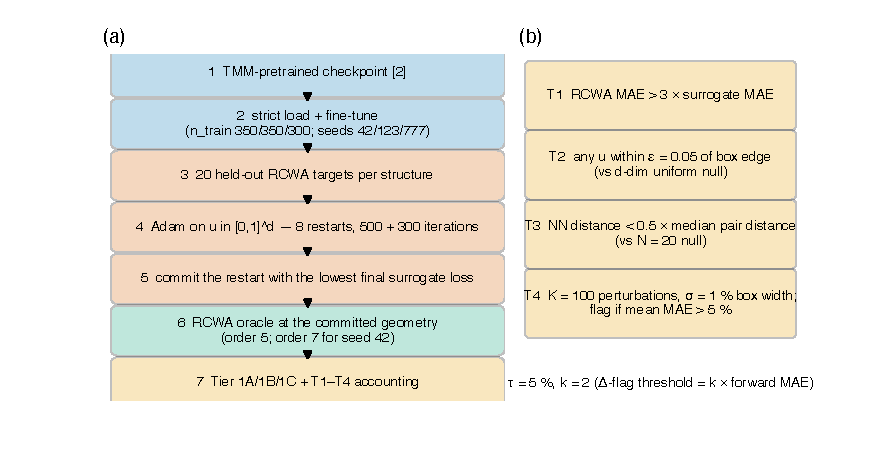
\includegraphics{figures/fig1_protocol_schematic.pdf}
\caption{Protocol overview. (a) Pipeline: the TMM-pretrained checkpoint regenerated with the recipe of {[}1{]} is strict-loaded and fine-tuned (n\_train 350 per structure; training seeds 42/123/777); 20 held-out RCWA targets per structure are inverted by Adam on the normalized geometry u with 8 restarts (500 + 300 iterations); the restart with the lowest final surrogate loss is committed; the committed geometry is evaluated once by the RCWA reference solver at its per-wavelength adaptive order; Tier 1A/1B/1C and the T1--T4 taxonomy are accounted. (b) Pre-specified thresholds: \ensuremath{\tau} = 5 \%, k = 2 (\ensuremath{\Delta}-flag threshold = k \ensuremath{\times} forward MAE), T1 factor 3, T2 \ensuremath{\varepsilon} = 0.05, T3 factor 0.5, T4 K = 100 perturbations with \ensuremath{\sigma} = 1 \% of the box width and a 5 \% mean-MAE flag.}
\label{fig:1}
\end{figure}

\textbf{Notation.} \emph{Structure} denotes one of the absorber families A, B and C of the
protocol, or the fourth family D of Section 3.12.
\emph{Surrogate MAE} is the mean absolute error of the surrogate\textquotesingle s predicted spectrum
against the target, and \emph{reference-solver MAE} the same quantity computed from the
RCWA solver at the same geometry, both over the 100 wavelength channels and in
percentage points. A design is \emph{surrogate-claimed} when its surrogate MAE is at or
below \ensuremath{\tau} and \emph{oracle-confirmed} when its reference-solver MAE is; a \textbf{pretender} is
surrogate-claimed but not oracle-confirmed. \ensuremath{\Delta} is the reference-solver MAE minus the
surrogate MAE at the committed geometry, and a design is \emph{\ensuremath{\Delta}-flagged} when \ensuremath{\Delta} exceeds
k times the surrogate\textquotesingle s forward test error. \ensuremath{\rho}(RCWA MAE, Surr MAE) is the Spearman
correlation of the two errors across the N targets of one run. The \emph{committed
geometry} \(g(u^*)\) is the geometry selected by the commitment rule. \emph{Preliminary r} and \emph{published
r} denote the two transferability conventions of Section 2.1.

\subsection{Fake-optimum taxonomy}\label{sec:2.4}

\begin{table}[htbp]
\centering
\setlength{\tabcolsep}{3pt}\footnotesize
\caption{Fake-optimum taxonomy (the four types and the diagnostic each one is measured by; nulls are defined in Section 2.5).}
\label{tab:3}
\begin{tabular}{@{}
  >{\RaggedRight\arraybackslash}p{(\linewidth - 6\tabcolsep) * \real{0.1823}}
  >{\RaggedRight\arraybackslash}p{(\linewidth - 6\tabcolsep) * \real{0.4088}}
  >{\RaggedRight\arraybackslash}p{(\linewidth - 6\tabcolsep) * \real{0.4088}}@{}}
\toprule\noalign{}
\begin{minipage}[b]{\linewidth}\raggedright
Type
\end{minipage} & \begin{minipage}[b]{\linewidth}\raggedright
Description
\end{minipage} & \begin{minipage}[b]{\linewidth}\raggedright
Diagnostic
\end{minipage} \\
\midrule\noalign{}
\textbf{T1} Oracle divergence & RCWA disagrees by more than a factor of three & \(\mathrm{MAE}(A_{\mathrm{RCWA}}, A^{*}) > 3\cdot\mathrm{MAE}(f_{NN}, A^{*})\) \\
\textbf{T2} Box-edge geometry & recovered geometry pressed to the design box & any normalized parameter within 0.05 of 0 or 1; vs \emph{d}-dim uniform null \\
\textbf{T3} Mode collapse & distinct targets funnel to one region & NN distance \textless{} 0.5 \ensuremath{\times} median pair distance; vs N = 20 uniform null \\
\textbf{T4} Surrogate-local smoothness & surrogate spectrum under K = 100 Gaussian perturbations, \ensuremath{\sigma} = 1 \% box width & mean perturbation MAE \textgreater{} 5 \% (measured, not merely defined) \\
\bottomrule\noalign{}
\end{tabular}
\end{table}

\subsection{Pre-specified thresholds and statistical plan}\label{sec:2.5}

Thresholds: \ensuremath{\tau} = 5 \% (engineering tolerance, the scale of the forward
MAE); k = 2 (a doubling buffer above the forward noise floor); T1 factor 3;
T2 \ensuremath{\varepsilon} = 0.05 (line-edge fabrication scale); T3 factor 0.5; T4 threshold 5 \%.

The pre-specified analysis plan:

\begin{enumerate}
\def\labelenumi{\arabic{enumi}.}
\tightlist
\item
  \textbf{Primary discrimination statistic: \ensuremath{\rho}(RCWA MAE, Surr MAE)} (Spearman,
  asymptotic p from SciPy \cite{al202043}, Bonett--Wright Fisher-z 95 \% CI \cite{bonett200044}; no exact or
  permutation inference is claimed). This is the clean "does surrogate
  confidence track the reference solver" quantity that H1c tests.
\item
  \ensuremath{\rho}(\ensuremath{\Delta}, Surr MAE) is reported \textbf{only as secondary with a coupling caveat}: \ensuremath{\Delta}
  contains \ensuremath{-}Surr by construction, so its negative bias is partly tautological.
  No "confidence inversion" language is used unless an effect survives in
  \ensuremath{\rho}(RCWA, Surr) itself --- which it does not.
\item
  Cross-structure count comparisons use \textbf{Fisher exact} tests \cite{fisher193545}; we state
  outright when differences at N = 20 are not significant.
\item
  T3 clustering can shrink the effective N; the cluster structure is reported
  alongside every count-based CI.
\item
  All seeds are fixed and logged: split 42, train-subset 42, targets 42,
  restarts \texttt{rng(1000\ +\ original-dataset\ index\ of\ the\ target)}, training 42,
  with the multi-seed extension at 123 and 777.
\end{enumerate}

\textbf{Test families and what is confirmatory.} The protocol names three confirmatory
comparisons --- the H1a--c orderings at seed 42 --- and does not specify a family-wise
correction. Everything else in Section 3 is exploratory and is reported with nominal
\emph{p}-values, with the following corrections applied as sensitivity analyses rather than as
decision rules: Holm over the nine per-run Spearman tests and over the nine pairwise
Fisher tests of Section 3.4; Holm over the two pooled control primaries of Sections 3.6
and 3.8, and over all ten control tests (six per-structure and two pooled Wilcoxon, two McNemar);
and for the 36 detector \ensuremath{\times} structure intervals of Table 10, an interval excluding 0.5 is
read as a selection from that screen, not as a pointwise confirmation. Where several seeds
share targets, the shared-target dependence is handled by one of three distinct
procedures, not interchangeably: a cluster bootstrap over targets (Table 10; the
percentile intervals of Section 3.4 and its 20\ensuremath{\rightarrow}50 extension); dividing each structure\textquotesingle s
counts and denominators by its design effect before the test (the pooled trend of Section
3.3; the effective-N Wilson interval of Section 3.4); or a plain nominal Wilson interval,
labelled as such, when neither adjustment is applied.

\subsection{Pilot-study defects corrected in the final protocol}\label{sec:2.6}

Two pilot studies preceded the protocol. A full AI-assisted internal audit of their code
found the eight defects listed below; every one was fixed before the protocol was
frozen, and no result reported in this paper depends on a pilot run. The
complete account, including the pilot headlines that were consequently dropped,
is given in Supplementary Section S5.

\begin{table}[htbp]
\centering
\setlength{\tabcolsep}{3pt}\footnotesize
\caption{Pilot-study defects and the corrections carried into the final protocol (the complete account is Supplementary Section S5).}
\label{tab:4}
\begin{tabular}{@{}
  >{\RaggedRight\arraybackslash}p{(\linewidth - 6\tabcolsep) * \real{0.0110}}
  >{\RaggedRight\arraybackslash}p{(\linewidth - 6\tabcolsep) * \real{0.7217}}
  >{\RaggedRight\arraybackslash}p{(\linewidth - 6\tabcolsep) * \real{0.2673}}@{}}
\toprule\noalign{}
\begin{minipage}[b]{\linewidth}\raggedright
\#
\end{minipage} & \begin{minipage}[b]{\linewidth}\raggedright
pilot defect
\end{minipage} & \begin{minipage}[b]{\linewidth}\raggedright
corrected protocol
\end{minipage} \\
\midrule\noalign{}
1 & B/C inverse run on 380--780 nm against 400--1800 nm data & per-structure native grids, pinned in artifacts \\
2 & Adam on raw nm --- optimizer frozen within \ensuremath{\pm}22 nm & normalized variables + multi-start (\S{}2.2) \\
3 & divergent RCWA rows leaked into train/test/targets --- an instance of the leakage failure catalogued across ML-based science {[}37{]} & Paper 1 filter (\S{}2.1) \\
4 & permuted pretrain input columns; phys stats recomputed on RCWA; C-bounds mismatch & faithful strict loading (\S{}2.1) \\
5 & T4 reported but never computed & implemented and measured (\S{}2.4) \\
6 & \ensuremath{\rho}(\ensuremath{\Delta}, Surr) "confidence inversion" headline (coupling artifact) & primary stat = \ensuremath{\rho}(RCWA, Surr) (\S{}2.5) \\
7 & A used 6 curated targets vs B\textquotesingle s 20 random --- the weak-baseline and reporting-bias pattern documented for ML applied to PDE problems {[}38{]} & identical N = 20 random targets for all structures \\
8 & single deterministic init; \texttt{manual\_seed} no-op & R = 8 multi-start, archived endpoints \\
\bottomrule\noalign{}
\end{tabular}
\end{table}

\subsection{Pre-specification record}\label{sec:2.7}

The protocol was frozen on \textbf{2026-06-10}, before the seed-42 runs of the as-submitted arm
(Section 3.10) and three months before the published-pipeline runs that form the main text,
and is reproduced verbatim in Supplementary Section S4. Its SHA-256 is
\texttt{\seqsplit{2e973ba41a82346f4724ff57aaf941dc79534a6e3d485c64dc6c61dd8c559e05}} and its git blob id is
\texttt{\seqsplit{e6d020fc3b69011fed4fc39834712da09621b0a9}}.

We state the timeline in full rather than claiming more than the record supports. The
seed-42 artifacts carry file timestamps of 2026-06-10 14:38--17:59 UTC, consistent with the
stated freeze. The protocol file itself was last modified on 2026-06-11 09:39 UTC, and two items in
the file as it now stands post-date the freeze. One is the restart-seeding sentence,
appended after an AI-assisted code review pointed out that the as-run seeding was
\texttt{rng(1000\ +\ original-dataset\ index\ of\ the\ target)} rather than the wording first used; it
records the as-run definition, which is a fixed, pre-data quantity, and all results use it.
The other is the parenthesis in \S{}5 item 5 naming training seeds 123 and 777 as a multi-seed
extension, which was appended after the seed-42 runs. The seed-123 and seed-777 artifacts
carry timestamps of 2026-06-10 23:46 to 2026-06-11 07:51 UTC, earlier than the file\textquotesingle s last
modification, so
the record cannot show that the extension was written down before those runs, and the
extension is classified as such in Table 5 rather than as pre-specified. What does \textbf{not}
exist is a contemporaneous public timestamp: the
protocol was not committed to version control or deposited anywhere before execution. The
surviving protocol is reproduced in Supplementary S4 as preserved, with its two post-freeze additions marked; the repository commit
that contains it post-dates the runs. Readers should weigh the pre-specification accordingly: the
freeze is documented internally and the analysis plan visibly constrains what we report, but
it is not third-party verifiable for this paper.

\textbf{Amendments made in September 2026, and what was known when.} The audit was designed
against the release of \cite{choi20261} that was current when the protocol was frozen. Three changes
followed, each recorded in the release archive with its date:

\begin{enumerate}
\def\labelenumi{\arabic{enumi}.}
\tightlist
\item
  \textbf{2026-09-06 --- the audited release changed.} On finding that the companion\textquotesingle s printed
  pipeline differs from the release the protocol was written against (regenerated pools,
  per-wavelength adaptive Fourier order, complex64, Johnson--Christy materials, and for
  Structure C a corrected normalization box and an 18-feature set), the whole protocol was
  re-run on the printed pipeline, which became the main text; the original arm is reported
  beside it in Section 3.10. Thresholds, hypotheses, target rule and metric hierarchy were
  not touched.
\item
  \textbf{2026-09-07 --- the control experiments were reduced to the canonical seed.} After the
  printed-pipeline rates were known (6 of 60 pretenders at seed 42), the from-scratch and
  feasibility controls were run at seed 42 only rather than at three seeds. The rationale
  recorded at the time was statistical --- that at this base rate three seeds would not give
  the binary comparison power. An AI-assisted review two days later judged that argument too
  strong: the seeds share one target set (Section 3.4), so they add correlated replicates
  rather than independent designs, but replicates do add some precision. The decision was
  kept on the ground that does hold, cost, and both the original and the revised reasoning
  are in the release archive. It was in any case a scope decision informed by the main-arm
  rate, and is disclosed as such.
\item
  \textbf{2026-09-08 --- the controls\textquotesingle{} primary outcome was changed, before any control output
  existed.} The protocol\textquotesingle s endpoint for the controls was the pretender count. At a base
  rate near 10 \% that comparison cannot resolve anything smaller than a rise to 23--35 \%
  (the range covers the possible joint distributions of the paired conditions), so the
  primary outcome became the \textbf{paired shift in \ensuremath{\Delta}}, tested by Wilcoxon signed-rank with a
  bootstrap interval on the median, with the pretender count retained as a secondary
  exact-McNemar comparison \textbf{and reported whatever it shows}, together with the minimum
  detectable effect. Those four elements --- pairing, the continuous primary, the binary
  secondary, and MDE reporting --- are what the dated amendment fixed. It did not specify how
  incomplete pairs are handled or a multiplicity correction across the two controls; the
  analysis script drops a pair whose solver call failed on either side, and the two control
  comparisons are reported at their nominal \emph{p} with Holm corrections over the two
  primaries and over all ten control tests as sensitivity analyses (Section 2.5), both
  choices made when the script was written and stated here rather than claimed as
  pre-specified. What was already
  known was the main arm\textquotesingle s rates; what did not yet exist was any control run --- the archived
  analysis file of that date records all six control conditions as absent. This is therefore an amendment informed by the main-arm
  results and fixed before the control results, not a pre-data plan, and not a choice made
  after seeing the comparison it governs.
\item
  \textbf{2026-09-16 to 09-19 --- the two controls were extended to seeds 123 and 777 after all.}
  Amendment 2 recorded the decision to run them at seed 42 only. After the seed-42 results
  and their analysis were written, an AI-assisted review recommended the extension as the
  more informative of two optional computations, on the ground amendment 2 already
  conceded --- correlated replicates still add precision. The runs used the identical
  pipeline and the identical analysis script, each seed analysed exactly as seed 42 was,
  plus a pooled block whose interval resamples targets with their three seeds together
  (Section 3.4). The extension is post hoc and is reported in Sections 3.6 and 3.8 as a
  replication of the seed-42 analysis, which is unchanged and remains the pre-specified
  comparison; the pooled signed-rank and McNemar \emph{p}-values are labelled nominal because
  the 179 pairs are 60 targets \ensuremath{\times} 3 correlated seeds.
\end{enumerate}

Table 5 states, for every analysis in Section 3, whether it was pre-specified in
that protocol or added afterwards.

\begin{table}[htbp]
\centering
\setlength{\tabcolsep}{3pt}\footnotesize
\caption{Pre-specification status of every analysis in Section 3 (pre-specified, extension, or post hoc exploratory, with the protocol section that fixes each pre-specified item).}
\label{tab:5}
\begin{tabular}{@{}
  >{\RaggedRight\arraybackslash}p{(\linewidth - 6\tabcolsep) * \real{0.3764}}
  >{\RaggedRight\arraybackslash}p{(\linewidth - 6\tabcolsep) * \real{0.5358}}
  >{\RaggedRight\arraybackslash}p{(\linewidth - 6\tabcolsep) * \real{0.0879}}@{}}
\toprule\noalign{}
\begin{minipage}[b]{\linewidth}\raggedright
analysis
\end{minipage} & \begin{minipage}[b]{\linewidth}\raggedright
status
\end{minipage} & \begin{minipage}[b]{\linewidth}\raggedright
protocol section
\end{minipage} \\
\midrule\noalign{}
H1a--c orderings, seed-42 Fisher and Spearman tests (\S{}3.3) & pre-specified & \S{}1, \S{}5 \\
Tier 1A--1C accounting and the T1--T4 taxonomy (\S{}3.2) & pre-specified & \S{}4 \\
Order-7 spot check of the three highest-\ensuremath{\Delta} geometries & pre-specified, superseded (\S{}3.5) & \S{}3.5 \\
Seeds 123 and 777 (\S{}3.4) & extension; timing relative to the runs not established & \S{}5 item 5 \\
Full order-7 revalidation of all seed-42 designs (legacy arm only) & post hoc exploratory & --- \\
Pooled counts with Wilson intervals, ICC and design effects (\S{}3.4) & post hoc exploratory & --- \\
Re-analysis under the published \emph{r} and the amplitude ordering (\S{}3.3) & post hoc exploratory & --- \\
Random-search and single-start commitment rules (\S{}3.6) & post hoc exploratory & --- \\
From-scratch (M0) and feasibility-constrained controls, paired \ensuremath{\Delta} primary (\S{}3.6, \S{}3.8) & amended 2026-09-08 after the main-arm rates, before any control output (\S{}2.7) & --- \\
T2-versus-pretender association, CMH (\S{}3.7) & post hoc exploratory & --- \\
Holm correction over the nine tests (\S{}3.3, \S{}3.4) & post hoc exploratory & --- \\
\ensuremath{\tau} sweep and the severity bands (\S{}3.4) & post hoc exploratory & --- \\
Power and minimum-detectable-effect analysis (\S{}3.3) & post hoc exploratory & --- \\
Surrogate-side detector benchmark (\S{}3.7) & post hoc exploratory & --- \\
Geometric feasibility cross-tabulation (\S{}3.8) & post hoc exploratory & --- \\
Lookup null and recoverability (\S{}3.9) & post hoc exploratory & --- \\
Structure D out-of-sample band (\S{}3.12) & recorded before the D runs; amended while 42/50 oracle results existed on disk, uninspected & --- \\
Fixed-order-5 cross-solver probe (\S{}3.11) & post hoc exploratory & --- \\
20\ensuremath{\rightarrow}50 target-set extension (\S{}3.4) & post hoc, unregistered; nested (the 20 protocol targets plus 30 more, same trained surrogates), not an independent sample & --- \\
\bottomrule\noalign{}
\end{tabular}
\end{table}

\begin{center}\rule{0.5\linewidth}{0.5pt}\end{center}

\section{Results}\label{sec:3}

Every table and figure is regenerated deterministically from the archived
per-run artifacts (SHA-256 manifest; Supplementary Sections S1, S2 and S6). Re-executing the
GPU training stages reproduces the results statistically rather than bitwise, since
CUDA training is not deterministic; the reference-solver stage, by contrast, is
bitwise reproducible: re-simulating 12 committed geometries (four per structure) with
the cache bypassed, against the vendored upstream commit, returns the archived absorptance
spectra exactly on both arms --- a maximum absolute deviation of 0 in every spectrum and of
0 percentage points in the resulting MAE (\texttt{repro\_\allowbreak{}check\_\allowbreak{}v8.\allowbreak{}json} in each arm\textquotesingle s archive; the
published-pipeline recheck at adaptive order took 6.2 GPU-hours). Every archived spectrum
also carries a fingerprint of the solver code and settings that produced it and is
re-validated against the live solver identity on every read.
The multi-seed runs are reported in Section 3.4 and the orders the
solver selected in Section 3.5.

\subsection{\texorpdfstring{Forward fine-tune fidelity against the published tables of \cite{choi20261}}{Forward fine-tune fidelity against the published tables of }}\label{sec:3.1}

The fine-tuned surrogates reproduce the forward performance that \cite{choi20261} prints,
confirming faithful loading: test absorptance MAE (A for Structures A/B; the mean of A\_TE and A\_TM for C) is
\textbf{B 1.72 \%, A 1.76 \%, C 2.11 \%} at seed 42, against the printed ten-seed values of
1.65 \ensuremath{\pm} 0.04, 1.79 \ensuremath{\pm} 0.04 and 2.05 \ensuremath{\pm} 0.09 \% (\textbar z\textbar{} \ensuremath{\leq} 1.7 on every structure;
\texttt{pub\_\allowbreak{}gate\_\allowbreak{}table123.\allowbreak{}json}). The pilot value of 5.17 \% arose from
unfaithful checkpoint loading, and the as-submitted release audited in Section 3.10
reaches only 3.2--4.8 \% because of its narrower bands, looser hygiene and the
Structure-C bound mismatch (Section 2.1). These forward MAEs set the per-structure
\ensuremath{\Delta}-flag thresholds of k = 2 \ensuremath{\times} MAE: \textbf{3.44 / 3.51 / 4.21 \% for B / A / C}.

\subsection{Per-structure reliability (seed 42)}\label{sec:3.2}

Every valid committed geometry was revalidated by the RCWA reference solver (torcwa
0.1.4.2 \cite{kim202346}, 64 \ensuremath{\times} 64 grid, per-wavelength adaptive Fourier order N \ensuremath{\in} \{9, 13, 17\} =
data-generating fidelity; Section 3.5). The
cross-structure picture, structures ordered by the published \emph{r} (B \textgreater{} A \textgreater{} C; Figure 2):

\begin{table}[htbp]
\centering
\setlength{\tabcolsep}{2pt}\tiny
\caption{Per-structure reliability at training seed 42 (Tier 1A--1C accounting, taxonomy counts and the primary discrimination statistic; columns ordered by the published \emph{r} of {[}1{]}, Table 5; preliminary \emph{r} from {[}1{]}, Supplementary S19).}
\label{tab:6}
\begin{tabular}{@{}llll@{}}
\toprule\noalign{}
Quantity & B (\emph{r} = +0.96; prelim. \ensuremath{-}0.07) & A (\emph{r} = +0.83; prelim. +0.72) & C (\emph{r} = +0.65; prelim. +0.34) \\
\midrule\noalign{}
n\_train & 350 & 350 & 350 \\
Forward test MAE & 1.72 \% & 1.76 \% & 2.11 \% \\
\textbf{Surrogate-claimed success} (\ensuremath{\tau} = 5 \%) & \textbf{20/20} & \textbf{20/20} & \textbf{20/20} \\
\textbf{Oracle-confirmed success} & 17/20 & 19/20 & 18/20 \\
\textbf{Pretenders} {[}Wilson 95 \% CI{]} & 3/20 {[}5.2, 36.0{]} & 1/20 {[}0.9, 23.6{]} & 2/20 {[}2.8, 30.1{]} \\
\ensuremath{\Delta}-flagged (k = 2) & 7/20 & 2/20 & 1/20 \\
\ensuremath{\Delta}-flag threshold & 3.44 \% & 3.51 \% & 4.21 \% \\
Max \ensuremath{\Delta} & 12.11 \% & 9.90 \% & 4.66 \% \\
Max amplification & 35.45\ensuremath{\times} & 43.62\ensuremath{\times} & 3.25\ensuremath{\times} \\
\ensuremath{\rho}(RCWA, Surr) --- \textbf{primary} & +0.12 (p = 0.62) & +0.34 (p = 0.14) & +0.75 (p \textless{} 0.001) \\
T1 / T2 / T3 / T4 (of 20) & 17 / 15 / 7 / 0 & 16 / 14 / 0 / 0 & 1 / 9 / 5 / 0 \\
Distinct modes (of 20) & 16 & 20 & 17 \\
\bottomrule\noalign{}
\end{tabular}
\end{table}

The two success rows carry the result: \textbf{every one of the 20 committed designs
passes the surrogate\textquotesingle s own success check on all three structures, and the reference
solver still rejects 1 to 3 of them per structure.} The threshold test is the part
that screens nothing out here: an optimizer that drives the surrogate\textquotesingle s own error to
0.06--4.6 \% leaves every design below \ensuremath{\tau}, so the verdict cannot separate the 54 the solver
confirms from the 6 it rejects. That is an observed property of this optimizer on these
targets, not a theorem --- a weaker surrogate or a harder target set could fail its own
check. That is a weaker statement
than the one the same protocol supports on the as-submitted release, where the solver
confirmed fewer than half (Section 3.10); here it agrees 85--95 \% of the time.

Two rows move in the opposite direction to the pretender counts and are worth reading
together with them. B carries \textbf{more} \ensuremath{\Delta}-flags than in the as-submitted release (7 of 20
against 6) even though it has a third as many pretenders, because the flag threshold is
k = 2 times each surrogate\textquotesingle s own forward MAE and that MAE has halved (3.44 \% here against
6.37 \%); Section 4.5 returns to this. And C\textquotesingle s primary discrimination statistic is
\ensuremath{\rho} = +0.75 (p \textless{} 0.001), so on that structure the surrogate\textquotesingle s continuous self-report does
order the reference-solver error even though its pass/fail verdict does not.

\begin{figure}[htbp]
\centering
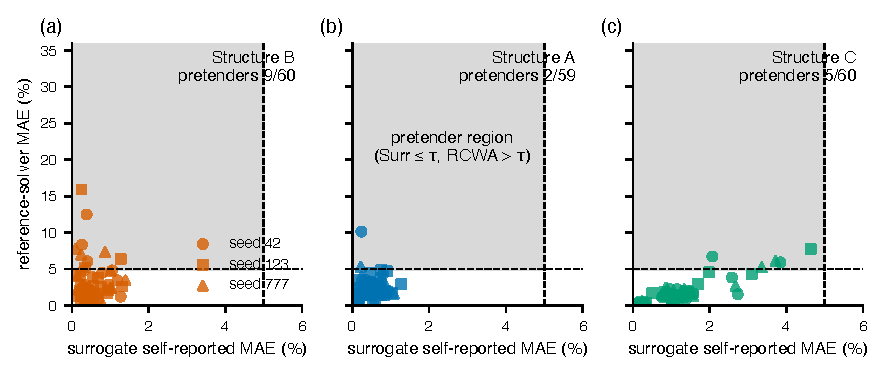
\includegraphics{figures/fig2_selfreport_vs_oracle.pdf}
\caption{Self-reported versus reference-solver error at every valid committed geometry, for all nine runs (three structures \ensuremath{\times} training seeds 42, 123 and 777; circles, squares and triangles respectively). Both axes are the mean absolute error (MAE) of the absorptance spectrum against the target over the 100 wavelength channels, in percentage points: on the abscissa as the surrogate reports it at its own committed geometry, on the ordinate as the RCWA reference solver measures it at the same geometry. Dashed lines mark the success threshold \ensuremath{\tau} = 5 \%; the shaded upper-left quadrant is the \emph{pretender} region, where the surrogate MAE is at or below \ensuremath{\tau} and the reference-solver MAE is above it. Every point lies left of the vertical line --- the surrogate certifies every design --- while 16 of the 179 lie above the horizontal one. The counts printed in each panel pool the three seeds.}
\label{fig:2}
\end{figure}

\subsection{Pre-specified hypothesis tests}\label{sec:3.3}

The three pre-specified orderings are evaluated under both \emph{r} conventions in
Table 7. \textbf{The pre-specified convention is the one H1a holds under; H1b and H1c hold under neither.} H1a --- oracle
success non-increasing as \emph{r} falls --- is monotone along the preliminary order
A, C, B at seed 42 (19 / 18 / 17) and over the pooled runs (57/59, 55/60, 51/60);
under the published \emph{r} it is not. The direction is the one the protocol predicted,
but at these counts a pairwise test cannot resolve it: the extreme pair A-vs-B gives
Fisher \emph{p} = 0.605.

\begin{table}[htbp]
\centering
\setlength{\tabcolsep}{3pt}\footnotesize
\caption{Pre-specified orderings under the two \emph{r} conventions (seed-42 counts, pooled in parentheses; "monotone" = non-increasing for H1a/H1c, non-decreasing for H1b, along the stated order).}
\label{tab:7}
\begin{tabular}{@{}
  >{\RaggedRight\arraybackslash}p{(\linewidth - 10\tabcolsep) * \real{0.1129}}
  >{\RaggedRight\arraybackslash}p{(\linewidth - 10\tabcolsep) * \real{0.2618}}
  >{\RaggedRight\arraybackslash}p{(\linewidth - 10\tabcolsep) * \real{0.2191}}
  >{\RaggedRight\arraybackslash}p{(\linewidth - 10\tabcolsep) * \real{0.2084}}
  >{\RaggedRight\arraybackslash}p{(\linewidth - 10\tabcolsep) * \real{0.1977}}@{}}
\toprule\noalign{}
\begin{minipage}[b]{\linewidth}\raggedright
Hypothesis
\end{minipage} & \begin{minipage}[b]{\linewidth}\raggedright
Quantity (seed 42; pooled)
\end{minipage} & \begin{minipage}[b]{\linewidth}\raggedright
Monotone under preliminary \emph{r} (A, C, B)?
\end{minipage} & \begin{minipage}[b]{\linewidth}\raggedright
Monotone under published \emph{r} (B, A, C)?
\end{minipage} & \begin{minipage}[b]{\linewidth}\raggedright
Smallest pairwise \emph{p} (nominal; Holm)
\end{minipage} \\
\midrule\noalign{}
H1a & oracle success 19 / 18 / 17 (57/59, 55/60, 51/60) & yes & no & 0.605 (1.000) \\
H1b & \ensuremath{\Delta}-flag rate 2 / 1 / 7 (7/59, 1/60, 16/60) & no & no & 0.044 (0.392) \\
H1c & \ensuremath{\rho}(RCWA, Surr) +0.34 / +0.75 / +0.12 & no & no & --- \\
--- & worst-case severity max \ensuremath{\Delta} 9.9 / 4.7 / 12.1 \% & no & no & --- \\
\bottomrule\noalign{}
\end{tabular}
\end{table}

A Cochran--Armitage trend test on the pooled pretender counts, scored by the \emph{r}
values themselves rather than by rank, is \textbf{nominally significant under the
pre-specified convention} (\emph{p} = 0.026) and remains so after the design effect of
the shared targets is applied (\emph{p} = 0.030, Section 3.4 --- an approximation that divides
each structure\textquotesingle s counts and denominators by its design effect before the trend test, not a
cluster permutation test); under the published \emph{r} it is
not (0.269 nominal, 0.221 corrected) and under the amplitude ordering it is flat
(0.981 nominal). Restricted to the canonical seed the same test gives \emph{p} = 0.292,
so the trend rests on the pooled runs, which Section 2.7 classifies as exploratory.

Two things bound how much this supports the diagnostic. The trend is carried by
\textbf{16 events across three structures}, and three points admit a monotone ordering by
chance with probability 1/6 under any single convention --- we tested three. And the
pairwise tests that would localise the effect do not reach significance. The honest
reading is that pretender incidence is \textbf{consistent with} the pre-specified ordering
in these three structures, not that the ordering is established.

\textbf{Ordering under the amplitude component.} The printed study reads \emph{r} together
with the operating-band TMM MAE and states that the forward benefit follows the
amplitude ordering (A 7.9 \% \textless{} B 8.9 \% \textless{} C 16.9 \%), not \emph{r}. Ranked that way the
pooled pretender counts are A 2/59, B 9/60, C 5/60 --- not monotone, and the trend test
is flat (\emph{p} = 0.981). On the published pipeline it is therefore the \emph{preliminary}
shape correlation, not the companion\textquotesingle s own preferred joint reading, that tracks
inverse reliability; on the as-submitted release neither did (Supplementary Section S8).

\subsection{Multi-seed robustness}\label{sec:3.4}

Pooling the three seeds (42 / 123 / 777) tests whether the seed-42 result is specific to that seed:

\begin{table}[htbp]
\centering
\setlength{\tabcolsep}{3pt}\footnotesize
\caption{Reliability pooled over the three training seeds (42 / 123 / 777; Wilson intervals on the pretender rates; \emph{r} column headings as in Table 6, from {[}1{]}).}
\label{tab:8}
\begin{tabular}{@{}
  >{\RaggedRight\arraybackslash}p{(\linewidth - 10\tabcolsep) * \real{0.2053}}
  >{\RaggedRight\arraybackslash}p{(\linewidth - 10\tabcolsep) * \real{0.1987}}
  >{\RaggedRight\arraybackslash}p{(\linewidth - 10\tabcolsep) * \real{0.1987}}
  >{\RaggedRight\arraybackslash}p{(\linewidth - 10\tabcolsep) * \real{0.1987}}
  >{\RaggedRight\arraybackslash}p{(\linewidth - 10\tabcolsep) * \real{0.1987}}@{}}
\toprule\noalign{}
\begin{minipage}[b]{\linewidth}\raggedright
Quantity
\end{minipage} & \begin{minipage}[b]{\linewidth}\raggedright
B (\emph{r} = +0.96; prelim. \ensuremath{-}0.07)
\end{minipage} & \begin{minipage}[b]{\linewidth}\raggedright
A (\emph{r} = +0.83; prelim. +0.72)
\end{minipage} & \begin{minipage}[b]{\linewidth}\raggedright
C (\emph{r} = +0.65; prelim. +0.34)
\end{minipage} & \begin{minipage}[b]{\linewidth}\raggedright
Pooled
\end{minipage} \\
\midrule\noalign{}
Surrogate-claimed success & 60/60 & 59/59\dag{} & 60/60 & \textbf{179/179} \\
Oracle-confirmed success & 51/60 & 57/59 & 55/60 & 163/179 \\
\textbf{Pretenders} {[}Wilson 95 \% CI{]} & 9/60 {[}8.1, 26.1{]} & 2/59 {[}0.9, 11.5{]} & 5/60 {[}3.6, 18.1{]} & \textbf{16/179 (8.9 \%) {[}5.6, 14.0{]}} \\
\ensuremath{\Delta}-flagged (k = 2) & 16/60 & 7/59 & 1/60 & 24/179 \\
\ensuremath{\rho}(RCWA, Surr) per seed & +0.117 / +0.146 / \ensuremath{-}0.119 & +0.340 / +0.454 / +0.186 & +0.750 / +0.829 / +0.719 & range \ensuremath{-}0.119 \ldots{} +0.829 \\
\bottomrule\noalign{}
\end{tabular}
\end{table}

\dag{}One A geometry at seed 777 was degenerate and its solver call failed, so A\textquotesingle s
denominator is 59 (179 valid of 180). In the as-submitted release the failing geometry
was in C instead.

The pooled rate is \textbf{16/179 = 8.9 \%} (per-run counts and intervals in Supplementary
Table S1; Figure 3a). Its
nominal Wilson 95 \% CI is {[}5.6, 14.0{]} \%, but the 20 targets of a
structure are bit-identical across its three seeds, so the runs are correlated:
the intraclass correlation is 0.79 on C, 0.10 on B and \ensuremath{-}0.02 on A, for design
effects of 2.58 / 1.21 / 0.96 and effective sizes of 23 / 50 / 61. The pooled
design effect of 1.33 leaves the information of \textasciitilde134 designs, widening the
interval to {[}5.2, 15.0{]} \% (cluster bootstrap: {[}4.0, 14.5{]} \%), so we treat the
per-seed counts (B 3/3/3, A 1/0/1, C 2/1/2 of 20; A at seed 777 of 19) as primary. The rate is
strongly \ensuremath{\tau}-dependent (Figure 4), and this is the most consequential number in the
section: tightening the tolerance to \ensuremath{\tau} = 2.5 \% turns \textbf{53 of the 171 designs the
surrogate still certifies into pretenders (31 \%)}, while loosening it to 7.5 \% leaves
6/179 and to 10 \% leaves 3/179. Of the \ensuremath{\tau} = 5 \% pretenders 10 are mild (5--7.5 \%),
3 moderate and 3 severe (\ensuremath{\geq} 10 \%). The pretender rate is therefore a property of the
tolerance the design task demands, not a fixed property of the surrogate.

As a post-hoc target-set extension --- not a redefinition of the primary 20-target
protocol above, and not an independent replication of it --- the same trained surrogates
were run on 50 targets per structure, the original 20 plus 30 more drawn by the identical
mechanism; the 20-target counts of Table 8 are therefore a subset of the 50-target counts
below, not a separate sample. Pooling the three seeds over 50 \ensuremath{\times} 3 = 150 target-seed
slots per structure (147 valid on A, where three slots hit the same class of
degenerate-geometry solver failure as in the 20-target run; 150 on B and C) gives
a pooled pretender rate of \textbf{42/447 = 9.4 \%} (nominal Wilson 95 \% CI {[}7.0, 12.5{]};
design-effect-adjusted {[}6.8, 12.9{]} at n\_eff = 348; cluster bootstrap over targets,
20,000 reps, {[}6.3, 12.8{]}) --- overlapping the 20-target estimate of 8.9 \% {[}5.2, 15.0{]}.
The per-structure ordering is unchanged (A 5/147 = 3.4 \%, C 14/150 = 9.3 \%,
B 23/150 = 15.3 \%), the per-structure design effects are similar in direction and
magnitude (A 0.94, B 1.17, C 2.38 at 50 targets vs. 0.96 / 1.21 / 2.58 at 20 targets),
and the \ensuremath{\tau}-sensitivity pattern is repeated on the larger set: tightening \ensuremath{\tau} to 2.5 \% turns
155 of the 426 still-certified designs into pretenders (36.4 \%, cluster bootstrap
{[}30.9, 42.2{]}) at 50 targets, the same qualitative collapse as the 31 \% figure at 20
targets. Because the two counts overlap and share the same trained surrogates, this is
descriptive consistency with the original estimate, not an independent confirmation of
it; we therefore continue to treat the 20-target result as the pre-specified primary
estimate and report the 50-target numbers as an unregistered sensitivity check that
does not, on its own, change the sign or approximate magnitude of that estimate.

Whether the continuous self-report carries rank information depends on the structure.
\ensuremath{\rho}(RCWA, Surr) spans \ensuremath{-}0.119 to +0.829 over the nine runs; four are nominally significant
--- all three C runs (+0.750, +0.829, +0.719; p \ensuremath{\leq} 0.0004) and A \texttt{s123} (+0.454,
p = 0.044) --- and \textbf{the three C runs survive the nine-test Holm correction}
(adjusted p = 0.0011, 0.00006, 0.0025) while A \texttt{s123} does not (0.27).
(Exploratory) seed-pooled block permutation gives \ensuremath{\rho} = \ensuremath{-}0.01 (B, p = 0.94),
+0.33 (A, p = 0.080), +0.76 (C, p = 0.0002). As a detector of pretenders the
surrogate\textquotesingle s own claimed MAE has a pooled AUROC (Table 10\textquotesingle s seed-stratified estimator)
of 0.40 on B, 0.27 on A and \textbf{0.98 on C}: on B and A the pretenders are, if anything, the designs the surrogate
is \emph{most} confident about, whereas on C the surrogate\textquotesingle s error ranking is nearly
perfect even though its pass/fail verdict admits every design (Section 3.7).

\begin{figure}[htbp]
\centering
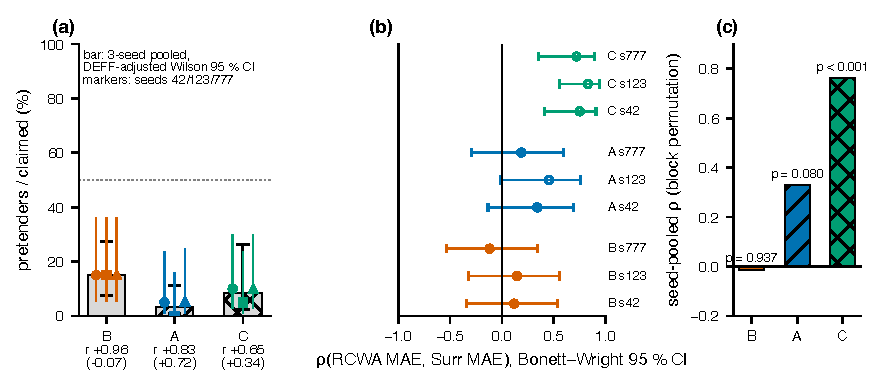
\includegraphics{figures/fig3_r_vs_reliability.pdf}
\caption{Transferability versus inverse reliability. A design is \emph{surrogate-claimed} when the surrogate\textquotesingle s own mean absolute error (MAE) against the target is at or below \ensuremath{\tau} = 5 \%, and a \emph{pretender} when it is claimed but the RCWA reference solver puts the MAE above \ensuremath{\tau}. (a) Pretenders per surrogate-claimed design for each run (markers: training seeds 42, 123 and 777, with Wilson 95 \% intervals) and the three-seed pooled rate (bar) with a design-effect-adjusted Wilson interval; dotted line: coin flip. Tick labels give the published \emph{r} and, in parentheses, the preliminary \emph{r} in force when the protocol was frozen --- both are measurements of {[}1{]} (Table 5; Supplementary S19); the inverse-reliability quantities are from the present study. (b) \ensuremath{\rho}(reference-solver MAE, surrogate MAE) per run with Bonett--Wright 95 \% intervals; open markers are the four nominally significant runs. (c) Seed-pooled within-structure \ensuremath{\rho} with block-permutation p (targets permuted jointly across seeds; exploratory).}
\label{fig:3}
\end{figure}

\begin{figure}[htbp]
\centering
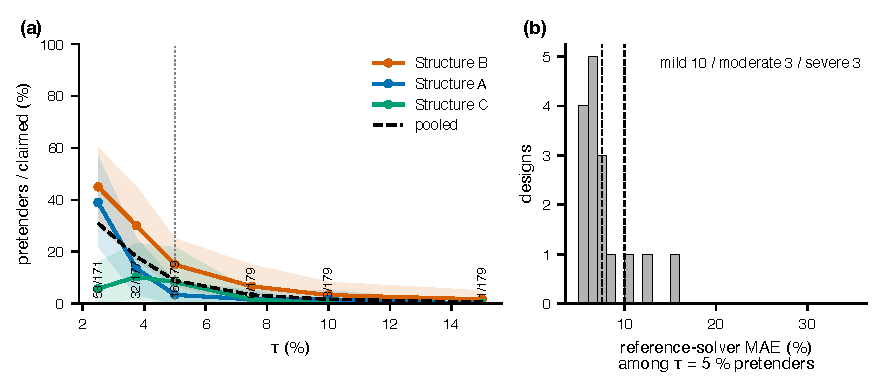
\includegraphics{figures/fig4_tau_sensitivity.pdf}
\caption{Sensitivity to the success threshold (exploratory; all nine runs, training seeds 42, 123 and 777 pooled). (a) Pretenders per surrogate-claimed design as \ensuremath{\tau} is varied, per structure and pooled, where at each \ensuremath{\tau} a design counts as claimed if the surrogate\textquotesingle s mean absolute error (MAE) is at or below \ensuremath{\tau} and as a pretender if the reference-solver MAE additionally exceeds \ensuremath{\tau}; bands are a cluster bootstrap over the 20 targets of each structure and the labels give the pooled pretender/claimed counts, whose denominator falls from 179 to 171 as \ensuremath{\tau} tightens to 2.5 \%. (b) Distribution of the reference-solver MAE among the \ensuremath{\tau} = 5 \% pretenders, with the post-hoc mild / moderate / severe band edges at 7.5 \% and 10 \%.}
\label{fig:4}
\end{figure}

\subsection{Per-wavelength adaptive order of the reference solver}\label{sec:3.5}

The published pipeline chooses the Fourier truncation per wavelength from
N \ensuremath{\in} \{9, 13, 17\} by the companion\textquotesingle s feature-size rule rather than fixing it, so the
fidelity of the audit varies with the geometry it is asked to resolve rather than with a
number set in advance. The audit therefore evaluates every committed geometry at exactly
the fidelity its training labels were generated at --- the same vendored routine decides
the order --- which is what "reference fidelity" means throughout. Across the
18 000 wavelength solves behind the nine runs of Sections 3.2 and 3.4 the solver used N = 17 on \textbf{59 \%} of
them, N = 13 on 7 \% and N = 9 on 35 \% (\texttt{adaptive\_\allowbreak{}orders\_\allowbreak{}v10.\allowbreak{}json}), and the
split is strongly per structure: Structure A runs at N = 17 on 98 \% of its wavelengths
and C on 75 \%, while B is at N = 9 on 83 \%. That is also where the cost goes: a
committed A geometry takes about 58 min to validate against 3 min for B. That cost is
the one the companion\textquotesingle s convergence study reports per wavelength at N = 17 (\ensuremath{\approx} 28 s; \cite{choi20261},
Supplementary S16) multiplied by the 100-wavelength grid; nearly every A geometry, in the
dataset as in the committed set, has a metal feature or gap below the rule\textquotesingle s 150-nm
threshold and is therefore solved at N = 17 throughout.

This replaces the fixed-order-7 revalidation the protocol specified. That check existed to
bound the error of a solver pinned at order 5 --- the companion\textquotesingle s convergence study (\cite{choi20261},
Supplementary S16) reports N = 5 absorptance discrepancies of \ensuremath{\approx} 2 pp on A, \ensuremath{\approx} 3 pp on B and
\ensuremath{\approx} 5 pp on C (TE), reaching \ensuremath{\approx} 6 pp and \ensuremath{\approx} 15 pp respectively at long wavelengths --- and
re-running at 7 would now
\emph{lower} the fidelity of a solver already at 9 to 17. The order-7 results for the
as-submitted arm, where they do apply, are in Supplementary Section S3. What the adaptive
order does \textbf{not} give is a convergence proof: the solver reports cases it cannot converge
at its cap of 17, so these are reference-fidelity statements (Section 4.7, W8). Section 3.11 re-solves the
same committed geometries, on the same 64 \ensuremath{\times} 64 raster, at a fixed order 5 and measures what
the order alone contributes.

\begin{figure}[htbp]
\centering
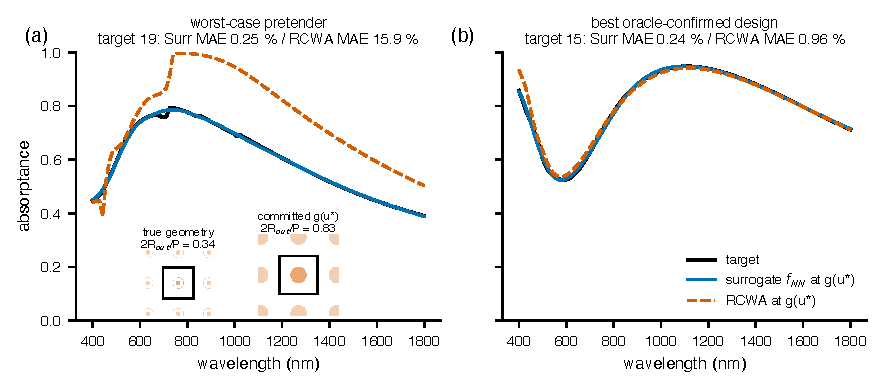
\includegraphics{figures/fig6_worst_pretender_spectrum.pdf}
\caption{Structure B, seed 123, absorptance channel. (a) Worst-case pretender (target 19 of 20): target spectrum, surrogate prediction at the committed geometry g(u*) with self-reported MAE 0.25 \%, and the reference solver at the same geometry with MAE 15.9 \%. The committed ring has \textbf{R\_in = 253 nm against R\_out = 208 nm} --- an inner radius larger than the outer one, which the generator\textquotesingle s sampling rule (R\_in \ensuremath{\leq} R\_out \ensuremath{-} 10 nm) can never produce, so the optimizer has placed its optimum outside the generator-feasible region entirely rather than merely at its edge. Its true counterpart is an ordinary ring (R\_out = 114 nm, R\_in = 104 nm, 2R\_out/P = 0.34). (b) Best oracle-confirmed design of the same run (target 15: self-reported MAE 0.24 \%, reference-solver MAE 0.96 \%), whose self-report is indistinguishable from the pretender\textquotesingle s. Target spectra are held-out samples of the published Structure-B dataset of {[}1{]}; the surrogate and reference spectra at the committed geometries were computed for this study.}
\label{fig:5}
\end{figure}

\subsection{Commitment rules and the from-scratch control (exploratory)}\label{sec:3.6}

Is the pretender phenomenon a gradient-exploitation artifact, or a generic
consequence of committing to the surrogate\textquotesingle s best point? At seed 42 we compare
three commitment rules under a matched evaluation budget:

\begin{table}[htbp]
\centering
\setlength{\tabcolsep}{3pt}\scriptsize
\caption{Pretenders under three commitment rules at a matched evaluation budget (seed 42; \emph{r} headings from {[}1{]}; pretenders / surrogate-claimed designs, the same quantity Figure 6 plots, with the oracle-confirmed count in parentheses. Supplementary Sections S2 and S8.2 give both quantities for both arms.)}
\label{tab:9}
\begin{tabular}{@{}llll@{}}
\toprule\noalign{}
Commitment rule & B (\emph{r} = +0.96; prelim. \ensuremath{-}0.07) & A (\emph{r} = +0.83; prelim. +0.72) & C (\emph{r} = +0.65; prelim. +0.34) \\
\midrule\noalign{}
Budget-matched random search & 6/20 (14 confirmed) & 4/20 (16 confirmed) & 1/16 (15 confirmed) \\
Gradient, best of 8 restarts & 3/20 (17 confirmed) & 1/20 (19 confirmed) & 2/20 (18 confirmed) \\
Gradient, single start & 4/19 (15 confirmed) & 4/19 (15 confirmed) & 4/15 (11 confirmed) \\
\bottomrule\noalign{}
\end{tabular}
\end{table}

(pretenders over surrogate-claimed designs, so the denominator is the number of
designs each rule certified; Figure 6; full table with both denominators, mean oracle MAEs, and
Fisher tests in Supplementary Section S2). \textbf{Every rule manufactures pretenders}, so
the gradient loop is \textbf{not necessary} for the phenomenon, in the same sense Section 3.8
uses for transferred weights and geometric infeasibility: removing it does not remove
pretenders, but this comparison does not isolate the gradient loop\textquotesingle s own contribution,
if any. Budget-matched random search
produces more of them than best-of-eight gradient descent on B and A (6/20 against
3/20; 4/20 against 1/20) and fewer on C (1/16 against 2/20), and none of the three
comparisons is significant at these counts (Fisher p = 0.45 / 0.34 / 1.00). Single-start
gradient is at or above best-of-eight everywhere (4/19, 4/19, 4/15): this argues against
restart selection pressure being what \emph{creates} pretenders, but --- as with the other two
controls --- it does not by itself identify what does. What the pub-arm
counts no longer support is the stronger claim that a weaker optimizer is \emph{reliably}
worse: on C random search both certified fewer designs (16 of 20) and had the single
lowest pretender count. Selecting the argmin of an imperfect learned objective is
enough, on its own, to produce pretenders under every one of the three rules tested ---
consistent with the surrogate-gaming pathology of offline
model-based optimization \cite{kumar202013,trabucco202114,trabucco202215,fannjiang202016}, here on a physical inverse-design testbed --- but,
as in Section 3.8, this does not establish it as the sole or necessary cause, and this
study cannot rank the commitment rules against each other.

\textbf{From-scratch control.} The same architecture trained from random initialization rather
than from the TMM-pretrained checkpoint (M0, learning rate 10\textsuperscript{\ensuremath{-}}\textsuperscript{3} from the upstream
from-scratch recipe) reaches a forward test MAE of 1.89, 2.59 and 1.96 \% on B, A and C
against the transfer-learned 1.72, 1.76 and 2.11 \%, so it is a surrogate of comparable
accuracy, and it draws the same targets --- the split is fixed before the training subset,
so M0 and the transfer-learned run are paired design by design. Over the 60 paired designs
the signed-rank test does not reject no-shift (Wilcoxon \emph{p} = 0.176); its estimand, the
Hodges--Lehmann shift in \ensuremath{\Delta}, is \textbf{+0.22 pp} {[}\ensuremath{-}0.09, +0.58{]}, the median shift is +0.14 pp
{[}\ensuremath{-}0.07, +0.44{]} (bootstrap), the mean +0.06 pp, and 27 designs move down against 33 up.
The pretender counts go \textbf{6 \ensuremath{\rightarrow} 4} (discordant 4/2, exact McNemar \emph{p} = 0.688). Per structure
the median shift is B \ensuremath{-}0.36 pp (\emph{p} = 0.216), A +0.75 pp (\emph{p} = 0.0017; Hodges--Lehmann
+0.92 pp {[}+0.32, +1.67{]}), C \ensuremath{-}0.03 pp (\emph{p} = 0.622): the from-scratch A surrogate, whose
forward MAE is 47 \% higher than the transfer-learned one, is measurably worse at the
committed geometries, while B and C are not.

\emph{Replication at seeds 123 and 777 (post hoc, Section 2.7 amendment 4).} The same control
at the other two training seeds gives Hodges--Lehmann shifts of +0.17 pp {[}\ensuremath{-}0.15, +0.50{]}
(Wilcoxon \emph{p} = 0.283; pretenders 4 \ensuremath{\rightarrow} 6) and +0.42 pp {[}+0.15, +0.73{]} (\emph{p} = 0.0025;
6 \ensuremath{\rightarrow} 7), and the from-scratch A surrogate is again the less accurate one at every seed
(forward MAE 2.62 and 2.57 \% against 1.78 and 1.68 \%, with B and C within 0.2 pp of their
transfer-learned counterparts). Over the 179 pairs of all three seeds the median shift is
\textbf{+0.20 pp {[}+0.03, +0.38{]}} with the interval clustered by target (a target\textquotesingle s three seeds
resampled together; Hodges--Lehmann +0.27 pp, nominal), the pretender counts are \textbf{16 \ensuremath{\rightarrow} 17}
(discordant 11/12), and the per-structure pattern replicates: A +0.82 pp {[}+0.55, +1.32{]}
with pretenders 2 \ensuremath{\rightarrow} 7, B +0.02 pp {[}\ensuremath{-}0.24, +0.61{]} with 9 \ensuremath{\rightarrow} 5, C +0.01 pp {[}\ensuremath{-}0.10, +0.14{]}
with 5 \ensuremath{\rightarrow} 5 (\texttt{control\_\allowbreak{}analysis\_\allowbreak{}v10\_\allowbreak{}3seed.\allowbreak{}json}).

Transferred weights are therefore not necessary for pretenders: a surrogate trained
without them produces them at a rate this design cannot distinguish from the
transfer-learned one (6 against 4 at the pre-specified seed, 16 against 17 over three),
and the pooled shift in \ensuremath{\Delta} is small and positive --- about a fifth of a percentage point
over three seeds, carried entirely by the structure on which the from-scratch surrogate
is less accurate. The interval is what carries that statement --- the binary comparison on
its own could not distinguish 6 from 4, and at this base rate it would only reach 80 \%
power against a control rate of 23--35 \% depending on how the two conditions co-occur, so
we report the bound rather than a bare null. Section 2.7 records that this analysis was
fixed after the main-arm rates were known and before any control output existed.

\begin{figure}[htbp]
\centering
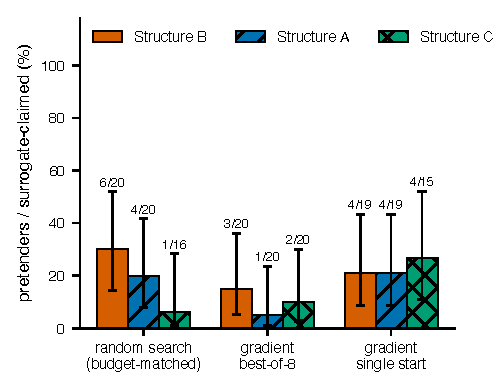
\includegraphics{figures/fig7_mechanism.pdf}
\caption{Pretenders per surrogate-claimed design at training seed 42 under three rules for choosing which geometry to commit: random search over 6400 uniform draws from the design box --- \emph{budget-matched}, i.e. given the same number of surrogate evaluations as the gradient loop\textquotesingle s 8 restarts \ensuremath{\times} 800 iterations --- gradient descent with the best of 8 restarts, and gradient descent from the single mid-box start. Wilson 95 \% intervals; k/n labels give pretenders over surrogate-claimed designs, so the denominators differ between rules (C random search: 1/16). Committing to the surrogate argmin suffices to produce pretenders under every rule, without isolating which of the three commitment mechanisms, if any, is the larger contributor; no pairwise difference between the rules is significant at these counts.}
\label{fig:6}
\end{figure}

\subsection{Surrogate-side diagnostics}\label{sec:3.7}

No cheap, oracle-free diagnostic flags the pretenders on every structure:

\begin{itemize}
\tightlist
\item
  \textbf{T4 surrogate-local smoothness} (measured, K = 100): \textbf{0/179 flags}; the mean
  perturbation MAE averages 0.79--1.12 \% per run and never exceeds 2.97 \%. The
  pre-specified finite-scale perturbation threshold is therefore not exceeded at any
  committed geometry; this does not rule out roughness at other scales or directions.
\item
  \textbf{Multi-start dispersion} (Tier 1C): the spread of the eight restarts\textquotesingle{} final losses
  is small (standard deviation 5 \ensuremath{\times} 10\textsuperscript{\ensuremath{-}}\textsuperscript{4} to 2.4 \ensuremath{\times} 10\textsuperscript{\ensuremath{-}}\textsuperscript{3} in MSE units per run, against
  committed losses of order 10\textsuperscript{\ensuremath{-}}\textsuperscript{4}--10\textsuperscript{\ensuremath{-}}\textsuperscript{3}) while the \emph{endpoint geometric} spread is large
  (1.36--1.88 in u-space) --- distinct basins with comparably low claimed loss, itself
  uninformative about which basin is real. The loss-tail RSD of the committed run
  (0.002--0.012) indicates stable terminal loss traces; it does not establish that the
  geometry or gradient had stopped changing.
\item
  \textbf{T2 box-edge} flags remain abundant (9--18/20 per run) but the association with
  pretender status that the as-submitted release showed \textbf{does not reproduce here}:
  the Cochran--Mantel--Haenszel estimate is OR 2.18 with p = 0.246, and no per-run
  Fisher test is significant. As a detector it is worse than before in the way that
  matters: sensitivity 0.75 and specificity 0.37 give a PPV of 0.10 against a base
  rate of 0.089, so flagging every box-edge design would reject nearly two thirds of
  the good designs to catch three quarters of a much smaller bad set. The
  flag also partly proxies geometric infeasibility (Section 3.8). At seed 42, T3 mode
  collapse appears on B and C (7 and 5 of 20) but not A; A does exhibit T3 at seed 123,
  so this is a seed-42 statement.
\end{itemize}

None of them is usable as a detector on its own across structures. Pooling the three
seeds within each structure gives the following areas under the ROC curve for separating
pretenders from oracle-confirmed designs (0.5 = chance):

\begin{table}[htbp]
\centering
\setlength{\tabcolsep}{3pt}\scriptsize
\caption{Discrimination of the oracle-free diagnostics (area under the ROC curve for separating pretenders from oracle-confirmed designs; the pooled value is the per-run AUROC averaged over the three seeds with weights n\_pretender \ensuremath{\times} n\_confirmed, so that seeds are never compared across runs, and the interval is a 2000-draw cluster bootstrap over targets in which a target\textquotesingle s three seeds are resampled together; draws without a pretender are discarded, so the intervals are conditional on that: on A, with two pretenders, 1716--1779 of the 2000 draws were usable and its intervals are exploratory (C 1744--1780, B 1998--2000); 36 cells are screened, so an interval excluding 0.5 is a selection, not a pointwise confirmation; 0.5 = chance; \texttt{detector\_\allowbreak{}bench\_\allowbreak{}v8.\allowbreak{}json}).}
\label{tab:10}
\begin{tabular}{@{}llll@{}}
\toprule\noalign{}
oracle-free quantity & B AUROC {[}95 \% CI{]} & A AUROC {[}95 \% CI{]} & C AUROC {[}95 \% CI{]} \\
\midrule\noalign{}
3-seed ensemble disagreement & 0.80 {[}0.63, 0.94{]} & 0.73 {[}0.42, 1.00{]} & 0.95 {[}0.88, 1.00{]} \\
held-out ensemble MAE & 0.75 {[}0.53, 0.91{]} & 0.51 {[}0.26, 0.79{]} & 0.98 {[}0.89, 1.00{]} \\
ensemble-mean MAE & 0.73 {[}0.52, 0.89{]} & 0.38 {[}0.16, 0.60{]} & 0.98 {[}0.84, 1.00{]} \\
distance to the fine-tune set & 0.80 {[}0.63, 0.94{]} & 0.73 {[}0.50, 0.94{]} & 0.42 {[}0.16, 0.61{]} \\
distance to the dataset pool & 0.79 {[}0.62, 0.92{]} & 0.73 {[}0.50, 1.00{]} & 0.49 {[}0.30, 0.78{]} \\
TMM--surrogate disagreement & 0.42 {[}0.23, 0.63{]} & 0.62 {[}0.39, 0.84{]} & 0.23 {[}0.00, 0.46{]} \\
TMM--target disagreement & 0.43 {[}0.24, 0.63{]} & 0.62 {[}0.38, 0.84{]} & 0.22 {[}0.00, 0.44{]} \\
T4 local-smoothness value & 0.48 {[}0.20, 0.77{]} & 0.92 {[}0.79, 1.00{]} & 0.66 {[}0.44, 0.87{]} \\
T2 box-edge flag & 0.62 {[}0.49, 0.75{]} & 0.66 {[}0.57, 0.77{]} & 0.46 {[}0.35, 0.60{]} \\
multi-start final-loss spread (std over the 8 restarts) & 0.50 {[}0.29, 0.68{]} & 0.27 {[}0.00, 0.63{]} & 0.74 {[}0.54, 0.92{]} \\
the surrogate\textquotesingle s own claimed MAE & 0.40 {[}0.19, 0.67{]} & 0.27 {[}0.09, 0.49{]} & 0.98 {[}0.89, 1.00{]} \\
generator-infeasibility flag & 0.76 {[}0.68, 0.86{]} & 0.74 {[}0.63, 0.87{]} & 0.37 {[}0.28, 0.46{]} \\
\bottomrule\noalign{}
\end{tabular}
\end{table}

The picture is structure-specific rather than uniformly null. On \textbf{C}, every
ensemble-based quantity and the surrogate\textquotesingle s own claimed MAE reach 0.95--0.98 with
intervals excluding 0.5: the C surrogate knows, in rank order, which of its designs are
wrong: in every C run the pretenders sit among the four designs with the largest claimed
MAE, so re-simulating the worst-ranked fifth of each run would catch all of them. On \textbf{B}, the distance to the nearest dataset point (0.79--0.80), the
ensemble quantities (0.73--0.80) and the infeasibility flag (0.76) exclude 0.5 but none
exceeds 0.81, while the claimed MAE is \emph{below} chance (0.40). On \textbf{A}, with only two
pretenders in 59 designs, only the T4 perturbation value (0.92), the two binary flags
(0.66, 0.74) and the claimed MAE --- again below chance (0.27) --- have intervals excluding 0.5.
No single quantity separates the two classes on all three structures, and the one that
works best on C --- the surrogate\textquotesingle s own error --- is the one that ranks pretenders as the
\emph{most} trustworthy designs on A and B.

Reference-solver evaluation determines the audit\textquotesingle s labels by definition, and no tested
diagnostic perfectly separated pretenders from confirmed designs on every structure: one oracle
call per design (103--4595 s at the adaptive order, median 1655 s), applying the decision
rule of Section 2.3 (surrogate-claimed, Surr MAE \ensuremath{\leq} \ensuremath{\tau}, \textbf{and} reference-solver MAE \textgreater{} \ensuremath{\tau}).
\ensuremath{\Delta}, the gap between the two MAEs, is not that decision rule --- it is reported separately,
as severity (Section 2.3, Tier 1B).

\subsection{Geometric feasibility of the committed designs (post hoc)}\label{sec:3.8}

The datasets are generated under structure-specific fabrication constraints (\cite{choi20261},
Supplementary S17) --- patch widths
at most 0.9 P for A and C, and for B an outer ring radius at most 0.45 P with each inner
radius at least 10 nm smaller than the one enclosing it --- but the optimizer searches the raw
sampling box, which does not enforce them. It leaves it: over the three seeds, 33/60
committed B geometries, 33/59 A and 13/60 C violate a constraint that every training
sample satisfies. This is not a surprise --- a uniform draw from the box is infeasible with
probability 0.77 on B, 0.56 on A and 0.52 on C --- but on B it matters, because there every
pretender is infeasible: 9 of the 33 infeasible B designs are pretenders against 0 of the
27 feasible ones (Fisher p = 0.0029; run-stratified CMH p = 0.0036). On A the two
pretenders are also infeasible but the count is too small to test (2/33 against 0/26,
p = 0.50), and on C the association runs the other way (0/13 against 5/47, p = 0.58): the
C pretenders are generator-feasible. A feasibility check is free, requires no solver call, and
on B is the one oracle-free signal that both carries information (Table 10, AUROC 0.76)
and needs no ensemble, which is why Section 3.7 is stated per structure rather than as a
blanket negative. Figure S1 shows where in the design box the committed geometries sit.

\textbf{Constrained rerun.} Repeating the seed-42 inverse design over a nested
parametrization whose image is exactly the generator\textquotesingle s feasible region --- every candidate
generator-feasible by construction, so the optimizer cannot leave it --- changes the outcome
less than the B result alone would suggest, and the distribution of the change is
asymmetric enough that one number does not describe it. Paired over the 60 designs the two
runs share, the signed-rank test rejects no-shift (\emph{p} = 0.0071; 40 designs improve, 20
worsen, sign test \emph{p} = 0.013): the Hodges--Lehmann shift is \textbf{\ensuremath{-}0.18 pp} {[}\ensuremath{-}0.58, \ensuremath{-}0.00{]},
the median shift \ensuremath{-}0.00 pp {[}\ensuremath{-}0.21, \ensuremath{-}0.00{]} (bootstrap), and the mean \ensuremath{-}0.79 pp because a few
designs improve by several points (range \ensuremath{-}10.7 to +4.6 pp). Pretenders fall \textbf{6 \ensuremath{\rightarrow} 3}
(discordant 4/1, exact McNemar \emph{p} = 0.375). By structure the median shift is B \ensuremath{-}0.55 pp
(\emph{p} = 0.012; Hodges--Lehmann \ensuremath{-}1.39 pp {[}\ensuremath{-}2.91, \ensuremath{-}0.16{]}, mean \ensuremath{-}1.71 pp), A \ensuremath{-}0.15 pp
(\emph{p} = 0.154; mean \ensuremath{-}0.71 pp), C \ensuremath{-}0.00 pp (\emph{p} = 0.841; mean +0.04 pp) --- the effect is
largest on B, the structure that commits the most infeasible geometries and whose
pretenders are all infeasible, with A contributing the remainder of the pooled mean. Treated as
one family with the other nine control tests, the pooled feasibility \emph{p} becomes 0.063
after Holm correction (\texttt{control\_\allowbreak{}analysis\_\allowbreak{}v10.\allowbreak{}json}); the two pooled primaries as a family of
two give 0.014.

\emph{Replication at seeds 123 and 777 (post hoc, Section 2.7 amendment 4).} The
feasibility-constrained rerun at the other two seeds takes the pretender count 4 \ensuremath{\rightarrow} 1 and
6 \ensuremath{\rightarrow} 1 (Hodges--Lehmann shifts \ensuremath{-}0.02 pp {[}\ensuremath{-}0.26, +0.00{]}, Wilcoxon \emph{p} = 0.298, and \ensuremath{-}0.09 pp
{[}\ensuremath{-}0.51, \ensuremath{-}0.00{]}, \emph{p} = 0.019). Over all three seeds the count goes \textbf{16 \ensuremath{\rightarrow} 5} (discordant
12/1; exact McNemar \emph{p} = 0.003, nominal), the median shift stays negligible at \ensuremath{-}0.00 pp
{[}\ensuremath{-}0.02, \ensuremath{-}0.00{]} (target-clustered) while the mean is \ensuremath{-}0.60 pp, and the structure pattern is
the seed-42 one: B \ensuremath{-}0.24 pp {[}\ensuremath{-}0.89, \ensuremath{-}0.01{]} with pretenders 9 \ensuremath{\rightarrow} 1, A \ensuremath{-}0.03 pp {[}\ensuremath{-}0.50,
+0.01{]} with 2 \ensuremath{\rightarrow} 0, C \ensuremath{-}0.00 pp with 5 \ensuremath{\rightarrow} 4 (\texttt{control\_\allowbreak{}analysis\_\allowbreak{}v10\_\allowbreak{}3seed.\allowbreak{}json}). The five
that survive confinement are four C designs and one B design.

Confinement to the generator-feasible region therefore reduces but does not remove the
problem: the median shift is negligible, B --- the structure whose pretenders are all
infeasible --- improves the most, and pretenders persist when the optimizer cannot leave
the feasible region at all. Together with the from-scratch control of Section 3.6 and the
commitment rules of Table 9, the three controls show that \textbf{none} of transferred weights,
the gradient loop or geometric infeasibility is \emph{necessary} for pretenders: each can be
removed and pretenders remain. They do not show that any of the three contributes nothing
--- the feasible rerun takes B from 3 pretenders to 1 and the pooled count from 6 to 3 ---
and they do not isolate a single cause. What the
three controls share is the one step none of them removes, committing to the argmin of a
surrogate that is imperfect where it is most optimistic.

\subsection{Realizable targets and recoverability (post hoc)}\label{sec:3.9}

Two further questions bear on how much the loop is worth. First, could the practitioner have
skipped it? Every target is a held-out dataset spectrum, so a nearest-neighbour lookup in the
fine-tune set is a legitimate baseline: at seed 42 it already lands within \ensuremath{\tau} for 20/20 targets
on B, 19/20 on A and 11/20 on C, with median errors of 2.5, 3.2 and 4.8 \%. Against that,
the optimizer\textquotesingle s oracle-confirmed successes are 17/20, 19/20 and 18/20 (Table 6): on B the
lookup does at least as well as the loop under the protocol\textquotesingle s threshold, on A the two tie,
and on C --- where the surrogate ranks its own designs correctly --- the loop beats the lookup
by seven targets. The optimizer\textquotesingle s \emph{claimed} errors (median 0.4, 0.4 and 1.1 \%) are far
below either. Second, is the surrogate able to recognise the right answer? Evaluated at the
true generating geometry it reports a median error of 1.6 \% on B, 1.7 \% on A and 1.8 \% on C
--- within \ensuremath{\tau} on 20, 20 and 18 of the 20 targets, but worse than what it claims at its own
committed point on 100 \% of targets on all three structures. The committed geometries are
far from the true ones (median \ensuremath{\|}u* \ensuremath{-} u\_true\ensuremath{\|} = 0.64, 0.78 and 0.31 in box units), which is
expected --- these inverse problems admit many solutions by construction, so a different
geometry is not itself a failure, and preferring one\textquotesingle s own solution to the generating one
is not either. The failure is the 16 cases where the preferred solution is wrong.

\subsection{The same protocol on two versions of one pipeline}\label{sec:3.10}

The audit was also run end to end on the release this pipeline superseded --- the 2026-03
as-submitted version of \cite{choi20261}, with its fixed Fourier order 5, complex128 arithmetic, and
the data pools and checkpoints of that release --- under the identical protocol, thresholds
and target-drawing rule. Nine runs finished in both arms, and the counts are read from
\texttt{pub\_\allowbreak{}vs\_\allowbreak{}legacy\_\allowbreak{}v10.\allowbreak{}json}:

\begin{table}[htbp]
\centering
\small
\caption{The identical protocol on the two versions of the pipeline (nine runs per arm; intervals nominal in the sense of Section 3.4).}
\label{tab:11}
\begin{tabular}{@{}lll@{}}
\toprule\noalign{} & as-submitted release & published pipeline \\
\midrule\noalign{}
forward test MAE & 3.19--4.84 \% & 1.58--2.11 \% \\
surrogate-claimed (\ensuremath{\tau} = 5 \%) & 179/179 & 179/179 \\
oracle-confirmed & 84 & 163 \\
\textbf{pretenders} {[}Wilson 95 \%{]} & \textbf{95/179 = 53.1 \%} {[}45.8, 60.2{]} & \textbf{16/179 = 8.9 \%} {[}5.6, 14.0{]} \\
per structure & B 30/60 \ensuremath{\cdot} A 27/60 \ensuremath{\cdot} C 38/59 & B 9/60 \ensuremath{\cdot} A 2/59 \ensuremath{\cdot} C 5/60 \\
\bottomrule\noalign{}
\end{tabular}
\end{table}

The difference is 44.1 pp (Newcombe 95 \% CI {[}35.2, 52.1{]}, Fisher exact
\emph{p} = 2.3 \ensuremath{\times} 10\textsuperscript{\ensuremath{-}}\textsuperscript{2}\textsuperscript{0}); it holds in every structure (Fisher \emph{p} = 7.4 \ensuremath{\times} 10\textsuperscript{\ensuremath{-}}\textsuperscript{5}, 5.8 \ensuremath{\times} 10\textsuperscript{\ensuremath{-}}\textsuperscript{8}, 6.9 \ensuremath{\times} 10\textsuperscript{\ensuremath{-}}\textsuperscript{1}\textsuperscript{1} for B, A, C).
Resampling targets within each arm and structure, a target\textquotesingle s three seeds together, which
respects the clustering of Section 3.4, leaves the interval at {[}33.0, 54.8{]} pp.

\textbf{What this does and does not identify.} The two arms differ in their checkpoints, their
training pools, structure A\textquotesingle s wavelength band, structure C\textquotesingle s feature set and bounds, and
the reference solver\textquotesingle s truncation order, precision and material model --- all at once, and
their target sets differ because the pools do. So this is a comparison of two complete
pipelines, not an ablation: it does not attribute the change to any one of those factors,
and the intervals above are nominal in the sense of Section 3.4. What it does establish is
that \textbf{a reliability statement of this kind is a property of a specific release, not of a
structure or of a method}: the same protocol, the same three geometries and the same
thresholds move the pretender rate by a factor of six between two versions of one
pipeline. Section 3.11 separates the solver\textquotesingle s contribution from the rest.

\begin{center}\rule{0.5\linewidth}{0.5pt}\end{center}

\subsection{Fixed order 5 on the same committed geometries}\label{sec:3.11}

The two-arm contrast of Section 3.10 bundles every difference between the releases ---
data, hygiene, checkpoints, bounds and the reference solver\textquotesingle s truncation --- so it cannot
say how much of the sixfold gap is the solver. This probe isolates that one factor: the
60 seed-42 geometries the published-pipeline surrogates committed were re-solved with
the \textbf{same} module, precision, materials and grid but the Fourier order fixed at 5, the
as-submitted release\textquotesingle s setting, instead of chosen adaptively from \{9, 13, 17\}. Each design
is therefore compared with itself on the same raster, and only the order changes
(\texttt{cross\_\allowbreak{}solver\_\allowbreak{}v11.\allowbreak{}json}).

\textbf{Result.} At order 5 the reference MAE is higher on 46 of the 60 designs and lower on
14 (median shift +0.61 pp, median \textbar shift\textbar{} 0.90 pp, Wilcoxon \emph{p} = 1.4 \ensuremath{\times} 10\textsuperscript{\ensuremath{-}}\textsuperscript{4}), with
design-level excursions of up to 4.2, 4.4 and 6.1 pp on B, A and C. Those excursions sit
where they matter: the pretender count on the identical designs goes \textbf{6 \ensuremath{\rightarrow} 13 of 60}
(B 3 \ensuremath{\rightarrow} 6, A 1 \ensuremath{\rightarrow} 4, C 2 \ensuremath{\rightarrow} 3), every flip in the same direction --- seven designs the
adaptive solver confirms are rejected at order 5, none the other way (exact McNemar
\emph{p} = 0.016). The two solvers agree on the ranking only moderately (Pearson \emph{r} = 0.74, 0.73, 0.56), and the order-5 solve is 10--120 times faster (16--29 s per design
against 156--3526 s).

\textbf{What it establishes, and what it does not.} On the same surrogates and the same
committed geometries --- the published pipeline\textquotesingle s --- truncating the reference solver to
order 5 alone doubles the pretender count from 6 to 13 of 60. That is a clean, controlled
result: a reference solver truncated at order 5 rejects designs that the same solver at
its adaptive order accepts. It does \textbf{not} decompose the as-submitted arm\textquotesingle s own
seed-42 count of 31 of 60 (Supplementary Section S8): that arm\textquotesingle s committed geometries are
different designs, generated by different checkpoints and data pools, so this probe was
never run on them, and how much of its 31 owes to truncation versus to the narrower
bands, looser hygiene, the Structure-C bound mismatch or the surrogates trained on
them is not established by this or any other analysis in this paper. What the probe does
support for reading Section 3.10 is that the published pipeline\textquotesingle s own reported rate is
itself sensitive to the audit\textquotesingle s choice of reference fidelity --- order 5 would have reported
13 rather than 6 on identical designs --- so the 8.9 \% is not immune to the same kind of
truncation dependence, whatever the as-submitted arm\textquotesingle s own truncation dependence turns
out to be. Which verdict is physically right is not established by either --- the adaptive
solver is the reference fidelity of Section 3.5, not a convergence proof. What the
higher order does not change is the rest: 6 of these 60 designs fail at the reference
fidelity, and no truncation setting makes the surrogate\textquotesingle s self-check informative.

\subsection{Out-of-sample test on a fourth structure}\label{sec:3.12}

The three structures of the protocol were chosen because the pilot \emph{r} ordered them; a
fourth structure that did not exist when the protocol was frozen is a cleaner test of
whether the diagnostic says anything about inverse reliability, because nothing about the
audit was tuned on it. Structure D is a cross-shaped Cr patch (four-fold symmetric and
polarization-independent at normal incidence; six parameters P, L, w, t\_Cr, d\_SiO\textsubscript{2}, \ensuremath{\theta};
11 physics features). The present audit uses its TE response at oblique incidence. It was
generated on 2026-07-08 as a contingency structure for the companion\textquotesingle s re-review with the
same published-pipeline settings as the main arm (400--1800 nm, adaptive order, complex64,
Johnson--Christy; 494 of 500 samples reliable; dataset \texttt{beb3c107\ldots{}}, regenerated TMM
checkpoint \texttt{4ab5babf\ldots{}}). Its pilot diagnostic, computed with the companion\textquotesingle s printed
estimator, is \emph{r} = +0.905 with an operating-band TMM MAE of 10.51 \% --- between B and A
on \emph{r}, between B and C on amplitude --- and the fine-tuned surrogate reaches a forward test
MAE of 1.30 \%, the lowest of the four. The audit ran on the full 50-design held-out split
at seed 42.

\textbf{The recorded prediction.} Before any D inverse design or oracle call, we wrote down
(2026-09-10, \texttt{structure\_\allowbreak{}D\_\allowbreak{}prespecification.\allowbreak{}md} in the repository) that if the
diagnostic carries information, D\textquotesingle s pretender rate should fall between its neighbours\textquotesingle,
\textbf{5--15 \%, i.e. 3 to 7 of 50}, and that a rate below A\textquotesingle s 3.4 \% or above B\textquotesingle s 15.0 \% would
falsify that reading. The same file records that its arithmetic and one mislabelled bound
were corrected on 2026-09-12 while 42 of the 50 oracle results already existed on disk and
were not inspected --- so this is an amendment made with partial results in existence, not
a blinded pre-specification, and it should be read as such.

\textbf{Result.} All 50 committed designs pass the surrogate\textquotesingle s own check, and the reference
solver rejects \textbf{4 of 50 (8.0 \%, Wilson {[}3.2, 18.8{]})}: inside the recorded band, not
falsifying. Two of the four are mild (5.3 and 6.4 \%) and two severe (12.3 and 15.2 \%); the
worst commits an arm width w = 278 nm larger than the arm length L = 181 nm, a cross that
the generator cannot produce. That is the pattern of Section 3.8 again: 20 of the 50
committed D geometries violate the generator\textquotesingle s rule (L \ensuremath{\leq} 0.9 P and w \ensuremath{\leq} L), \textbf{all four
pretenders are among them, and none of the 30 feasible designs is a pretender} (Fisher
\emph{p} = 0.021, post hoc). The \ensuremath{\Delta}-flag fires on 7 of 50 at a threshold of 2.61 \% (k = 2 \ensuremath{\times}
1.30 \%), the surrogate\textquotesingle s continuous self-report is informative here (\ensuremath{\rho} = +0.51,
\emph{p} = 0.0002, between A\textquotesingle s and C\textquotesingle s values), and T4 finds the landscape smooth at every
design (0 flags; mean perturbation MAE 0.92 \%, maximum 2.27 \%). The solver ran at N = 17
on 45 of the 50 designs, a median of 1505 s per design.

\textbf{What it does and does not show.} Placed on the four-point ordering by the printed \emph{r}
(B \textgreater{} D \textgreater{} A \textgreater{} C) the rates are 15.0, 8.0, 3.4 and 8.3 \% --- not monotone, Cochran--Armitage
\emph{p} = 0.32 --- and by operating-band amplitude (A \textgreater{} B \textgreater{} D \textgreater{} C) they are 3.4, 15.0, 8.0 and
8.3 \%, likewise not monotone (\emph{p} = 0.97). D therefore lands where the band said it would, but the
band spans everything from A\textquotesingle s rate to B\textquotesingle s, and a single structure at 50 designs has an
interval wide enough to contain all three neighbours. The out-of-sample test confirms the
two findings that do not depend on \emph{r} at all --- the threshold self-check admits every
design, and the pretenders are the geometries the optimizer pushed outside the
generator\textquotesingle s domain --- and leaves the \emph{r} ordering where Section 3.3 left it: consistent
with, not established.

\section{Discussion}\label{sec:4}

\subsection{Forward scores and downstream use}\label{sec:4.1}

The transferability diagnostic of \cite{choi20261} --- shape correlation \emph{r} read jointly with the
operating-band TMM MAE --- answers a forward question: does TMM-pretraining help the
surrogate interpolate RCWA? The audit answers a
different one: can the optimizer be trusted to commit to the surrogate\textquotesingle s argmin? The two
come apart because the inverse loop consumes the surrogate\textquotesingle s \textbf{gradients}, not its average
error. A surrogate can have excellent forward MAE --- 1.7 to 2.1 \% here --- and still possess
shallow basins, rejected by the reference solver, that the optimizer is built to find; the forward metric
never visits those basins, and \emph{r}, a correlation of \emph{spectra} rather than of error
landscapes, cannot see them.

What the data license is narrower than a blanket separation, and worth stating precisely.
The \textbf{threshold verdict} screened nothing out: all 179 committed designs pass the surrogate\textquotesingle s
own 5 \% check and 16 do not survive the solver, so a pass/fail self-report cannot rank
anything, on any structure, at any \emph{r}. The \textbf{continuous} self-report is a different
object: on Structure C it correlates with reference-solver error at \ensuremath{\rho} = +0.72 to +0.83 across seeds
(Sections 3.4 and 3.7), which is exactly the information the thresholded version discards. And the
diagnostic itself is not silent on inverse reliability --- pretender incidence follows the
pre-specified ordering (Section 3.3) --- but it orders incidence across three structures at
16 events, which is a direction, not a calibration.

The practical reading is therefore neither "the score licenses downstream use" nor "the
score is irrelevant", but: \textbf{a forward score, and a thresholded self-report, are not a
substitute for evaluating the geometry the loop commits to.} What the audit costs is one solver call
per design; what it buys is the difference between 179 designs believed good and 163 that
meet the reference solver\textquotesingle s tolerance.

\subsection{\texorpdfstring{Incidence, severity and the \emph{r} ordering at this event count}{Incidence, severity and the r ordering at this event count}}\label{sec:4.2}

The only quantity that orders with the preliminary \emph{r} is incidence --- oracle success
19 / 18 / 17 along A, C, B at seed 42 and the pooled trend of Section 3.3. Worst-case
severity does not: the largest gap is on B (12.1 \%), then A (9.9 \%), then C (4.7 \%),
which is monotone under neither convention. Nor does the \ensuremath{\Delta}-flag count (2 / 1 / 7): B
carries the most flags because its threshold is the lowest, and the contrast survives a
common threshold (2 / 7 / 1 at either A\textquotesingle s or B\textquotesingle s threshold, B-vs-C Fisher p = 0.044
nominal, 0.39 after Holm; \texttt{stats\_\allowbreak{}supplement\_\allowbreak{}v9.\allowbreak{}json}), so it is a real excess of
moderate gaps on B rather than an artefact of the scaling alone. A practitioner
therefore cannot use \emph{r} to bound the worst case, and can use it to order incidence
only in the weak sense that Section 3.3 establishes at 16 events.

\subsection{The pretender phenomenon and offline model-based optimization}\label{sec:4.3}

That random search manufactures pretenders as readily as gradient descent
(Section 3.6) places this work squarely beside the offline MBO / surrogate-
gaming literature \cite{kumar202013,trabucco202114,trabucco202215,fannjiang202016}: optimizing against a fixed learned objective,
however obtained, drifts into regions where the objective is over-optimistic.
It is the same structure that Goodhart\textquotesingle s law \cite{manheim201828}, reward hacking
\cite{skalse202229} and reward-model overoptimization \cite{gao202330} describe in
other settings. Autofocused oracles \cite{fannjiang202016} and conservative objective models \cite{trabucco202114}
address it by re-training or regularizing the surrogate, and Design-Bench \cite{trabucco202215}
standardises offline-MBO tasks and their evaluation as a benchmark suite. Robust model adaptation
\cite{yu202126} instead localises the surrogate around the query point and
penalises the local sensitivity of its prediction; our T4 test measures a related
finite-scale spectral sensitivity, not RoMA\textquotesingle s robustness objective (K = 100 Gaussian
perturbations at \ensuremath{\sigma} = 1 \% of the box width),
and finds it small at every pretender --- 0/179 designs flagged, mean perturbation
MAE 0.79--1.12 \% per run, global maximum 2.97 \%. The pretenders therefore sit in
\emph{smooth} regions of the surrogate at this perturbation scale; that does not show
that training with a smoothness regularizer would leave the same optima in place. Our contribution is accordingly orthogonal and
diagnostic --- a pre-specified accounting of how often the un-regularized,
physics-transferred surrogate that practitioners actually ship is wrong, and a
demonstration that, within this audit, no tested diagnostic perfectly separated pretenders from
confirmed designs on every structure, so the reference solver\textquotesingle s own call remains the
deciding step.

\subsection{Partial signal in the cheap detectors and the solver call as safeguard}\label{sec:4.4}

The result in Section 3.7 is practically important: the diagnostics a
practitioner would reach for first --- local smoothness, multi-start agreement,
box-edge checks --- either fail outright or, like the box-edge flag, carry at most a
weak and unusable association (CMH OR 2.18, p = 0.25, specificity 0.37), because
a pretender is precisely a point where the surrogate is \emph{internally}
self-consistent and confident yet \emph{externally} wrong. Internal consistency alone
does not certify external accuracy. On Structure C, however, the surrogate\textquotesingle s
own continuous error and the ensemble quantities do rank the pretenders (Section 3.7),
and even there the pass/fail verdict admits every one of them. Two uses of a simulation budget must then be
separated (Section 1.3): (i) \emph{surrogate-improving} calls, which retrain or adapt the model
where the optimizer is searching \cite{pestourie202032,jiang201933}, and (ii) \emph{certification-only} calls, which leave the model
untouched and merely test the committed answer --- this paper\textquotesingle s protocol, which differs
from the iterative model management of \cite{alexandrov199817,booker199918} in consulting the expensive model once,
at the end. This audit
quantifies the second. The safeguard this audit supports is
the direct one: \textbf{put the oracle in the loop at the committed
geometry.} One reference-solver call per design converts a
silent-failure rate --- 8.9 \% on this pipeline, 53.1 \% on the as-submitted one --- into a
detected-failure rate: Surr MAE \ensuremath{\leq} \ensuremath{\tau} \textbf{and} reference-solver MAE \textgreater{} \ensuremath{\tau}, the pretender rule
of Section 2.3, not the \ensuremath{\Delta} gap, which is reported separately as severity.

\textbf{Uncertainty quantification is the obvious missing ingredient, and we tested a
piece of it.} The standard toolkit --- deep ensembles \cite{lakshminarayanan201747} and MC dropout \cite{gal201648} for
predictive uncertainty, post-hoc calibration of classifier confidence \cite{guo201749}, the benchmark
evidence that uncertainty quality often deteriorates under dataset shift and that
in-distribution calibration does not ensure it \cite{al201950}, surveyed in \cite{al202151} --- addresses a model
asked about inputs unlike its training data. The committed geometries here tend to be
such inputs, since the optimizer searches for them and Sections 3.8 and 3.12 find a fifth
to a half of them outside the generator\textquotesingle s domain. Our detector benchmark
(Section 3.7) includes the cheapest usable member of that family, the
disagreement of a three-member deep ensemble formed from the three training
seeds, together with a held-out-ensemble error and a \emph{k}-NN distance to the
training set. Their AUROCs are reported there: the ensemble quantities reach 0.95--0.98
on C and 0.73--0.80 on B, the training-set distance 0.80 on B but 0.42 on C, and on A none
of them is distinguishable from chance. What we have \emph{not} tested is a
calibrated Bayesian surrogate trained for the purpose, or a conformal wrapper (for
optimizer-induced shift, with the feedback-covariate-shift correction of \cite{fannjiang202259}) --- whose
coverage guarantee would itself have to be established for designs selected adaptively
by the optimizer; that is the natural next experiment and the main qualification on the
negative result (W9).

\begin{quote}
\textbf{Box 1. Oracle-in-the-loop reliability audit for a learned surrogate in inverse design}

\begin{enumerate}
\def\labelenumi{\arabic{enumi}.}
\tightlist
\item
  \textbf{Freeze the accounting first}: the threshold \ensuremath{\tau}, the gap factor k, the restart
  count R, the target count N and the seeds, written down before the main runs. Here
  \ensuremath{\tau} = 5 \%, k = 2, R = 8, N = 20 and the canonical seed is 42. Seeds 123 and 777
  were extensions whose recording time relative to their runs is not established
  (Section 2.7).
\item
  \textbf{Draw the targets from held-out data by one mechanism for every structure.}
  \emph{(2b: enforce the generator\textquotesingle s geometric feasibility constraints where they are known;
  Section 3.8 shows this reduces but does not remove pretenders, and the unconstrained arm
  quantifies the cost of omitting them.)}
\item
  \textbf{Run R restarts and commit the lowest final surrogate loss} --- the rule a
  practitioner would actually use.
\item
  \textbf{Call the reference solver once, at the committed geometry} --- per design, not
  per iteration.
\item
  \textbf{Report the \ensuremath{\tau}-anchored pretender count with a Wilson interval as the primary
  metric} and the gap \ensuremath{\Delta} as severity; do not scale the primary threshold by each
  surrogate\textquotesingle s own forward error.
\item
  \textbf{Treat surrogate-side diagnostics as triage, not as a substitute.}
\end{enumerate}

Cost: one reference-solver call per committed geometry.
\end{quote}

\subsection{Protocol refinement: \ensuremath{\tau}-anchored accounting over MAE-scaled flags}\label{sec:4.5}

The k \ensuremath{\times} (forward test MAE)-scaled \ensuremath{\Delta}-flag measures something other than the pretender
count, and the published pipeline shows the two coming apart in the opposite direction from
the superseded release. There, Structure A had nine pretenders and no flags because its
9.69 \% threshold sat above its own worst \ensuremath{\Delta} --- relative scaling under-detected exactly where
forward MAE was large. Here the forward MAE has halved, the thresholds have fallen to
3.4--4.2 \%, and the flag now \textbf{over}-counts: Structure B carries 7 flags against 3 pretenders
at seed 42, and A 2 flags against 1, because a \ensuremath{\Delta} of 4 pp trips a 3.44 \% threshold while the
design still passes the 5 \% success check. A threshold tied to the surrogate\textquotesingle s own accuracy
moves with it, so the same design can be flagged in one release and not the other. The
\ensuremath{\tau}-anchored pretender count (Surr \ensuremath{\leq} \ensuremath{\tau} \textless{} RCWA) is anchored to the design tolerance instead
and is the right primary reliability metric; the \ensuremath{\Delta}-flag is retained as a severity
descriptor, not a detector.

\subsection{Relation to prior work}\label{sec:4.6}

\begin{table}[htbp]
\centering
\setlength{\tabcolsep}{3pt}\footnotesize
\caption{Relation to prior work (setting and failure-mode treatment of the closest studies, with this audit in the final row).}
\label{tab:12}
\begin{tabular}{@{}
  >{\RaggedRight\arraybackslash}p{(\linewidth - 6\tabcolsep) * \real{0.1604}}
  >{\RaggedRight\arraybackslash}p{(\linewidth - 6\tabcolsep) * \real{0.3754}}
  >{\RaggedRight\arraybackslash}p{(\linewidth - 6\tabcolsep) * \real{0.4642}}@{}}
\toprule\noalign{}
\begin{minipage}[b]{\linewidth}\raggedright
Reference
\end{minipage} & \begin{minipage}[b]{\linewidth}\raggedright
Setting
\end{minipage} & \begin{minipage}[b]{\linewidth}\raggedright
Failure-mode treatment
\end{minipage} \\
\midrule\noalign{}
Liu et al. 2018 {[}52{]} & NN inverse design, single-fidelity & tandem architecture \\
Peurifoy et al. 2018 {[}53{]} & NN inverse design, single-fidelity & forward + back-prop inverse \\
Unni et al. 2020 {[}40{]} & mixture-density inverse design & multi-modal handling \\
Jiang \& Fan 2020 {[}54{]} & simulator/adjoint-in-the-loop generative & always-on simulator validator \\
Cheng et al. 2024 {[}55{]} & TL \ensuremath{\times} MDN inverse, same fidelity & curriculum within one solver \\
Ren et al. 2020 {[}56{]} & neural-adjoint inverse benchmark & boundary loss keeps the search inside the training domain; top-\emph{k} candidates re-simulated \\
Jiang \& Fan 2019 {[}33{]} & simulator-in-the-loop generative design & solver inside the training objective \\
Ovadia et al. 2019 {[}50{]}; Abdar et al. 2021 {[}51{]} & UQ under dataset shift & calibrated predictive uncertainty as the guard \\
Setinek et al. 2025 {[}58{]} & neural-surrogate benchmark under distribution shift, \textbf{forward} prediction (four industrial simulation tasks) & shift fixed by the benchmark\textquotesingle s train/test split; unsupervised domain adaptation as the remedy \\
Kumar \& Levine 2020 {[}13{]} & offline model-based optimization & direct model inversion (objective value to design) \\
Trabucco et al. 2021 {[}14{]} & offline model-based optimization & conservative objective models \\
Fannjiang \& Listgarten 2020 {[}16{]} & offline model-based optimization & autofocused oracles \\
The forward study {[}1{]} & cross-fidelity TL, \textbf{forward} & joint \emph{r}/operating-band-MAE diagnostic; controlled negative-transfer tests; a preliminary inverse-failure probe (its Supplementary S13) \\
\textbf{This audit} & cross-fidelity TL, \textbf{inverse}, 3 structures \ensuremath{\times} 3 seeds & pre-specified \ensuremath{\Delta} audit + measured 4-type taxonomy + uniform-random nulls + \emph{r} non-certification + mechanism control \\
\bottomrule\noalign{}
\end{tabular}
\end{table}

The surrogate-gaming \emph{mechanism} itself (committing to the argmin of an
imperfect learned objective) is not new --- it is well documented in the offline
MBO literature \cite{kumar202013,trabucco202114,trabucco202215,fannjiang202016}. Our novelty is the \textbf{pre-specified, multi-structure,
multi-seed reliability audit of a physics-transferred surrogate in inverse
design, with a reference solver on every valid committed geometry}, and the
resulting finding that the forward transferability diagnostic does not supply,
by itself, a demonstrated inverse guarantee.
The closest recent treatment of the same underlying failure --- a neural surrogate losing
accuracy outside its training distribution --- is the SIMSHIFT benchmark \cite{setinek202558}, which
measures forward-prediction degradation across four industrial simulation tasks under
shifts that the benchmark itself specifies, and tests unsupervised domain adaptation as
the remedy. This audit asks the downstream version of that question: here the shift is
not chosen by the experimenter but produced by the optimizer, which drives the committed
geometry to the point the surrogate is most optimistic about (Sections 3.8 and 3.12), and
the quantity at stake is the design decision rather than the field error. The two are
complementary --- the pretenders found here are the natural test cases for the adaptation
methods that benchmark evaluates.

Two mappings between that row set and our taxonomy are worth stating. The neural-adjoint
\emph{boundary loss} \cite{ren202056} penalises candidates that leave the training-domain box; our \textbf{T2}
box-edge flag marks a committed geometry within 0.05 of a box face, which is a weaker,
interior condition --- a design at u = 0.02 trips T2 and incurs no boundary penalty --- so T2
is a diagnostic neighbour of that regulariser, not its equivalent, and the 9--18 T2-flagged
designs per run are an upper bound on what the penalty would have acted on. And re-simulating the
top-\emph{k} neural-adjoint candidates and our \textbf{\ensuremath{\Delta} audit} share one operation, a
reference-solver evaluation of a surrogate-chosen design, in different roles: there the
solver picks the winner among \emph{k}, here it audits the single winner the surrogate already
picked, which is what makes the cost exactly one solver call per design.

\subsection{Limitations}\label{sec:4.7}

\begin{itemize}
\item
  \textbf{W1.} Three orderings of the same three structures appear in this literature:
  the \emph{preliminary} pilot \emph{r} (A +0.72, C +0.34, B \ensuremath{-}0.07) that the
  protocol used and that is the pre-specified convention here; the
  printed \emph{r} of \cite{choi20261} (B +0.96, A +0.83, C +0.65); and the printed
  operating-band TMM MAE (A 7.9 \%, B 8.9 \%, C 16.9 \%), which is the component
  the companion says the forward benefit actually follows. The published values
  come from the regenerated data-generation pipeline audited here, whereas the
  preliminary values came from the pilot pools of the as-submitted release, so the
  conventions are not three readings of one dataset. All three are reported
  (Section 3.3); none is confirmed at the pre-specified seed, and only the preliminary
  ordering reaches nominal significance in the exploratory pooled trend.
\item
  \textbf{W2.} All three structures sit on the same 400--1800 nm grid in the published
  pipeline, so the band mismatch that constrained cross-structure comparison in the
  as-submitted release (A on 380--780 nm against B and C on 400--1800 nm) does not apply
  here; Section 3.10\textquotesingle s legacy arm still carries it, and the comparisons there stay
  dimensionless for that reason. The design boxes still reach P/\ensuremath{\lambda}\_min = 1.5 (A) and 2.0
  (B, C), so several diffraction orders are open at the short-wavelength end on every
  structure.
\item
  \textbf{W3.} N = 20/structure/seed (D: 50, one seed); counts have wide CIs, so we use "not
  supported" rather than "refuted," and report effective-N where T3 clustering
  is present. The three seeds of a structure share the same 20 targets, so
  pooled counts (179) are correlated and their nominal Wilson intervals are
  optimistic (Section 3.4).
\item
  \textbf{W4.} Single architecture, single physics family (MIM, Cr); scope is the
  release audited here, and the paper is positioned as a companion to \cite{choi20261}.
\item
  \textbf{W5.} The optimizer compresses self-reported MAE into 0.06--4.6 \%, which
  attenuates rank correlations; this range restriction is part of the
  phenomenon, not a nuisance to be corrected away.
\item
  \textbf{W6.} The two Structure-C quirks of the as-submitted release --- a fine-tune pool of
  n\_train = 300 labelled "n = 350", and a checkpoint normalization box of
  Wx, Wy \ensuremath{\in} {[}50, 400{]} nm against a dataset sampling those parameters to \textasciitilde720 nm, which put
  a third of the committed C geometries outside {[}0, 1{]} --- are \textbf{absent from the published
  pipeline audited here}: C trains on 350 of 487 reliable samples with the corrected
  bounds and the 18-feature set. They remain properties of the legacy arm of Section 3.10
  and are one of the several differences that arm bundles together.
\item
  \textbf{W7.} The from-scratch control (Section 3.6) bounds, rather than removes, this
  concern. Over the 60 designs it shares with the transfer-learned run at the pre-specified
  seed the paired shift in \ensuremath{\Delta} is +0.14 pp {[}\ensuremath{-}0.07, +0.44{]} and the pretender counts are 6
  against 4; over the 179 designs of all three seeds the target-clustered shift is +0.20 pp
  {[}+0.03, +0.38{]} and the counts are 16 against 17, so a surrogate trained without
  transferred weights produces pretenders at a rate this design cannot distinguish from
  the transfer-learned one. The control is not identical in accuracy --- on A its forward
  MAE is 2.57--2.62 \% against 1.68--1.78 \% at every seed and its \ensuremath{\Delta} shifts by +0.82 pp
  {[}+0.55, +1.32{]} pooled, on B and C the pooled shifts are +0.02 and +0.01 pp --- so it
  bounds the pooled contribution of transfer to a few tenths of a percentage point of \ensuremath{\Delta},
  and A\textquotesingle s own to about +0.5 to +1.3 pp, rather than showing either to be zero. What it
  does not establish is the behaviour of a much \emph{less} accurate surrogate, or of one
  carrying a different kind of certificate.
\item
  \textbf{W8.} The reference solver is the same coupled-wave code that generated the training
  labels, so surrogate and oracle share a systematic error, and this is a
  reference-fidelity statement rather than a convergence-certified one. The published
  pipeline chooses the Fourier order per wavelength from \{9, 13, 17\} instead of fixing it
  at 5, which reduces the discrepancy relative to that setting that the companion\textquotesingle s
  convergence study (\cite{choi20261}, Supplementary S16) measured at up to \ensuremath{\approx} 6 pp on A and \ensuremath{\approx} 15 pp on C
  at long wavelengths; the order-7 revalidation that mitigated it in the legacy arm is
  therefore superseded rather than repeated here. The 64 \ensuremath{\times} 64 real-space raster used to
  sample every geometry is a second fidelity setting: its Fourier couplings are free of index
  wrap-around only up to N = 15, so at N = 17 the outermost couplings of the truncated
  operator (\ensuremath{\approx} 2 \% of its entries) fold. Re-solving 54 committed designs on a 256 \ensuremath{\times} 256 raster
  at the pinned order --- every design within 2 pp of \ensuremath{\tau} (42), the three with the largest
  predicted raster sensitivity, and ten drawn at random, across all four structures and
  every training seed; 53 at all 100 wavelengths and 1 on 10--20-wavelength subsamples ---
  changed no pretender verdict (mean \textbar \ensuremath{\Delta}A\textbar{} 0.01--1.20 pp per design, worst
  single wavelength 2.2 pp, against \ensuremath{\tau} = 5 \%); this bounds the sampled designs, which
  include every design within 2 pp of \ensuremath{\tau}, not the population. The companion justified this raster
  for feature sizes \ensuremath{\geq} 50 nm; Structure B\textquotesingle s design space extends to 10 nm, and 471 of the 500
  samples behind its printed tables (94.2 \%) contain a feature below 50 nm, 309 (61.8 \%)
  below two pixels (\texttt{paper1\_\allowbreak{}b\_\allowbreak{}feature\_\allowbreak{}census\_\allowbreak{}v11.\allowbreak{}json}), so for that structure the premise
  does not hold. Re-solving 30 of the companion\textquotesingle s Structure-B dataset samples, stratified by
  feature size, on the same 256 raster moves their labels by 0.06--0.90 pp (mean \textbar \ensuremath{\Delta}A\textbar{} per
  sample; worst single wavelength 2.6 pp), with the grid-64 control reproducing the
  archived labels to 0.002 pp (\texttt{grid\_\allowbreak{}delta\_\allowbreak{}summary\_\allowbreak{}v11.\allowbreak{}json}). The oracle also applies no
  admissibility filter: 2 of 289 archived committed-design spectra carry one point below
  the companion\textquotesingle s \ensuremath{-}0.005 floor (the grazing-order artefact of \cite{choi20261}, Supplementary S16), and
  neither verdict changes if the point is clipped or dropped (\texttt{oracle\_\allowbreak{}admissibility\_\allowbreak{}v11.\allowbreak{}json}).
  The solver still describes unconverged cases at its order cap, so nothing here certifies
  physical truth. Section 3.11 re-solves the
  committed geometries, on the same raster, at a fixed order 5 and finds that the order alone
  doubles the pretender count on identical, published-pipeline designs (6 \ensuremath{\rightarrow} 13 of 60): the
  verdict on \emph{these} designs is sensitive to the audit\textquotesingle s own truncation, though not, on this
  evidence, to its raster. The probe was not run on the
  as-submitted arm\textquotesingle s own (different) committed geometries, so how much of its 53.1 \% owes
  to truncation versus to its other differences (Section 3.10) is not established.
\item
  \textbf{W9.} The surrogate-side diagnostics benchmarked here are the cheap ones a
  practitioner already has: a three-seed ensemble, held-out ensemble error,
  \emph{k}-NN distance to the training set, TMM disagreement and the four taxonomy
  tests. We did \textbf{not} train a calibrated Bayesian or conformal surrogate for
  the purpose, so the negative result is scoped to the diagnostics tested rather
  than to uncertainty quantification as a whole.
\end{itemize}

\section{Conclusion}\label{sec:5}

We pre-specified a reliability accounting protocol and used it to ask whether a forward
transferability diagnostic certifies the inverse usability of a physics-transferred neural
surrogate. Run on the published pipeline of \cite{choi20261} --- three MIM structures spanning the
diagnostic\textquotesingle s range, three training seeds each, the reference solver called at every valid
committed geometry --- the answer is that the surrogate\textquotesingle s own \textbf{pass/fail check screened out none of the
designs the solver rejects}: all 179 valid committed designs pass it and the solver rejects
\textbf{16 (8.9 \%; {[}4.0, 14.5{]} target-clustered, {[}5.6, 14.0{]} nominal)} --- of 180 committed designs,
163 confirmed, 16 rejected and 1 unresolved by the solver --- a count that rises to 31 \% of those still certified if the
tolerance is tightened to 2.5 \%, and a fourth structure adds 4 of 50 to the same pattern.

Three controls show what is not necessary. A surrogate trained from scratch produces
pretenders at a rate this study cannot distinguish from the transfer-learned one, confining
the optimizer to the generator-feasible region reduces the count without removing it, and
budget-matched random search produces them as well, at counts the study cannot rank against
gradient descent: none of the three isolates
a single cause, and what every one of them keeps is committing to the argmin of a surrogate
that is imperfect precisely where it is most optimistic. Running the identical protocol on
the release this pipeline superseded gives 95 of 179 (53.1 \%) --- the same structures,
thresholds and target-selection rule, a sixfold difference --- so a reliability claim of this
kind describes a release rather than a method, and the release worth auditing is the one
being shipped.

Two findings cut the other way and are reported with their limits rather than buried:
pretender incidence follows the pre-specified \emph{r} ordering across these structures, and on
one structure the surrogate\textquotesingle s continuous error estimate separates pretenders from confirmed
designs almost perfectly. Both rest on event counts too small to build a rule on, which is
itself the useful statement: at these rates, a study of this size can bound the effect but
not calibrate a threshold. A fourth structure audited out of sample lands inside the rate
band recorded for it (4 of 50) without making the ordering monotone, and repeats the
regularity of B and A: its pretenders are designs committed outside the generator\textquotesingle s
feasible region. C remains the counterexample --- all five of its pretenders are feasible ---
so that regularity is a property of three of the four structures, not a law.

The deliverable is the protocol and what it costs. One reference-solver call per committed
geometry --- 103 to 4595 s here, against a structure-median 1.5--2.3 min of optimization per
design (wall clock from the run logs) --- converts a set of designs believed good into a set that meets the reference
solver\textquotesingle s tolerance, and Box 1 states the procedure as six steps.

\begin{center}\rule{0.5\linewidth}{0.5pt}\end{center}

\section*{Code, Data, and Compute}

A single structure-agnostic codebase (PyTorch \cite{al201957}) runs every stage for all four structures:
fine-tuning (strict load of TMM-pretrained checkpoints regenerated with the recipe of \cite{choi20261}), inverse
design (normalized-variable Adam with eight restarts), reference-solver
validation (torcwa 0.1.4.2 \cite{kim202346}), reliability accounting, the cross-structure
synthesis, the two mechanism controls (budget-matched random search and
single-start descent), the from-scratch and feasibility-constrained controls, the
fixed-order cross-solver probe and the Structure-D audit. Per-run artifacts for every structure \ensuremath{\times} seed, the
aggregated evidence files behind every number in Section 3, and the figure
script that regenerates all figures from those files without recomputation are
in the repository (Data availability). Compute: one NVIDIA RTX 4070 Ti
SUPER; reference-solver time per committed geometry 103--4595 s at the printed
pipeline\textquotesingle s per-wavelength adaptive order (median 1655 s; B 158 s, C 1662 s and A 3485 s
at the median), against 16--39 s for the as-submitted release\textquotesingle s fixed order 5. All
simulation code is vendored at upstream commit \texttt{cb486b5} and the exact
input hashes are listed in the repository\textquotesingle s manifests (Data availability). The raw data of \cite{choi20261}
are at \texttt{github.\allowbreak{}com/\allowbreak{}BigMountain87/\allowbreak{}PBTL-\allowbreak{}MIM}; that release, at the audited commit, shipped no checkpoints, so the
regenerated ones are in this paper\textquotesingle s archive.

\section*{Acknowledgements}

This research did not receive any specific grant from funding agencies in the public,
commercial, or not-for-profit sectors.

Generative AI tools were used in preparing this work: Claude (Anthropic; Opus 4.8, Opus 5
and Fable 5.1) assisted with drafting, code refactoring and analysis scripts, and Codex
(OpenAI; gpt-6-astra) assisted with checking code, artifacts and manuscript claims. The
authors take responsibility for the experiments, the protocol, the claims and their
interpretation; the review transcripts are in the repository.

\section*{Data availability}

The code and artifacts behind this study are openly available at
\texttt{github.\allowbreak{}com/\allowbreak{}BigMountain87/\allowbreak{}PBTL-\allowbreak{}MIM-\allowbreak{}audit} (tag \texttt{v1-preprint}); a Zenodo archival deposit of
the same release is in preparation. The repository contains the code, the pre-specified protocol,
the per-run artifacts for every structure and training seed, the aggregated evidence
files behind every number reported here, and the figure scripts. It also contains the
TMM-pretrained checkpoints the surrogates are fine-tuned from (regenerated for A, B, C
and D with the recipe of \cite{choi20261}, whose public release at the audited commit shipped no checkpoints), the as-submitted
arm\textquotesingle s inputs and artifacts, and the Structure-D dataset. The raw datasets of \cite{choi20261} are
additionally available at \texttt{github.\allowbreak{}com/\allowbreak{}BigMountain87/\allowbreak{}PBTL-\allowbreak{}MIM}.

\section*{Conflict of interest}

The authors declare no competing interests.

\section*{Author contributions}

S.-B. Choi: conceptualization, methodology, software, formal analysis, investigation, data
curation, writing (original draft), visualization. J.-M. Choi: validation, writing (review
and editing). J. Kim: methodology, validation, writing (review and editing). C.-M. Kang: supervision, resources, project administration, writing (review and
editing).

\begin{thebibliography}{60}
\bibitem{choi20261}
S.-B. Choi, J. Kim, C.-M. Kang, "Physics-Based Transfer Learning for Neural Network Surrogates of Metal--Insulator--Metal Absorbers," \emph{Photonics and Nanostructures -- Fundamentals and Applications} \textbf{72}(Part B), 101617 (2026). doi:10.1016/j.photonics.2026.101617

\bibitem{landy20082}
N. I. Landy, S. Sajuyigbe, J. J. Mock, D. R. Smith, W. J. Padilla, "Perfect metamaterial absorber," \emph{Phys. Rev. Lett.} \textbf{100}, 207402 (2008). doi:10.1103/PhysRevLett.100.207402

\bibitem{ma20213}
W. Ma, Z. Liu, Z. A. Kudyshev, A. Boltasseva, W. Cai, Y. Liu, "Deep learning for the design of photonic structures," \emph{Nat. Photonics} \textbf{15}, 77--90 (2021). doi:10.1038/s41566-020-0685-y

\bibitem{jiang20214}
J. Jiang, M. Chen, J. A. Fan, "Deep neural networks for the evaluation and design of photonic devices," \emph{Nat. Rev. Mater.} \textbf{6}, 679--700 (2021). doi:10.1038/s41578-020-00260-1

\bibitem{wiecha20215}
P. R. Wiecha, A. Arbouet, C. Girard, O. L. Muskens, "Deep learning in nano-photonics: inverse design and beyond," \emph{Photonics Res.} \textbf{9}, B182 (2021). doi:10.1364/PRJ.415960

\bibitem{so20206}
S. So, T. Badloe, J. Noh, J. Bravo-Abad, J. Rho, "Deep learning enabled inverse design in nanophotonics," \emph{Nanophotonics} \textbf{9}, 1041--1057 (2020). doi:10.1515/nanoph-2019-0474

\bibitem{khairehwalieh20237}
A. Khaireh-Walieh, D. Langevin, P. Bennet, O. Teytaud, A. Moreau, P. R. Wiecha, "A newcomer\textquotesingle s guide to deep learning for inverse design in nano-photonics," \emph{Nanophotonics} \textbf{12}, 4387--4414 (2023). doi:10.1515/nanoph-2023-0527

\bibitem{qu20198}
Y. Qu, L. Jing, Y. Shen, M. Qiu, M. Solja\v{c}i\'c, "Migrating knowledge between physical scenarios based on artificial neural networks," \emph{ACS Photonics} \textbf{6}, 1168--1174 (2019). doi:10.1021/acsphotonics.8b01526

\bibitem{peng20249}
R. Peng, S. Ren, J. Malof, W. J. Padilla, "Transfer learning for metamaterial design and simulation," \emph{Nanophotonics} \textbf{13}, 2323--2334 (2024). doi:10.1515/nanoph-2023-0691

\bibitem{zhu202510}
L. Zhu, C. Lv, W. Hua, D. Huang, Y. Liu, "PTLOR-Net: physical transfer learning based optical response prediction network of metasurfaces," \emph{ACS Photonics} \textbf{12}, 2624--2636 (2025). doi:10.1021/acsphotonics.5c00104

\bibitem{kim202511}
G. Kim, J. Kim, "Efficient nanophotonic devices optimization using deep neural network trained with physics-based transfer learning methodology," \emph{Sci. Rep.} \textbf{15}, 39854 (2025). doi:10.1038/s41598-025-23519-5

\bibitem{zhang202312}
W. Zhang, L. Deng, L. Zhang, D. Wu, "A survey on negative transfer," \emph{IEEE/CAA J. Autom. Sinica} \textbf{10}, 305--329 (2023). doi:10.1109/JAS.2022.106004

\bibitem{kumar202013}
A. Kumar, S. Levine, "Model inversion networks for model-based optimization," \emph{NeurIPS} \textbf{33} (2020). arXiv:1912.13464

\bibitem{trabucco202114}
B. Trabucco, A. Kumar, X. Geng, S. Levine, "Conservative objective models for effective offline model-based optimization," \emph{ICML}, PMLR \textbf{139} (2021). arXiv:2107.06882

\bibitem{trabucco202215}
B. Trabucco, X. Geng, A. Kumar, S. Levine, "Design-Bench: benchmarks for data-driven offline model-based optimization," \emph{ICML}, PMLR \textbf{162} (2022). arXiv:2202.08450

\bibitem{fannjiang202016}
C. Fannjiang, J. Listgarten, "Autofocused oracles for model-based design," \emph{NeurIPS} \textbf{33} (2020). arXiv:2006.08052

\bibitem{alexandrov199817}
N. M. Alexandrov, J. E. Dennis, R. M. Lewis, V. Torczon, "A trust-region framework for managing the use of approximation models in optimization," \emph{Struct. Optim.} \textbf{15}, 16--23 (1998). doi:10.1007/BF01197433

\bibitem{booker199918}
A. J. Booker, J. E. Dennis, P. D. Frank, D. B. Serafini, V. Torczon, M. W. Trosset, "A rigorous framework for optimization of expensive functions by surrogates," \emph{Struct. Optim.} \textbf{17}, 1--13 (1999). doi:10.1007/BF01197708

\bibitem{forrester200919}
A. I. J. Forrester, A. J. Keane, "Recent advances in surrogate-based optimization," \emph{Prog. Aerosp. Sci.} \textbf{45}, 50--79 (2009). doi:10.1016/j.paerosci.2008.11.001

\bibitem{jin201120}
Y. Jin, "Surrogate-assisted evolutionary computation: recent advances and future challenges," \emph{Swarm Evol. Comput.} \textbf{1}, 61--70 (2011). doi:10.1016/j.swevo.2011.05.001

\bibitem{kennedy200021}
M. C. Kennedy, A. O\textquotesingle Hagan, "Predicting the output from a complex computer code when fast approximations are available," \emph{Biometrika} \textbf{87}, 1--13 (2000). doi:10.1093/biomet/87.1.1

\bibitem{peherstorfer201822}
B. Peherstorfer, K. Willcox, M. Gunzburger, "Survey of multifidelity methods in uncertainty propagation, inference, and optimization," \emph{SIAM Rev.} \textbf{60}, 550--591 (2018). doi:10.1137/16M1082469

\bibitem{meng202023}
X. Meng, G. E. Karniadakis, "A composite neural network that learns from multi-fidelity data," \emph{J. Comput. Phys.} \textbf{401}, 109020 (2020). doi:10.1016/j.jcp.2019.109020

\bibitem{brookes201924}
D. H. Brookes, H. Park, J. Listgarten, "Conditioning by adaptive sampling for robust design," \emph{ICML}, PMLR \textbf{97} (2019). arXiv:1901.10060

\bibitem{tripp202025}
A. Tripp, E. Daxberger, J. M. Hern\'andez-Lobato, "Sample-efficient optimization in the latent space of deep generative models via weighted retraining," \emph{NeurIPS} \textbf{33} (2020). arXiv:2006.09191

\bibitem{yu202126}
S. Yu, S. Ahn, L. Song, J. Shin, "RoMA: robust model adaptation for offline model-based optimization," \emph{NeurIPS} \textbf{34} (2021). arXiv:2110.14188

\bibitem{kim202527}
M. Kim, J. Gu, Y. Yuan, T. Yun et al., "Offline model-based optimization: comprehensive review," \emph{Trans. Mach. Learn. Res.} (2025). arXiv:2503.17286

\bibitem{manheim201828}
D. Manheim, S. Garrabrant, "Categorizing variants of Goodhart\textquotesingle s law" (2018). arXiv:1803.04585

\bibitem{skalse202229}
J. Skalse, N. H. R. Howe, D. Krasheninnikov, D. Krueger, "Defining and characterizing reward hacking," \emph{NeurIPS} \textbf{35} (2022). arXiv:2209.13085

\bibitem{gao202330}
L. Gao, J. Schulman, J. Hilton, "Scaling laws for reward model overoptimization," \emph{ICML}, PMLR \textbf{202} (2023). arXiv:2210.10760

\bibitem{surana202531}
S. Surana, N. Grinsztajn, T. Atkinson, P. Duckworth, T. D. Barrett, "Overconfident oracles: limitations of in silico sequence design benchmarking," \emph{ICML 2024 AI for Science Workshop} (2024). arXiv:2502.17246

\bibitem{pestourie202032}
R. Pestourie, Y. Mroueh, T. V. Nguyen, P. Das, S. G. Johnson, "Active learning of deep surrogates for PDEs: application to metasurface design," \emph{npj Comput. Mater.} \textbf{6}, 164 (2020). doi:10.1038/s41524-020-00431-2

\bibitem{jiang201933}
J. Jiang, J. A. Fan, "Global optimization of dielectric metasurfaces using a physics-driven neural network," \emph{Nano Lett.} \textbf{19}, 5366--5372 (2019). doi:10.1021/acs.nanolett.9b01857

\bibitem{nosek201834}
B. A. Nosek, C. R. Ebersole, A. C. DeHaven, D. T. Mellor, "The preregistration revolution," \emph{PNAS} \textbf{115}, 2600--2606 (2018). doi:10.1073/pnas.1708274114

\bibitem{al202335}
J. M. Hofman et al., "Pre-registration for predictive modeling" (2023). arXiv:2311.18807

\bibitem{al202136}
J. Pineau, P. Vincent-Lamarre, K. Sinha, V. Larivière, A. Beygelzimer, F. d\textquotesingle Alché-Buc, E. Fox, H. Larochelle, "Improving reproducibility in machine learning research (a report from the NeurIPS 2019 reproducibility program)," \emph{JMLR} \textbf{22}(164), 1--20 (2021). arXiv:2003.12206

\bibitem{kapoor202337}
S. Kapoor, A. Narayanan, "Leakage and the reproducibility crisis in machine-learning-based science," \emph{Patterns} \textbf{4}, 100804 (2023). doi:10.1016/j.patter.2023.100804

\bibitem{mcgreivy202438}
N. McGreivy, A. Hakim, "Weak baselines and reporting biases lead to overoptimism in machine learning for fluid-related partial differential equations," \emph{Nat. Mach. Intell.} \textbf{6}, 1256--1269 (2024). doi:10.1038/s42256-024-00897-5

\bibitem{loshchilov201939}
I. Loshchilov, F. Hutter, "Decoupled weight decay regularization," \emph{ICLR} (2019). arXiv:1711.05101

\bibitem{unni202040}
R. Unni, K. Yao, Y. Zheng, "Deep convolutional mixture density network for inverse design of layered photonic structures," \emph{ACS Photonics} \textbf{7}(10), 2703--2712 (2020). doi:10.1021/acsphotonics.0c00630

\bibitem{kingma201541}
D. P. Kingma, J. Ba, "Adam: a method for stochastic optimization," \emph{ICLR} (2015). arXiv:1412.6980

\bibitem{wilson192742}
E. B. Wilson, "Probable inference, the law of succession, and statistical inference," \emph{J. Am. Stat. Assoc.} \textbf{22}, 209--212 (1927). doi:10.1080/01621459.1927.10502953

\bibitem{al202043}
P. Virtanen et al., "SciPy 1.0: fundamental algorithms for scientific computing in Python," \emph{Nat. Methods} \textbf{17}, 261--272 (2020). doi:10.1038/s41592-019-0686-2

\bibitem{bonett200044}
D. G. Bonett, T. A. Wright, "Sample size requirements for estimating Pearson, Kendall and Spearman correlations," \emph{Psychometrika} \textbf{65}, 23--28 (2000). doi:10.1007/BF02294183

\bibitem{fisher193545}
R. A. Fisher, "The logic of inductive inference," \emph{J. R. Stat. Soc.} \textbf{98}, 39--82 (1935). doi:10.2307/2342435

\bibitem{kim202346}
C. Kim, B. Lee, "TORCWA: GPU-accelerated Fourier modal method and gradient-based optimization for metasurface design," \emph{Comput. Phys. Commun.} \textbf{282}, 108552 (2023). doi:10.1016/j.cpc.2022.108552

\bibitem{lakshminarayanan201747}
B. Lakshminarayanan, A. Pritzel, C. Blundell, "Simple and scalable predictive uncertainty estimation using deep ensembles," \emph{NeurIPS} \textbf{30} (2017). arXiv:1612.01474

\bibitem{gal201648}
Y. Gal, Z. Ghahramani, "Dropout as a Bayesian approximation: representing model uncertainty in deep learning," \emph{ICML}, PMLR \textbf{48} (2016). arXiv:1506.02142

\bibitem{guo201749}
C. Guo, G. Pleiss, Y. Sun, K. Q. Weinberger, "On calibration of modern neural networks," \emph{ICML}, PMLR \textbf{70} (2017). arXiv:1706.04599

\bibitem{al201950}
Y. Ovadia et al., "Can you trust your model\textquotesingle s uncertainty? Evaluating predictive uncertainty under dataset shift," \emph{NeurIPS} \textbf{32} (2019). arXiv:1906.02530

\bibitem{al202151}
M. Abdar et al., "A review of uncertainty quantification in deep learning: techniques, applications and challenges," \emph{Inf. Fusion} \textbf{76}, 243--297 (2021). doi:10.1016/j.inffus.2021.05.008

\bibitem{liu201852}
D. Liu, Y. Tan, E. Khoram, Z. Yu, "Training deep neural networks for the inverse design of nanophotonic structures," \emph{ACS Photonics} \textbf{5}(4), 1365--1369 (2018). doi:10.1021/acsphotonics.7b01377

\bibitem{al201853}
J. Peurifoy et al., "Nanophotonic particle simulation and inverse design using artificial neural networks," \emph{Sci. Adv.} \textbf{4}, eaar4206 (2018). doi:10.1126/sciadv.aar4206

\bibitem{jiang202054}
J. Jiang, J. A. Fan, "Simulator-based training of generative neural networks for the inverse design of metasurfaces," \emph{Nanophotonics} \textbf{9}(5), 1059--1069 (2020). doi:10.1515/nanoph-2019-0330

\bibitem{cheng202455}
L. Cheng, P. Singh, F. Ferranti, "Transfer learning-assisted inverse modeling in nanophotonics based on mixture density networks," \emph{IEEE Access} \textbf{12}, 55218--55224 (2024). doi:10.1109/ACCESS.2024.3383790

\bibitem{ren202056}
S. Ren, W. Padilla, J. Malof, "Benchmarking deep inverse models over time, and the neural-adjoint method," \emph{NeurIPS} \textbf{33} (2020). arXiv:2009.12919

\bibitem{al201957}
A. Paszke et al., "PyTorch: an imperative style, high-performance deep learning library," \emph{NeurIPS} \textbf{32} (2019). arXiv:1912.01703

\bibitem{setinek202558}
P. Setinek, G. Galletti, T. Gross, D. Schnürer, J. Brandstetter, W. Zellinger, "SIMSHIFT: A benchmark for adapting neural surrogates to distribution shifts," arXiv:2506.12007 (2025).

\bibitem{fannjiang202259}
C. Fannjiang, S. Bates, A. N. Angelopoulos, J. Listgarten, M. I. Jordan, "Conformal prediction under feedback covariate shift for biomolecular design," \emph{Proc. Natl. Acad. Sci. USA} \textbf{119} (43), e2204569119 (2022). doi:10.1073/pnas.2204569119

\bibitem{kandasamy201760}
K. Kandasamy, G. Dasarathy, J. Schneider, B. Póczos, "Multi-fidelity Bayesian optimisation with continuous approximations," \emph{Proc. ICML}, PMLR \textbf{70} (2017). arXiv:1703.06240
\end{thebibliography}


\clearpage
\setcounter{table}{0}\setcounter{figure}{0}
\renewcommand{\thetable}{S\arabic{table}}\renewcommand{\thefigure}{S\arabic{figure}}
\begin{landscape}
\section*{Supplementary Information}

\begin{quote}
Generated by \texttt{src\_\allowbreak{}v8/\allowbreak{}make\_\allowbreak{}table\_\allowbreak{}s1.\allowbreak{}py} from \texttt{results\_pub/} (Sections S3 and S8 from \texttt{results\_v8/}). \ensuremath{\tau} = 5 \%.
\end{quote}


\section*{S1. Per-run reliability accounting}

\begingroup
\setlength{\tabcolsep}{2pt}\tiny
\captionof{table}{Per-run reliability accounting}
\label{stab:1}
{\def\LTcaptype{none} % do not increment counter
\begin{longtable}[]{@{}lllllllllllllllll@{}}
\toprule\noalign{}
S & seed & n\_valid & surrogate-claimed {[}Wilson 95 \%{]} & oracle-confirmed {[}Wilson{]} & pretenders {[}Wilson{]} & \ensuremath{\Delta}-flagged {[}Wilson{]} & flag thr (\%) & modes & T1 & T2 & T3 & T4 & tail RSD & endpoint spread (u) & \ensuremath{\rho}(RCWA, Surr) {[}CI95{]} & p \\
\midrule\noalign{}
\endhead
\bottomrule\noalign{}
\endlastfoot
A & 42 & 20 & 20 {[}83.9, 100.0{]} & 19 {[}76.4, 99.1{]} & 1 {[}0.9, 23.6{]} & 2 {[}2.8, 30.1{]} & 3.51 & 20 & 16 & 14 & 0 & 0 & 0.0102 & 1.832 & +0.34 {[}-0.13, 0.69{]} & 0.143 \\
A & 123 & 20 & 20 {[}83.9, 100.0{]} & 20 {[}83.9, 100.0{]} & 0 {[}0.0, 16.1{]} & 3 {[}5.2, 36.0{]} & 3.55 & 19 & 15 & 18 & 2 & 0 & 0.0124 & 1.819 & +0.45 {[}-0.01, 0.76{]} & 0.044 \\
A & 777 & 19 & 19 {[}83.2, 100.0{]} & 18 {[}75.4, 99.1{]} & 1 {[}0.9, 24.6{]} & 2 {[}2.9, 31.4{]} & 3.35 & 20 & 13 & 14 & 0 & 0 & 0.004 & 1.882 & +0.19 {[}-0.30, 0.59{]} & 0.446 \\
B & 42 & 20 & 20 {[}83.9, 100.0{]} & 17 {[}64.0, 94.8{]} & 3 {[}5.2, 36.0{]} & 7 {[}18.1, 56.7{]} & 3.44 & 16 & 17 & 15 & 7 & 0 & 0.0059 & 1.595 & +0.12 {[}-0.34, 0.53{]} & 0.622 \\
B & 123 & 20 & 20 {[}83.9, 100.0{]} & 17 {[}64.0, 94.8{]} & 3 {[}5.2, 36.0{]} & 4 {[}8.1, 41.6{]} & 3.15 & 12 & 12 & 14 & 11 & 0 & 0.0053 & 1.547 & +0.15 {[}-0.32, 0.55{]} & 0.539 \\
B & 777 & 20 & 20 {[}83.9, 100.0{]} & 17 {[}64.0, 94.8{]} & 3 {[}5.2, 36.0{]} & 5 {[}11.2, 46.9{]} & 3.36 & 16 & 12 & 12 & 7 & 0 & 0.011 & 1.537 & -0.12 {[}-0.53, 0.34{]} & 0.618 \\
C & 42 & 20 & 20 {[}83.9, 100.0{]} & 18 {[}69.9, 97.2{]} & 2 {[}2.8, 30.1{]} & 1 {[}0.9, 23.6{]} & 4.21 & 17 & 1 & 9 & 5 & 0 & 0.0015 & 1.409 & +0.75 {[}0.41, 0.91{]} & 1.4e-04 \\
C & 123 & 20 & 20 {[}83.9, 100.0{]} & 19 {[}76.4, 99.1{]} & 1 {[}0.9, 23.6{]} & 0 {[}0.0, 16.1{]} & 4.21 & 15 & 1 & 11 & 9 & 0 & 0.0045 & 1.356 & +0.83 {[}0.56, 0.94{]} & 6.4e-06 \\
C & 777 & 20 & 20 {[}83.9, 100.0{]} & 18 {[}69.9, 97.2{]} & 2 {[}2.8, 30.1{]} & 0 {[}0.0, 16.1{]} & 4.08 & 17 & 0 & 9 & 6 & 0 & 0.002 & 1.431 & +0.72 {[}0.36, 0.89{]} & 3.6e-04 \\
\textbf{all} & & 179 & & & \textbf{16/179} (A 2/59, B 9/60, C 5/60) & & & & & & & & & & & \\
\end{longtable}
}
\endgroup
\end{landscape}

\begin{landscape}
\section*{S2. Commitment-rule comparison (seed 42)}

\begingroup
\setlength{\tabcolsep}{2pt}\tiny
\captionof{table}{Commitment-rule comparison (seed 42)}
\label{stab:2}
{\def\LTcaptype{none} % do not increment counter
\begin{longtable}[]{@{}lllllllll@{}}
\toprule\noalign{}
S & rule & surrogate-claimed & oracle-confirmed & pretenders (of n) & pretenders / claimed {[}Wilson{]} & mean oracle MAE (\%) & Fisher p vs best-of-8 (design-level) & Fisher p (conditional on claimed) \\
\midrule\noalign{}
\endhead
\bottomrule\noalign{}
\endlastfoot
A & gradient best-of-8 & 20 & 19 & 1/20 & 1/20 {[}0.9, 23.6{]} & 2.57 & --- & --- \\
A & random search (budget-matched) & 20 & 16 & 4/20 & 4/20 {[}8.1, 41.6{]} & 4.73 & 0.342 & 0.342 \\
A & single start (mid-box) & 19 & 15 & 4/20 & 4/19 {[}8.5, 43.3{]} & 3.30 & 0.342 & 0.182 \\
B & gradient best-of-8 & 20 & 17 & 3/20 & 3/20 {[}5.2, 36.0{]} & 3.74 & --- & --- \\
B & random search (budget-matched) & 20 & 14 & 6/20 & 6/20 {[}14.5, 51.9{]} & 5.43 & 0.451 & 0.451 \\
B & single start (mid-box) & 19 & 15 & 4/20 & 4/19 {[}8.5, 43.3{]} & 3.81 & 1.000 & 0.695 \\
C & gradient best-of-8 & 20 & 18 & 2/20 & 2/20 {[}2.8, 30.1{]} & 1.85 & --- & --- \\
C & random search (budget-matched) & 16 & 15 & 1/20 & 1/16 {[}1.1, 28.3{]} & 4.07 & 1.000 & 1.000 \\
C & single start (mid-box) & 15 & 11 & 4/20 & 4/15 {[}10.9, 51.9{]} & 3.96 & 0.661 & 0.367 \\
\end{longtable}
}
\endgroup
\end{landscape}

\begin{landscape}
\section*{\texorpdfstring{S3. Order-5 vs order-7 reference-solver MAE per committed design (seed 42; \textbf{as-submitted arm}, \texttt{results\_v8/})}{S3. Order-5 vs order-7 reference-solver MAE per committed design (seed 42; as-submitted arm, results\_v8/)}}

\begingroup
\setlength{\tabcolsep}{3pt}\footnotesize
\captionof{table}{Order-5 vs order-7 reference-solver MAE per committed design (seed 42; \textbf{as-submitted arm}, \texttt{results\_v8/})}
\label{stab:3}
{\def\LTcaptype{none} % do not increment counter
\begin{longtable}[]{@{}lllllllll@{}}
\toprule\noalign{}
S & \# & Surr MAE (\%) & RCWA MAE order 5 (\%) & RCWA MAE order 7 (\%) & shift (pp) & pass@5 & pass@7 & status \\
\midrule\noalign{}
\endhead
\bottomrule\noalign{}
\endlastfoot
A & 1 & 0.07 & 1.74 & 0.36 & -1.38 & 1 & 1 & stable \\
A & 2 & 0.56 & 2.84 & 3.95 & +1.12 & 1 & 1 & stable \\
A & 3 & 1.22 & 2.74 & 2.94 & +0.20 & 1 & 1 & stable \\
A & 4 & 0.05 & 2.54 & 2.64 & +0.10 & 1 & 1 & stable \\
A & 5 & 0.17 & 7.56 & 7.58 & +0.02 & 0 & 0 & stable \\
A & 6 & 0.47 & 7.42 & 7.00 & -0.42 & 0 & 0 & stable \\
A & 7 & 0.47 & 3.26 & 3.45 & +0.19 & 1 & 1 & stable \\
A & 8 & 0.27 & 2.90 & 3.59 & +0.69 & 1 & 1 & stable \\
A & 9 & 0.21 & 5.83 & 5.99 & +0.16 & 0 & 0 & stable \\
A & 10 & 0.63 & 6.76 & 6.26 & -0.51 & 0 & 0 & stable \\
A & 11 & 1.24 & 4.44 & 4.78 & +0.35 & 1 & 1 & stable \\
A & 12 & 0.45 & 3.06 & 3.80 & +0.74 & 1 & 1 & stable \\
A & 13 & 1.00 & 4.26 & 5.25 & +0.99 & 1 & 0 & pass\ensuremath{\rightarrow}fail \\
A & 14 & 0.21 & 6.50 & 7.52 & +1.03 & 0 & 0 & stable \\
A & 15 & 1.43 & 6.48 & 7.00 & +0.52 & 0 & 0 & stable \\
A & 16 & 0.37 & 6.73 & 6.24 & -0.49 & 0 & 0 & stable \\
A & 17 & 0.60 & 4.22 & 4.27 & +0.04 & 1 & 1 & stable \\
A & 18 & 1.46 & 7.36 & 8.31 & +0.95 & 0 & 0 & stable \\
A & 19 & 0.20 & 5.92 & 5.78 & -0.14 & 0 & 0 & stable \\
A & 20 & 0.08 & 4.36 & 4.35 & -0.00 & 1 & 1 & stable \\
B & 1 & 0.45 & 1.84 & 2.39 & +0.55 & 1 & 1 & stable \\
B & 2 & 1.14 & 2.60 & 3.67 & +1.07 & 1 & 1 & stable \\
B & 3 & 0.76 & 3.80 & 2.22 & -1.58 & 1 & 1 & stable \\
B & 4 & 0.43 & 3.76 & 7.76 & +3.99 & 1 & 0 & pass\ensuremath{\rightarrow}fail \\
B & 5 & 1.07 & 1.96 & 4.40 & +2.44 & 1 & 1 & stable \\
B & 6 & 1.10 & 1.62 & 3.42 & +1.80 & 1 & 1 & stable \\
B & 7 & 0.61 & 31.64 & 26.10 & -5.54 & 0 & 0 & stable \\
B & 8 & 0.63 & 5.86 & 3.31 & -2.55 & 0 & 1 & fail\ensuremath{\rightarrow}pass \\
B & 9 & 0.70 & 2.78 & 1.92 & -0.86 & 1 & 1 & stable \\
B & 10 & 1.88 & 6.82 & 5.38 & -1.44 & 0 & 0 & stable \\
B & 11 & 1.03 & 2.51 & 7.20 & +4.69 & 1 & 0 & pass\ensuremath{\rightarrow}fail \\
B & 12 & 0.35 & 7.58 & 2.97 & -4.62 & 0 & 1 & fail\ensuremath{\rightarrow}pass \\
B & 13 & 0.30 & 2.56 & 3.46 & +0.90 & 1 & 1 & stable \\
B & 14 & 0.30 & 7.54 & 6.05 & -1.49 & 0 & 0 & stable \\
B & 15 & 0.31 & 1.49 & 1.97 & +0.48 & 1 & 1 & stable \\
B & 16 & 1.22 & 7.25 & 3.87 & -3.38 & 0 & 1 & fail\ensuremath{\rightarrow}pass \\
B & 17 & 0.37 & 10.74 & 9.73 & -1.00 & 0 & 0 & stable \\
B & 18 & 0.67 & 13.40 & 9.30 & -4.10 & 0 & 0 & stable \\
B & 19 & 0.49 & 3.53 & 7.07 & +3.54 & 1 & 0 & pass\ensuremath{\rightarrow}fail \\
B & 20 & 1.07 & 13.68 & 14.96 & +1.28 & 0 & 0 & stable \\
C & 1 & 2.57 & 9.15 & 6.96 & -2.19 & 0 & 0 & stable \\
C & 2 & 0.50 & 3.60 & 17.67 & +14.07 & 1 & 0 & pass\ensuremath{\rightarrow}fail \\
C & 3 & 2.16 & 3.79 & 4.61 & +0.83 & 1 & 1 & stable \\
C & 4 & 1.75 & 3.42 & 4.05 & +0.64 & 1 & 1 & stable \\
C & 5 & 1.09 & 3.37 & 8.43 & +5.06 & 1 & 0 & pass\ensuremath{\rightarrow}fail \\
C & 6 & 1.75 & 3.80 & 3.88 & +0.08 & 1 & 1 & stable \\
C & 7 & 3.88 & 5.59 & 5.84 & +0.25 & 0 & 0 & stable \\
C & 8 & 0.42 & 5.72 & 7.80 & +2.08 & 0 & 0 & stable \\
C & 9 & 1.36 & 6.87 & 9.65 & +2.78 & 0 & 0 & stable \\
C & 10 & 3.29 & 6.49 & 6.13 & -0.37 & 0 & 0 & stable \\
C & 11 & 3.88 & 11.06 & 11.07 & +0.02 & 0 & 0 & stable \\
C & 12 & 0.83 & 5.67 & 6.68 & +1.01 & 0 & 0 & stable \\
C & 13 & 0.40 & 10.79 & 10.05 & -0.74 & 0 & 0 & stable \\
C & 14 & 2.79 & 3.82 & 4.84 & +1.02 & 1 & 1 & stable \\
C & 15 & 0.87 & 14.54 & 9.76 & -4.78 & 0 & 0 & stable \\
C & 16 & 2.01 & 3.99 & 7.95 & +3.96 & 1 & 0 & pass\ensuremath{\rightarrow}fail \\
C & 17 & 3.62 & 5.70 & 6.29 & +0.59 & 0 & 0 & stable \\
C & 18 & 2.76 & 9.78 & 10.57 & +0.79 & 0 & 0 & stable \\
C & 19 & 2.13 & 7.92 & 13.92 & +6.01 & 0 & 0 & stable \\
C & 20 & 0.43 & 11.93 & 6.51 & -5.42 & 0 & 0 & stable \\
\textbf{totals} & & & & & & A 11\ensuremath{\rightarrow}10 (flips 1) / B 11\ensuremath{\rightarrow}11 (flips 6) / C 7\ensuremath{\rightarrow}4 (flips 3) & & \\
\end{longtable}
}
\endgroup
\end{landscape}

\section*{S4. Pre-specified protocol (verbatim)}

\begin{quote}
Reproduced verbatim from the frozen record, including its internal headings (e.g. its Section 7), its then-current description of \cite{choi20261} as under review, and its phrase "independent codex review", which denotes AI-assisted internal review. Frozen 2026-06-10 (stated in the file) for the audit of the as-submitted release, and re-run unchanged on the published pipeline in September 2026 (manuscript Section 2.7); file last modified 2026-06-11 09:39 UTC. Two items post-date the freeze (manuscript Section 2.7): the restart-seeding sentence of \S{}3.4, and the multi-seed parenthesis of \S{}5 item 5, which was appended after the seed-42 runs; the seed-123/777 artifacts pre-date the file\textquotesingle s last modification, so the record does not establish that the extension was written before those runs.
\end{quote}

\begingroup\small

\subsection*{v8 Protocol --- Reliability of Physics-Transferred Surrogates in Inverse Metasurface Design}

\textbf{Status.} Pre-specified protocol, frozen 2026-06-10, before any v8 computation.
Supersedes all v4a/v7 numerical results (invalidated by the wavelength-grid bug,
the frozen-optimizer bug, and the \ensuremath{\Delta}-coupling statistical artifact; see
\texttt{docs/\allowbreak{}review\_\allowbreak{}iter4\_\allowbreak{}full\_\allowbreak{}audit.\allowbreak{}md}). The protocol \emph{specification} (metric
hierarchy, taxonomy, thresholds) carries over from manuscript v4 \S{}2.3--2.5 with
the corrections listed in \S{}6 below.

\begin{center}\rule{0.5\linewidth}{0.5pt}\end{center}

\section*{1. Research question}

Paper 1 (Choi et al. 2026, under review) introduced a pilot-set-computable
transferability diagnostic --- the TMM--RCWA Pearson correlation r --- and showed
it predicts \emph{forward} prediction benefit of physics-based transfer learning
(PBTL). The present study asks:

\begin{quote}
\textbf{Does r predict the trustworthiness of a physics-transferred surrogate when
it is used as the forward block of a gradient-based inverse-design loop?}
\end{quote}

Hypothesis H1 (from Paper 1 \S{}4.2 \#4, \S{}4.6 \#3): downstream reliability degrades
as r falls. Pre-specified orderings to test, across the three anchors
A (median r = +0.72), C (+0.34), B (\ensuremath{-}0.07):

\begin{itemize}
\tightlist
\item
  H1a: RCWA-oracle success rate is non-increasing as r falls (A \ensuremath{\geq} C \ensuremath{\geq} B).
\item
  H1b: \ensuremath{\Delta}-flag rate is non-decreasing as r falls (A \ensuremath{\leq} C \ensuremath{\leq} B).
\item
  H1c: \ensuremath{\rho}(RCWA MAE, Surr MAE) --- "is the surrogate\textquotesingle s self-report informative
  about true quality?" --- is non-increasing as r falls.
\end{itemize}

Any outcome is reportable: confirmation, partial confirmation, or refutation
(the last would itself be a finding: forward-transferability diagnostics do
not transfer to the inverse setting).

\section*{2. Design}

Three structures from the Paper 1 release, each run through the \textbf{identical}
pipeline (single parameterized codebase, \texttt{src\_v8/}):

\begingroup
\setlength{\tabcolsep}{3pt}\footnotesize
\captionof{table}{Pre-specified protocol (verbatim)}
\label{stab:4}
{\def\LTcaptype{none} % do not increment counter
\begin{longtable}[]{@{}llll@{}}
\toprule\noalign{} & Structure A & Structure B & Structure C \\
\midrule\noalign{}
\endhead
\bottomrule\noalign{}
\endlastfoot
Physics & asym. dual-dielectric dual-cavity & ring-disk Fano & anisotropic rect (TE/TM) \\
Median pilot r (Paper 1) & +0.72 & \ensuremath{-}0.07 & +0.34 \\
Design params d & 10 & 8 & 7 \\
Physics features & 17 & 13 & 13 \\
Wavelength grid (native) & 380--780 nm \ensuremath{\times} 100 & 400--1800 nm \ensuremath{\times} 100 & 400--1800 nm \ensuremath{\times} 100 \\
Dataset & struct\_A\_vis\_500 & struct\_B\_500 & struct\_C\_500 \\
Good samples (filter \S{}3.1) & 479/500 & 461/500 & 400/500 \\
Output channels & A,R & A,R & A\_TE,R\_TE,A\_TM,R\_TM \\
Surrogate & MPhys (1 head) & MPhys (1 head) & MPhys\_dual (2 heads) \\
\end{longtable}
}
\endgroup

Wavelength grids are \textbf{per-structure native grids} (the grids the datasets
and the TMM-pretrained checkpoints were built on). Cross-structure comparisons
are of dimensionless quantities (rates, correlations, ratios), not raw spectra.
This is disclosed; the 380--780 nm claim of manuscript v4 \S{}2.2 was wrong for
B/C and is retired.

\section*{3. Pipeline (per structure)}

\subsection*{3.1 Data hygiene (mirrors Paper 1 exactly)}

\texttt{good\ =\ all-wavelength\ A\ \ensuremath{\geq}\ \ensuremath{-}0.01} (C: A\_TE \textbf{and} A\_TM), then clip A,R to
{[}0,1{]}. Divergent torcwa rows (39 B / 100 C / 21 A) never enter training,
validation, testing, or the target pool.

\subsection*{3.2 Split (mirrors Paper 1 stage 2 exactly)}

\texttt{rng(42).\allowbreak{}permutation(N\_\allowbreak{}good)} \ensuremath{\rightarrow} test = last 50, val = previous 50,
remaining = rest. Fine-tune train set = first 350 of \texttt{rng(42)}-permuted
remaining (A: 350/379, B: 350/361, \textbf{C: full 300/300} --- the upstream code
trains on the full pool when it is smaller than 350 and we disclose
n\_train(C) = 300).

\subsection*{3.3 Surrogate fine-tune (faithful to the pretrained checkpoints)}

Start from Paper 1\textquotesingle s TMM-pretrained checkpoints
(\texttt{pretrained\_\allowbreak{}mphys\_\allowbreak{}tmm\{,\allowbreak{}\_\allowbreak{}B,\allowbreak{}\_\allowbreak{}C\}.\allowbreak{}pt}), loaded \textbf{strict}. Faithfulness
requirements (violations of these are what invalidated v7\textquotesingle s "pretrained"
claim):

\begin{enumerate}
\def\labelenumi{\arabic{enumi}.}
\tightlist
\item
  Geometry input is \texttt{{[}wl\_norm,\ params\_norm{]}} (wavelength \textbf{first}).
\item
  \texttt{params\_norm} uses the \textbf{training bounds} of the checkpoint:
  A = get\_bounds("A"), B = BOUNDS\_B, \textbf{C = BOUNDS\_C with Wx,Wy \ensuremath{\in} {[}50,400{]}}
  (the C dataset is sampled wider, up to \textasciitilde700 nm; the upstream fine-tune fed
  normalized values \textgreater{} 1 for those samples and we mirror that, disclosed).
\item
  Physics features are normalized with the \textbf{TMM-set statistics}, recomputed
  deterministically (features depend only on \texttt{rng(99)} TMM params and the
  wavelength grid --- no simulation needed).
\item
  Loss = MSE(A) + MSE(R) (C: all four channels), AdamW lr 3e-4, weight decay
  1e-4, cosine annealing, 1000 epochs, batch 512, best-val checkpoint
  (val L1 every 100 epochs), seed 42 --- the upstream \texttt{train\_model} recipe.
\end{enumerate}

Forward test MAE (A channel; C: mean of TE/TM) on the 50-sample test split
defines the \ensuremath{\Delta}-flag threshold (\S{}4, k = 2).

\subsection*{3.4 Inverse design (the v8 core fix)}

For each target spectrum A*(\ensuremath{\lambda}) (C: TE and TM jointly):

\begin{itemize}
\tightlist
\item
  \textbf{Variable}: u \ensuremath{\in} {[}0,1{]}\^{}d (normalized), mapped to physical units on the
  \textbf{design box} = dataset sampling box (get\_bounds). Clamped to {[}0,1{]} after
  every step. This replaces v4a/v7\textquotesingle s Adam-on-raw-nanometers, which could move
  at most \textasciitilde22 nm in a 500 nm box (the frozen-optimizer bug).
\item
  \textbf{Optimizer}: Adam on u, lr 0.05 \ensuremath{\times} 500 iters, then 0.02 \ensuremath{\times} 300 iters.
\item
  \textbf{Multi-start}: R = 8 restarts per target --- 1 mid-box + 7 uniform draws
  from \texttt{rng(1000\ +\ target\_idx)} --- run as one batched tensor; the committed
  geometry is the restart with the lowest final surrogate loss. All restart
  endpoints are archived (they feed the Tier-1C dispersion diagnostic).
  \emph{(Amendment, 2026-06-11, flagged by independent codex review: the as-run
  implementation seeds restarts with \texttt{rng(1000\ +\ original-dataset\ index\ of\ the\ target)} --- a fixed, pre-data-determined quantity, but not literally
  the wording above. All v8 results use the as-run definition; recorded
  here for exact reproducibility.)}
\item
  \textbf{Objective}: mean squared error over the 100 wavelength channels between
  surrogate prediction and target (C: mean of TE and TM MSE).
\item
  Physics features are recomputed differentiably from the current geometry at
  every iteration; feature normalization uses the \S{}3.3 TMM stats.
\end{itemize}

\textbf{Targets}: N = 20 per structure, drawn \texttt{rng(42).choice(test\_split,\ 20,\ replace=False)} --- random, from held-out data, identical mechanism for all
three structures (this removes the curated-6-target confound of Structure A
in manuscript v4).

\subsection*{3.5 Oracle revalidation}

Every committed geometry is simulated with full-wave RCWA (torcwa) at the
dataset-generation settings (64 \ensuremath{\times} 64 grid, Fourier order {[}5,5{]}).
\textbf{Convergence spot check} (pre-specified): the 3 highest-\ensuremath{\Delta} geometries per
structure are re-simulated at order {[}7,7{]}; the per-structure convergence floor
is reported next to the \ensuremath{\Delta} values it must not be confused with.

\section*{4. Metrics (pre-specified, unchanged thresholds)}

\begin{itemize}
\tightlist
\item
  \textbf{Tier 1A --- success rate}, \ensuremath{\tau} = 5 \%: surrogate-claimed (Surr MAE \ensuremath{\leq} \ensuremath{\tau}),
  oracle (RCWA MAE \ensuremath{\leq} \ensuremath{\tau}). \textbf{Pretender} := Surr MAE \ensuremath{\leq} \ensuremath{\tau} AND RCWA MAE \textgreater{} \ensuremath{\tau}
  (formal definition, fixed before any v8 run). Wilson 95 \% CIs on all counts
  including zeros.
\item
  \textbf{Tier 1B --- oracle gap}: \ensuremath{\Delta} = RCWA MAE \ensuremath{-} Surr MAE at the committed geometry;
  flag when \ensuremath{\Delta} \textgreater{} 2 \ensuremath{\times} forward-test-MAE. Report max \ensuremath{\Delta}; amplification
  (RCWA/Surr) only with the small-denominator caveat.
\item
  \textbf{Tier 1C --- convergence}: multi-start dispersion (std of the 8 final losses;
  max pairwise distance among the 8 endpoints in u-space) + loss-tail RSD of
  the committed run.
\item
  \textbf{Taxonomy} (per committed geometry): T1 oracle divergence
  (RCWA MAE \textgreater{} 3 \ensuremath{\times} Surr MAE); T2 box-edge (any u within 0.05 of 0/1), against
  the d-dimensional uniform null; T3 mode collapse (NN distance \textless{} 0.5 \ensuremath{\times} median
  pair distance), against the N = 20 uniform null (mean + 95 \% band);
  \textbf{T4 surrogate-local smoothness --- actually measured in v8} (K = 100
  Gaussian perturbations, \ensuremath{\sigma} = 1 \% of box width, flag if mean perturbation
  MAE \textgreater{} 5 \%).
\end{itemize}

\section*{5. Statistical analysis plan (corrects the v4 errors)}

\begin{enumerate}
\def\labelenumi{\arabic{enumi}.}
\tightlist
\item
  \textbf{Primary discrimination statistic: \ensuremath{\rho}(RCWA MAE, Surr MAE)} (Spearman,
  asymptotic p from scipy, approximate Bonett--Wright Fisher-z 95 \% CI ---
  no exact/permutation inference is claimed). This is the clean "does
  surrogate confidence track oracle truth" quantity.
\item
  \ensuremath{\rho}(\ensuremath{\Delta}, Surr MAE) is reported \textbf{only as secondary with the coupling caveat}:
  \ensuremath{\Delta} contains \ensuremath{-}Surr by construction, so its negative bias is partly
  tautological (in v4a data the coupling formula reproduced the observed
  \ensuremath{-}0.353 exactly --- zero residual signal). No "confidence inversion" language
  unless the effect survives in \ensuremath{\rho}(RCWA, Surr) itself.
\item
  Cross-structure count comparisons (success, flags, pretenders): Fisher
  exact tests; we state outright when differences at N = 20 are not
  significant.
\item
  N = 20 with T3 clustering \ensuremath{\Rightarrow} effective sample size may be smaller; the
  cluster structure (number of distinct modes, within-cluster spread) is
  reported alongside every count-based CI.
\item
  All seeds fixed and logged: split 42, train-subset 42, targets 42,
  restarts rng(1000 + original-dataset index of the target), training 42
  (multi-seed extension: train-subset/training seeds 123 and 777).
\end{enumerate}

\section*{6. Corrections relative to manuscript v4 (why v8 numbers will differ)}

\begingroup
\setlength{\tabcolsep}{2pt}\tiny
\captionof{table}{Pre-specified protocol (verbatim)}
\label{stab:5}
{\def\LTcaptype{none} % do not increment counter
\begin{longtable}[]{@{}lll@{}}
\toprule\noalign{}
\# & v4/v7 defect & v8 fix \\
\midrule\noalign{}
\endhead
\bottomrule\noalign{}
\endlastfoot
1 & B/C run on 380--780 nm vs 400--1800 nm data (v4a) & native grids from dataset, pinned in artifacts \\
2 & Adam on raw nm --- optimizer frozen within \ensuremath{\pm}22 nm & normalized variables + multi-start (\S{}3.4) \\
3 & divergent RCWA rows in train/test/targets & Paper 1 filter (\S{}3.1) \\
4 & pretrain input column order permuted; phys stats recomputed on RCWA; C bounds mismatch & faithful loading (\S{}3.3) \\
5 & T4 reported but never computed & implemented (\S{}4) \\
6 & \ensuremath{\rho}(\ensuremath{\Delta}, Surr) headline (coupling artifact) & primary stat = \ensuremath{\rho}(RCWA, Surr) (\S{}5) \\
7 & A: 6 curated targets vs B: 20 random & identical N = 20 random targets for all structures \\
8 & single deterministic init; \texttt{manual\_seed} no-op & R = 8 multi-start, archived endpoints \\
\end{longtable}
}
\endgroup

\section*{7. Success criteria for "this is a paper"}

The paper stands on whichever of these the v8 data delivers:

\begin{itemize}
\tightlist
\item
  \textbf{H1 confirmed (monotone degradation)}: the r diagnostic extends to
  inverse design \ensuremath{\rightarrow} direct sequel to Paper 1.
\item
  \textbf{H1 refuted (no relation / non-monotone)}: forward transferability does
  not certify inverse usability \emph{and} the popular r-style diagnostic is shown
  insufficient --- the protocol itself becomes the contribution, with the
  refutation as the empirical core.
\item
  \textbf{Mixed}: the taxonomy localizes \emph{which} failure mode tracks r and which
  does not --- a structure-resolved reliability map.
\end{itemize}

What the paper can no longer claim regardless of outcome: the v4a confidence
inversion, the 7.76\ensuremath{\times} amplification, pretenders B-11/B-16, and any number
produced by the frozen optimizer.

\endgroup

\section*{S5. Pilot-stage defects corrected before the protocol freeze}

The earlier two/three-anchor pilots are superseded. The following defects,
found in the full audit (\texttt{docs/\allowbreak{}review\_\allowbreak{}iter4\_\allowbreak{}full\_\allowbreak{}audit.\allowbreak{}md}) and fixed here, are
why the v8 numbers differ and why several earlier headlines are \textbf{withdrawn}:

\begingroup
\setlength{\tabcolsep}{2pt}\tiny
\captionof{table}{Pilot-stage defects corrected before the protocol freeze}
\label{stab:6}
{\def\LTcaptype{none} % do not increment counter
\begin{longtable}[]{@{}lll@{}}
\toprule\noalign{}
\# & v4a/v7 defect & v8 fix \\
\midrule\noalign{}
\endhead
\bottomrule\noalign{}
\endlastfoot
1 & B/C inverse run on 380--780 nm against 400--1800 nm data & per-structure native grids, pinned in artifacts \\
2 & Adam on raw nm --- optimizer frozen within \ensuremath{\pm}22 nm & normalized variables + multi-start (\S{}2.2) \\
3 & divergent RCWA rows leaked into train/test/targets & Paper 1 filter (\S{}2.1) \\
4 & permuted pretrain input columns; phys stats recomputed on RCWA; C-bounds mismatch & faithful strict loading (\S{}2.1) \\
5 & T4 reported but never computed & implemented and measured (\S{}2.4) \\
6 & \ensuremath{\rho}(\ensuremath{\Delta}, Surr) "confidence inversion" headline (coupling artifact) & primary stat = \ensuremath{\rho}(RCWA, Surr) (\S{}2.5) \\
7 & A used 6 curated targets vs B\textquotesingle s 20 random & identical N = 20 random targets for all structures \\
8 & single deterministic init; \texttt{manual\_seed} no-op & R = 8 multi-start, archived endpoints \\
\end{longtable}
}
\endgroup

Consequently, the earlier \textbf{confidence inversion}, the \textbf{7.76\ensuremath{\times} amplification},
and the named pretenders \textbf{B-11/B-16} are products of the frozen optimizer and
the grid mismatch and are \textbf{retracted}. No claim in this manuscript depends on
them.

\section*{S6. Per-design table}

Source: \texttt{results\_pub/} (reliability, recoverability JSONs; rcwa npz). \ensuremath{\tau} = 5 \%. status: pretender = Surr \ensuremath{\leq} \ensuremath{\tau} \& RCWA \textgreater{} \ensuremath{\tau}; confirmed = both \ensuremath{\leq} \ensuremath{\tau}; honest-failure = Surr \textgreater{} \ensuremath{\tau}; degenerate = solver failure.

\begingroup
\setlength{\tabcolsep}{2pt}\tiny
\captionof{table}{Per-design table}
\label{stab:7}
{\def\LTcaptype{none} % do not increment counter
\begin{longtable}[]{@{}lllllllllllllllll@{}}
\toprule\noalign{}
S & seed & \# & idx & Surr MAE \% & RCWA MAE \% & \ensuremath{\Delta} pp & status & T1 & T2 & T3 & T4 & Surr@truth \% & \ensuremath{\|}u*\ensuremath{-}u\_true\ensuremath{\|} & support viol. & peak shift nm & peak \ensuremath{\Delta}A \\
\midrule\noalign{}
\endhead
\bottomrule\noalign{}
\endlastfoot
A & 42 & 1 & 182 & 0.75 & 3.20 & +2.45 & confirmed & 1 & 1 & 0 & 0 & 2.09 & 1.25 & 0 & +1046 & +0.04 \\
A & 42 & 2 & 366 & 0.80 & 4.38 & +3.58 & confirmed & 1 & 1 & 0 & 0 & 4.32 & 0.62 & 1 & -14 & +0.00 \\
A & 42 & 3 & 109 & 0.47 & 3.23 & +2.76 & confirmed & 1 & 1 & 0 & 0 & 1.69 & 1.04 & 1 & +99 & +0.02 \\
A & 42 & 4 & 437 & 0.56 & 2.96 & +2.40 & confirmed & 1 & 0 & 0 & 0 & 1.72 & 1.15 & 0 & -127 & +0.00 \\
A & 42 & 5 & 462 & 0.33 & 3.53 & +3.20 & confirmed & 1 & 1 & 0 & 0 & 1.02 & 1.00 & 1 & +57 & -0.01 \\
A & 42 & 6 & 22 & 0.61 & 1.67 & +1.06 & confirmed & 0 & 1 & 0 & 0 & 1.85 & 0.53 & 0 & -71 & +0.00 \\
A & 42 & 7 & 316 & 0.80 & 1.39 & +0.59 & confirmed & 0 & 1 & 0 & 0 & 1.69 & 0.71 & 0 & +1145 & -0.03 \\
A & 42 & 8 & 420 & 0.16 & 0.63 & +0.46 & confirmed & 1 & 1 & 0 & 0 & 1.15 & 0.85 & 1 & +0 & +0.01 \\
A & 42 & 9 & 459 & 0.48 & 3.28 & +2.80 & confirmed & 1 & 0 & 0 & 0 & 2.15 & 0.62 & 1 & +0 & +0.00 \\
A & 42 & 10 & 97 & 0.93 & 2.04 & +1.11 & confirmed & 0 & 1 & 0 & 0 & 1.03 & 0.86 & 0 & -820 & +0.01 \\
A & 42 & 11 & 110 & 0.31 & 1.43 & +1.12 & confirmed & 1 & 1 & 0 & 0 & 0.73 & 0.46 & 0 & -28 & +0.01 \\
A & 42 & 12 & 272 & 0.15 & 1.01 & +0.86 & confirmed & 1 & 1 & 0 & 0 & 0.64 & 0.93 & 0 & -28 & +0.01 \\
A & 42 & 13 & 35 & 0.23 & 10.13 & +9.90 & pretender & 1 & 1 & 0 & 0 & 0.76 & 0.87 & 1 & +0 & +0.24 \\
A & 42 & 14 & 481 & 0.12 & 1.45 & +1.33 & confirmed & 1 & 0 & 0 & 0 & 1.37 & 0.41 & 0 & +28 & -0.01 \\
A & 42 & 15 & 237 & 0.73 & 2.75 & +2.02 & confirmed & 1 & 1 & 0 & 0 & 3.21 & 1.04 & 1 & +14 & +0.11 \\
A & 42 & 16 & 41 & 0.30 & 1.42 & +1.12 & confirmed & 1 & 1 & 0 & 0 & 1.26 & 0.50 & 0 & -42 & -0.00 \\
A & 42 & 17 & 320 & 0.20 & 1.23 & +1.03 & confirmed & 1 & 0 & 0 & 0 & 1.51 & 0.54 & 1 & +85 & +0.05 \\
A & 42 & 18 & 240 & 0.79 & 1.50 & +0.71 & confirmed & 0 & 0 & 0 & 0 & 2.14 & 0.57 & 0 & +0 & -0.00 \\
A & 42 & 19 & 6 & 0.11 & 1.68 & +1.56 & confirmed & 1 & 1 & 0 & 0 & 3.56 & 0.98 & 1 & +0 & -0.02 \\
A & 42 & 20 & 396 & 0.34 & 2.46 & +2.12 & confirmed & 1 & 0 & 0 & 0 & 2.32 & 0.69 & 0 & +0 & +0.01 \\
A & 123 & 1 & 182 & 0.58 & 2.77 & +2.19 & confirmed & 1 & 1 & 0 & 0 & 1.49 & 1.29 & 0 & +1202 & -0.01 \\
A & 123 & 2 & 366 & 0.90 & 4.70 & +3.80 & confirmed & 1 & 1 & 0 & 0 & 3.05 & 1.13 & 1 & +28 & -0.07 \\
A & 123 & 3 & 109 & 0.45 & 4.43 & +3.98 & confirmed & 1 & 1 & 1 & 0 & 1.96 & 0.95 & 1 & -240 & +0.02 \\
A & 123 & 4 & 437 & 0.76 & 4.86 & +4.11 & confirmed & 1 & 1 & 0 & 0 & 2.95 & 0.56 & 1 & +57 & -0.13 \\
A & 123 & 5 & 462 & 0.35 & 1.90 & +1.55 & confirmed & 1 & 1 & 0 & 0 & 1.55 & 0.50 & 1 & +57 & +0.05 \\
A & 123 & 6 & 22 & 0.35 & 1.82 & +1.47 & confirmed & 1 & 1 & 0 & 0 & 1.90 & 0.28 & 0 & +14 & +0.01 \\
A & 123 & 7 & 316 & 0.71 & 2.14 & +1.43 & confirmed & 1 & 1 & 0 & 0 & 1.94 & 0.61 & 0 & +42 & +0.06 \\
A & 123 & 8 & 420 & 0.11 & 0.83 & +0.72 & confirmed & 1 & 0 & 0 & 0 & 1.00 & 0.44 & 0 & +0 & +0.01 \\
A & 123 & 9 & 459 & 0.84 & 1.88 & +1.03 & confirmed & 0 & 1 & 0 & 0 & 2.11 & 0.60 & 0 & +0 & -0.01 \\
A & 123 & 10 & 97 & 0.47 & 1.38 & +0.91 & confirmed & 0 & 1 & 0 & 0 & 1.32 & 0.52 & 0 & +0 & +0.02 \\
A & 123 & 11 & 110 & 0.29 & 2.72 & +2.43 & confirmed & 1 & 1 & 1 & 0 & 1.21 & 0.40 & 1 & -14 & +0.02 \\
A & 123 & 12 & 272 & 0.13 & 1.58 & +1.45 & confirmed & 1 & 1 & 0 & 0 & 0.77 & 0.89 & 1 & -28 & -0.01 \\
A & 123 & 13 & 35 & 0.20 & 3.53 & +3.33 & confirmed & 1 & 1 & 0 & 0 & 1.20 & 1.21 & 1 & +28 & +0.04 \\
A & 123 & 14 & 481 & 0.06 & 0.58 & +0.52 & confirmed & 1 & 1 & 0 & 0 & 0.88 & 0.71 & 0 & +0 & -0.00 \\
A & 123 & 15 & 237 & 1.28 & 2.95 & +1.68 & confirmed & 0 & 1 & 0 & 0 & 2.43 & 0.82 & 0 & -57 & +0.05 \\
A & 123 & 16 & 41 & 0.54 & 0.91 & +0.37 & confirmed & 0 & 1 & 0 & 0 & 0.85 & 0.72 & 0 & +28 & -0.01 \\
A & 123 & 17 & 320 & 0.17 & 0.91 & +0.74 & confirmed & 1 & 1 & 0 & 0 & 1.59 & 0.78 & 0 & +0 & +0.01 \\
A & 123 & 18 & 240 & 1.04 & 1.76 & +0.72 & confirmed & 0 & 0 & 0 & 0 & 3.30 & 0.61 & 0 & +0 & -0.01 \\
A & 123 & 19 & 6 & 0.12 & 2.43 & +2.31 & confirmed & 1 & 1 & 0 & 0 & 3.89 & 0.55 & 0 & +0 & -0.05 \\
A & 123 & 20 & 396 & 0.34 & 2.65 & +2.30 & confirmed & 1 & 1 & 0 & 0 & 1.40 & 1.02 & 0 & +0 & +0.01 \\
A & 777 & 1 & 182 & 0.77 & 1.76 & +0.99 & confirmed & 0 & 1 & 0 & 0 & 2.61 & 0.97 & 0 & +1174 & -0.01 \\
A & 777 & 2 & 366 & 0.53 & 2.67 & +2.14 & confirmed & 1 & 1 & 0 & 0 & 3.48 & 0.37 & 0 & +42 & -0.02 \\
A & 777 & 3 & 109 & 0.47 & 1.39 & +0.91 & confirmed & 0 & 1 & 0 & 0 & 1.80 & 0.54 & 1 & +28 & -0.00 \\
A & 777 & 4 & 437 & 0.66 & 3.80 & +3.13 & confirmed & 1 & 1 & 0 & 0 & 1.62 & 0.73 & 0 & -99 & +0.01 \\
A & 777 & 5 & 462 & 0.35 & 2.72 & +2.37 & confirmed & 1 & 1 & 0 & 0 & 1.39 & 1.55 & 1 & +57 & +0.00 \\
A & 777 & 6 & 22 & 1.07 & 1.59 & +0.51 & confirmed & 0 & 1 & 0 & 0 & 1.59 & 0.99 & 0 & +28 & +0.02 \\
A & 777 & 7 & 316 & 0.84 & 1.42 & +0.58 & confirmed & 0 & 0 & 0 & 0 & 1.39 & 0.67 & 0 & -28 & -0.03 \\
A & 777 & 8 & 420 & 0.15 & 0.98 & +0.82 & confirmed & 1 & 0 & 0 & 0 & 1.21 & 0.58 & 0 & +0 & -0.01 \\
A & 777 & 9 & 459 & 0.83 & 3.16 & +2.34 & confirmed & 1 & 1 & 0 & 0 & 2.43 & 0.41 & 0 & -1400 & +0.02 \\
A & 777 & 10 & 97 & 0.50 & 1.67 & +1.18 & confirmed & 1 & 1 & 0 & 0 & 1.58 & 0.68 & 1 & +0 & +0.02 \\
A & 777 & 11 & 110 & 0.43 & --- & --- & degenerate & 0 & 1 & 0 & 0 & 1.22 & 0.43 & 1 & +nan & +nan \\
A & 777 & 12 & 272 & 0.09 & 0.55 & +0.45 & confirmed & 1 & 0 & 0 & 0 & 1.17 & 0.72 & 0 & -14 & +0.00 \\
A & 777 & 13 & 35 & 0.23 & 3.98 & +3.74 & confirmed & 1 & 1 & 0 & 0 & 0.89 & 1.27 & 1 & -85 & -0.09 \\
A & 777 & 14 & 481 & 0.15 & 1.27 & +1.12 & confirmed & 1 & 0 & 0 & 0 & 0.87 & 0.50 & 0 & +0 & +0.01 \\
A & 777 & 15 & 237 & 0.55 & 2.96 & +2.41 & confirmed & 1 & 1 & 0 & 0 & 2.07 & 0.91 & 0 & +0 & +0.12 \\
A & 777 & 16 & 41 & 0.60 & 1.03 & +0.43 & confirmed & 0 & 1 & 0 & 0 & 1.03 & 0.65 & 0 & -28 & -0.01 \\
A & 777 & 17 & 320 & 0.12 & 2.42 & +2.30 & confirmed & 1 & 1 & 0 & 0 & 1.52 & 0.78 & 0 & +156 & +0.06 \\
A & 777 & 18 & 240 & 0.89 & 1.83 & +0.94 & confirmed & 0 & 0 & 0 & 0 & 2.96 & 0.55 & 0 & +0 & -0.00 \\
A & 777 & 19 & 6 & 0.22 & 5.32 & +5.10 & pretender & 1 & 1 & 0 & 0 & 2.96 & 0.68 & 1 & +0 & +0.09 \\
A & 777 & 20 & 396 & 0.17 & 1.73 & +1.55 & confirmed & 1 & 0 & 0 & 0 & 1.33 & 0.41 & 0 & +0 & -0.03 \\
B & 42 & 1 & 182 & 0.29 & 4.79 & +4.50 & confirmed & 1 & 1 & 0 & 0 & 0.85 & 0.54 & 1 & +0 & -0.07 \\
B & 42 & 2 & 366 & 0.39 & 2.38 & +2.00 & confirmed & 1 & 1 & 0 & 0 & 2.28 & 1.06 & 0 & +113 & +0.06 \\
B & 42 & 3 & 109 & 0.35 & 2.77 & +2.41 & confirmed & 1 & 1 & 0 & 0 & 1.98 & 0.76 & 0 & -28 & -0.03 \\
B & 42 & 4 & 438 & 0.44 & 2.24 & +1.80 & confirmed & 1 & 1 & 0 & 0 & 1.44 & 0.72 & 0 & -42 & +0.01 \\
B & 42 & 5 & 462 & 1.05 & 4.82 & +3.77 & confirmed & 1 & 1 & 1 & 0 & 2.00 & 0.77 & 0 & -42 & -0.04 \\
B & 42 & 6 & 22 & 0.54 & 3.89 & +3.35 & confirmed & 1 & 1 & 0 & 0 & 1.70 & 0.71 & 0 & -1145 & -0.03 \\
B & 42 & 7 & 316 & 0.12 & 4.15 & +4.04 & confirmed & 1 & 0 & 1 & 0 & 1.10 & 0.11 & 0 & -57 & +0.00 \\
B & 42 & 8 & 421 & 0.95 & 2.88 & +1.93 & confirmed & 1 & 1 & 0 & 0 & 2.94 & 0.53 & 0 & +71 & -0.03 \\
B & 42 & 9 & 459 & 1.19 & 3.46 & +2.27 & confirmed & 0 & 0 & 0 & 0 & 2.80 & 0.74 & 0 & +354 & -0.02 \\
B & 42 & 10 & 97 & 0.46 & 2.14 & +1.68 & confirmed & 1 & 1 & 0 & 0 & 2.07 & 0.34 & 0 & -28 & +0.01 \\
B & 42 & 11 & 110 & 1.27 & 1.21 & -0.06 & confirmed & 0 & 1 & 0 & 0 & 1.31 & 0.80 & 0 & -28 & +0.02 \\
B & 42 & 12 & 272 & 0.38 & 12.49 & +12.11 & pretender & 1 & 1 & 0 & 0 & 2.31 & 1.26 & 0 & -99 & -0.08 \\
B & 42 & 13 & 35 & 0.23 & 2.94 & +2.71 & confirmed & 1 & 0 & 1 & 0 & 1.47 & 0.30 & 0 & +14 & +0.01 \\
B & 42 & 14 & 480 & 0.11 & 1.25 & +1.14 & confirmed & 1 & 0 & 1 & 0 & 0.41 & 0.27 & 0 & +0 & +0.00 \\
B & 42 & 15 & 237 & 0.24 & 1.49 & +1.25 & confirmed & 1 & 0 & 1 & 0 & 0.83 & 0.31 & 0 & +0 & +0.00 \\
B & 42 & 16 & 41 & 0.40 & 6.06 & +5.65 & pretender & 1 & 1 & 0 & 0 & 1.53 & 0.58 & 0 & +0 & -0.03 \\
B & 42 & 17 & 320 & 0.78 & 4.48 & +3.70 & confirmed & 1 & 1 & 0 & 0 & 1.94 & 0.47 & 0 & -14 & +0.04 \\
B & 42 & 18 & 240 & 0.18 & 1.96 & +1.77 & confirmed & 1 & 1 & 1 & 0 & 1.82 & 0.19 & 0 & -28 & -0.00 \\
B & 42 & 19 & 6 & 0.26 & 8.35 & +8.09 & pretender & 1 & 1 & 1 & 0 & 1.44 & 1.03 & 1 & +156 & +0.10 \\
B & 42 & 20 & 397 & 0.33 & 0.97 & +0.65 & confirmed & 0 & 1 & 0 & 0 & 1.28 & 0.88 & 0 & -28 & -0.00 \\
B & 123 & 1 & 182 & 0.23 & 1.37 & +1.15 & confirmed & 1 & 0 & 0 & 0 & 0.73 & 0.26 & 0 & +0 & -0.01 \\
B & 123 & 2 & 366 & 0.56 & 2.66 & +2.11 & confirmed & 1 & 1 & 1 & 0 & 1.47 & 0.91 & 0 & +127 & +0.04 \\
B & 123 & 3 & 109 & 0.34 & 1.39 & +1.05 & confirmed & 1 & 1 & 0 & 0 & 1.55 & 0.97 & 0 & -28 & -0.01 \\
B & 123 & 4 & 438 & 0.43 & 0.97 & +0.54 & confirmed & 0 & 0 & 1 & 0 & 1.41 & 0.63 & 0 & -28 & -0.00 \\
B & 123 & 5 & 462 & 1.27 & 6.41 & +5.14 & pretender & 1 & 1 & 1 & 0 & 1.40 & 0.50 & 0 & -42 & +0.02 \\
B & 123 & 6 & 22 & 0.57 & 1.69 & +1.12 & confirmed & 0 & 1 & 1 & 0 & 1.60 & 0.70 & 0 & +0 & +0.00 \\
B & 123 & 7 & 316 & 0.22 & 4.17 & +3.95 & confirmed & 1 & 0 & 1 & 0 & 0.79 & 0.57 & 0 & -71 & +0.00 \\
B & 123 & 8 & 421 & 0.92 & 1.67 & +0.75 & confirmed & 0 & 1 & 0 & 0 & 2.58 & 0.51 & 0 & +28 & -0.00 \\
B & 123 & 9 & 459 & 1.30 & 2.61 & +1.31 & confirmed & 0 & 1 & 0 & 0 & 2.44 & 0.47 & 0 & +0 & -0.03 \\
B & 123 & 10 & 97 & 0.69 & 3.80 & +3.12 & confirmed & 1 & 1 & 0 & 0 & 2.96 & 0.50 & 0 & +85 & -0.01 \\
B & 123 & 11 & 110 & 0.93 & 2.08 & +1.15 & confirmed & 0 & 1 & 0 & 0 & 0.81 & 0.94 & 0 & -42 & +0.01 \\
B & 123 & 12 & 272 & 0.21 & 2.04 & +1.84 & confirmed & 1 & 1 & 1 & 0 & 2.47 & 1.03 & 0 & -170 & +0.04 \\
B & 123 & 13 & 35 & 0.40 & 1.75 & +1.35 & confirmed & 1 & 0 & 1 & 0 & 1.73 & 0.50 & 0 & +0 & +0.00 \\
B & 123 & 14 & 480 & 0.59 & 1.64 & +1.05 & confirmed & 0 & 1 & 0 & 0 & 0.41 & 1.00 & 0 & -71 & +0.02 \\
B & 123 & 15 & 237 & 0.24 & 0.96 & +0.73 & confirmed & 1 & 0 & 1 & 0 & 0.52 & 0.33 & 0 & +14 & -0.01 \\
B & 123 & 16 & 41 & 0.41 & 1.05 & +0.64 & confirmed & 0 & 0 & 1 & 0 & 1.05 & 0.61 & 0 & +28 & +0.00 \\
B & 123 & 17 & 320 & 0.74 & 2.54 & +1.80 & confirmed & 1 & 1 & 0 & 0 & 1.48 & 0.76 & 1 & +28 & -0.03 \\
B & 123 & 18 & 240 & 0.33 & 5.22 & +4.89 & pretender & 1 & 1 & 1 & 0 & 1.92 & 0.45 & 0 & -99 & +0.06 \\
B & 123 & 19 & 6 & 0.25 & 15.92 & +15.67 & pretender & 1 & 1 & 1 & 0 & 1.25 & 1.14 & 1 & +42 & +0.20 \\
B & 123 & 20 & 397 & 0.67 & 1.06 & +0.39 & confirmed & 0 & 1 & 0 & 0 & 1.42 & 0.93 & 0 & -42 & -0.00 \\
B & 777 & 1 & 182 & 0.24 & 6.98 & +6.74 & pretender & 1 & 1 & 1 & 0 & 0.92 & 0.95 & 1 & -99 & +0.07 \\
B & 777 & 2 & 366 & 0.49 & 2.14 & +1.65 & confirmed & 1 & 1 & 0 & 0 & 1.62 & 0.35 & 0 & +99 & +0.02 \\
B & 777 & 3 & 109 & 0.33 & 0.94 & +0.62 & confirmed & 0 & 1 & 0 & 0 & 1.45 & 0.82 & 0 & +42 & -0.00 \\
B & 777 & 4 & 438 & 0.57 & 0.76 & +0.20 & confirmed & 0 & 1 & 1 & 0 & 1.47 & 0.54 & 0 & -57 & -0.00 \\
B & 777 & 5 & 462 & 1.01 & 4.71 & +3.70 & confirmed & 1 & 0 & 1 & 0 & 1.59 & 0.24 & 0 & -42 & +0.04 \\
B & 777 & 6 & 22 & 0.40 & 1.60 & +1.20 & confirmed & 1 & 1 & 0 & 0 & 1.26 & 0.47 & 0 & +0 & +0.00 \\
B & 777 & 7 & 316 & 0.13 & 4.00 & +3.87 & confirmed & 1 & 0 & 1 & 0 & 0.77 & 0.45 & 0 & -57 & -0.00 \\
B & 777 & 8 & 421 & 1.00 & 2.40 & +1.40 & confirmed & 0 & 1 & 0 & 0 & 2.01 & 0.52 & 0 & +57 & -0.02 \\
B & 777 & 9 & 459 & 1.39 & 3.46 & +2.06 & confirmed & 0 & 0 & 0 & 0 & 2.59 & 0.70 & 0 & +170 & -0.02 \\
B & 777 & 10 & 97 & 0.86 & 7.34 & +6.48 & pretender & 1 & 1 & 0 & 0 & 3.29 & 1.27 & 0 & +212 & +0.08 \\
B & 777 & 11 & 110 & 1.03 & 2.46 & +1.43 & confirmed & 0 & 1 & 0 & 0 & 1.14 & 1.00 & 0 & +99 & -0.02 \\
B & 777 & 12 & 272 & 0.26 & 2.89 & +2.63 & confirmed & 1 & 1 & 0 & 0 & 2.69 & 0.96 & 0 & -113 & +0.02 \\
B & 777 & 13 & 35 & 0.42 & 1.59 & +1.17 & confirmed & 1 & 1 & 1 & 0 & 1.82 & 0.47 & 0 & -71 & -0.01 \\
B & 777 & 14 & 480 & 0.18 & 2.25 & +2.07 & confirmed & 1 & 0 & 0 & 0 & 0.41 & 0.36 & 0 & -28 & -0.01 \\
B & 777 & 15 & 237 & 0.48 & 1.17 & +0.70 & confirmed & 0 & 0 & 0 & 0 & 0.81 & 0.38 & 0 & +14 & -0.01 \\
B & 777 & 16 & 41 & 0.73 & 0.79 & +0.06 & confirmed & 0 & 0 & 1 & 0 & 1.11 & 0.25 & 0 & +99 & -0.00 \\
B & 777 & 17 & 320 & 0.40 & 1.32 & +0.92 & confirmed & 1 & 1 & 0 & 0 & 1.53 & 0.44 & 0 & +14 & +0.03 \\
B & 777 & 18 & 240 & 0.09 & 7.73 & +7.63 & pretender & 1 & 0 & 0 & 0 & 2.43 & 0.43 & 0 & -141 & -0.03 \\
B & 777 & 19 & 6 & 0.32 & 2.33 & +2.00 & confirmed & 1 & 0 & 1 & 0 & 0.97 & 0.54 & 1 & -14 & -0.01 \\
B & 777 & 20 & 397 & 0.44 & 1.18 & +0.74 & confirmed & 0 & 1 & 0 & 0 & 1.00 & 0.38 & 0 & +0 & +0.00 \\
C & 42 & 1 & 187 & 1.58 & 1.52 & -0.06 & confirmed & 0 & 1 & 0 & 0 & 2.09 & 0.89 & 0 & +14/+0 & -0.00/-0.02 \\
C & 42 & 2 & 376 & 0.96 & 2.27 & +1.31 & confirmed & 0 & 1 & 0 & 0 & 1.60 & 0.51 & 0 & +0/-57 & +0.00/+0.04 \\
C & 42 & 3 & 325 & 1.05 & 1.51 & +0.46 & confirmed & 0 & 1 & 0 & 0 & 1.84 & 0.21 & 0 & -28/-57 & +0.02/-0.00 \\
C & 42 & 4 & 449 & 1.14 & 0.95 & -0.19 & confirmed & 0 & 0 & 1 & 0 & 1.23 & 0.17 & 0 & +0/+85 & -0.01/+0.00 \\
C & 42 & 5 & 474 & 0.31 & 0.31 & +0.00 & confirmed & 0 & 0 & 1 & 0 & 0.38 & 0.18 & 0 & +0/+0 & -0.00/-0.00 \\
C & 42 & 6 & 24 & 0.76 & 1.16 & +0.39 & confirmed & 0 & 1 & 0 & 0 & 1.59 & 0.37 & 0 & +0/-226 & -0.01/-0.01 \\
C & 42 & 7 & 443 & 2.58 & 3.86 & +1.27 & confirmed & 0 & 1 & 0 & 0 & 3.96 & 0.30 & 0 & -28/-14 & -0.02/-0.02 \\
C & 42 & 8 & 25 & 2.73 & 1.55 & -1.18 & confirmed & 0 & 1 & 0 & 0 & 3.09 & 0.11 & 0 & +28/+14 & -0.02/+0.01 \\
C & 42 & 9 & 471 & 0.28 & 0.32 & +0.04 & confirmed & 0 & 0 & 1 & 0 & 0.46 & 0.70 & 0 & +42/-57 & -0.00/-0.00 \\
C & 42 & 10 & 99 & 0.78 & 1.27 & +0.49 & confirmed & 0 & 1 & 0 & 0 & 2.66 & 0.95 & 0 & -42/+113 & -0.01/+0.03 \\
C & 42 & 11 & 112 & 1.13 & 1.08 & -0.05 & confirmed & 0 & 0 & 1 & 0 & 1.86 & 0.63 & 0 & +42/+14 & -0.00/+0.00 \\
C & 42 & 12 & 431 & 1.39 & 0.89 & -0.50 & confirmed & 0 & 0 & 1 & 0 & 1.68 & 0.33 & 0 & +57/+0 & -0.01/-0.00 \\
C & 42 & 13 & 37 & 1.25 & 1.41 & +0.16 & confirmed & 0 & 1 & 0 & 0 & 1.92 & 0.13 & 0 & +14/-14 & +0.00/-0.01 \\
C & 42 & 14 & 481 & 1.15 & 2.26 & +1.11 & confirmed & 0 & 0 & 0 & 0 & 1.65 & 0.16 & 0 & -679/+57 & +0.00/+0.01 \\
C & 42 & 15 & 244 & 1.57 & 1.66 & +0.09 & confirmed & 0 & 0 & 0 & 0 & 2.18 & 0.33 & 0 & +28/+28 & -0.00/-0.00 \\
C & 42 & 16 & 43 & 0.16 & 0.42 & +0.26 & confirmed & 0 & 0 & 0 & 0 & 0.28 & 0.08 & 0 & +28/+14 & -0.00/-0.00 \\
C & 42 & 17 & 329 & 0.14 & 0.16 & +0.02 & confirmed & 0 & 0 & 0 & 0 & 0.26 & 0.11 & 0 & +0/+0 & +0.00/+0.00 \\
C & 42 & 18 & 247 & 3.85 & 5.93 & +2.08 & pretender & 0 & 0 & 0 & 0 & 5.16 & 0.31 & 0 & +14/+28 & -0.00/-0.07 \\
C & 42 & 19 & 6 & 1.36 & 1.67 & +0.31 & confirmed & 0 & 0 & 0 & 0 & 1.62 & 0.16 & 0 & +28/+28 & -0.01/-0.00 \\
C & 42 & 20 & 406 & 2.07 & 6.73 & +4.66 & pretender & 1 & 1 & 0 & 0 & 6.30 & 0.74 & 0 & -240/+71 & -0.04/+0.07 \\
C & 123 & 1 & 187 & 1.02 & 0.92 & -0.10 & confirmed & 0 & 1 & 0 & 0 & 2.26 & 0.67 & 0 & +28/+0 & -0.00/-0.00 \\
C & 123 & 2 & 376 & 0.82 & 1.84 & +1.02 & confirmed & 0 & 1 & 1 & 0 & 1.27 & 0.51 & 0 & +14/+141 & +0.00/+0.01 \\
C & 123 & 3 & 325 & 1.01 & 1.20 & +0.19 & confirmed & 0 & 1 & 1 & 0 & 1.52 & 0.16 & 0 & +28/+0 & -0.01/-0.03 \\
C & 123 & 4 & 449 & 0.94 & 1.61 & +0.68 & confirmed & 0 & 0 & 1 & 0 & 1.57 & 0.28 & 0 & -28/+14 & -0.03/-0.00 \\
C & 123 & 5 & 474 & 0.34 & 0.36 & +0.02 & confirmed & 0 & 0 & 1 & 0 & 0.47 & 0.38 & 0 & +0/+0 & -0.00/-0.00 \\
C & 123 & 6 & 24 & 0.96 & 1.47 & +0.52 & confirmed & 0 & 0 & 0 & 0 & 1.33 & 0.30 & 0 & +28/-198 & -0.02/+0.00 \\
C & 123 & 7 & 443 & 1.69 & 2.95 & +1.26 & confirmed & 0 & 1 & 0 & 0 & 4.06 & 0.77 & 0 & -28/+28 & +0.04/-0.01 \\
C & 123 & 8 & 25 & 3.10 & 4.37 & +1.28 & confirmed & 0 & 1 & 0 & 0 & 3.13 & 0.23 & 0 & -113/+141 & -0.02/-0.01 \\
C & 123 & 9 & 471 & 0.24 & 0.53 & +0.29 & confirmed & 0 & 1 & 1 & 0 & 0.51 & 0.91 & 0 & +14/+14 & -0.00/-0.01 \\
C & 123 & 10 & 99 & 0.50 & 1.70 & +1.20 & confirmed & 1 & 1 & 0 & 0 & 2.15 & 1.15 & 0 & +14/-57 & +0.01/+0.05 \\
C & 123 & 11 & 112 & 1.00 & 1.05 & +0.05 & confirmed & 0 & 0 & 1 & 0 & 1.74 & 0.62 & 0 & +28/+14 & -0.00/+0.00 \\
C & 123 & 12 & 431 & 1.19 & 1.13 & -0.06 & confirmed & 0 & 0 & 1 & 0 & 1.87 & 0.24 & 0 & +71/+14 & -0.01/-0.01 \\
C & 123 & 13 & 37 & 1.39 & 2.05 & +0.65 & confirmed & 0 & 0 & 0 & 0 & 1.65 & 0.36 & 0 & +42/+0 & -0.02/-0.01 \\
C & 123 & 14 & 481 & 1.30 & 1.17 & -0.13 & confirmed & 0 & 0 & 0 & 0 & 1.34 & 0.14 & 0 & -721/+28 & +0.00/+0.01 \\
C & 123 & 15 & 244 & 1.43 & 1.93 & +0.50 & confirmed & 0 & 1 & 0 & 0 & 1.95 & 0.13 & 0 & +57/+28 & +0.02/-0.01 \\
C & 123 & 16 & 43 & 0.14 & 0.26 & +0.11 & confirmed & 0 & 0 & 1 & 0 & 0.22 & 0.06 & 0 & +14/+14 & -0.00/-0.00 \\
C & 123 & 17 & 329 & 0.17 & 0.12 & -0.05 & confirmed & 0 & 0 & 1 & 0 & 0.25 & 0.42 & 0 & +0/+0 & +0.00/+0.00 \\
C & 123 & 18 & 247 & 4.63 & 7.75 & +3.11 & pretender & 0 & 1 & 0 & 0 & 5.15 & 0.34 & 0 & -42/+14 & -0.09/-0.02 \\
C & 123 & 19 & 6 & 1.43 & 1.86 & +0.42 & confirmed & 0 & 1 & 0 & 0 & 1.50 & 0.16 & 0 & -14/-14 & -0.01/+0.00 \\
C & 123 & 20 & 406 & 1.99 & 4.55 & +2.56 & confirmed & 0 & 1 & 0 & 0 & 4.65 & 0.73 & 0 & -57/+467 & -0.01/+0.01 \\
C & 777 & 1 & 187 & 0.91 & 1.68 & +0.76 & confirmed & 0 & 1 & 0 & 0 & 2.81 & 0.83 & 0 & +14/+0 & -0.00/-0.02 \\
C & 777 & 2 & 376 & 0.90 & 1.61 & +0.72 & confirmed & 0 & 1 & 1 & 0 & 1.42 & 0.21 & 0 & -14/+127 & +0.00/-0.00 \\
C & 777 & 3 & 325 & 0.76 & 1.51 & +0.75 & confirmed & 0 & 1 & 1 & 0 & 1.25 & 0.26 & 0 & +42/+14 & -0.01/+0.02 \\
C & 777 & 4 & 449 & 1.00 & 0.71 & -0.30 & confirmed & 0 & 1 & 0 & 0 & 1.32 & 0.37 & 0 & +0/+42 & +0.02/+0.01 \\
C & 777 & 5 & 474 & 0.32 & 0.24 & -0.08 & confirmed & 0 & 0 & 0 & 0 & 0.44 & 0.33 & 0 & +0/+0 & -0.00/-0.00 \\
C & 777 & 6 & 24 & 0.86 & 2.48 & +1.62 & confirmed & 0 & 1 & 0 & 0 & 1.51 & 0.53 & 0 & +0/-14 & +0.02/-0.00 \\
C & 777 & 7 & 443 & 1.47 & 1.99 & +0.53 & confirmed & 0 & 1 & 0 & 0 & 2.37 & 0.34 & 0 & -57/-14 & +0.01/-0.01 \\
C & 777 & 8 & 25 & 2.68 & 2.62 & -0.05 & confirmed & 0 & 1 & 1 & 0 & 2.66 & 0.23 & 0 & -14/-42 & -0.01/-0.00 \\
C & 777 & 9 & 471 & 0.25 & 0.57 & +0.33 & confirmed & 0 & 0 & 1 & 0 & 0.54 & 0.56 & 0 & +28/+14 & -0.00/-0.01 \\
C & 777 & 10 & 99 & 1.25 & 1.86 & +0.60 & confirmed & 0 & 1 & 0 & 0 & 1.86 & 0.89 & 0 & +14/-113 & -0.00/-0.02 \\
C & 777 & 11 & 112 & 1.15 & 1.02 & -0.14 & confirmed & 0 & 0 & 0 & 0 & 1.78 & 0.65 & 0 & +28/+14 & -0.00/+0.01 \\
C & 777 & 12 & 431 & 1.16 & 1.41 & +0.25 & confirmed & 0 & 0 & 1 & 0 & 1.55 & 0.33 & 0 & +0/+28 & -0.02/-0.01 \\
C & 777 & 13 & 37 & 1.03 & 0.89 & -0.15 & confirmed & 0 & 1 & 0 & 0 & 1.66 & 0.17 & 0 & -28/+0 & -0.01/-0.00 \\
C & 777 & 14 & 481 & 1.57 & 1.28 & -0.29 & confirmed & 0 & 0 & 0 & 0 & 1.99 & 0.14 & 0 & +0/-14 & -0.00/-0.01 \\
C & 777 & 15 & 244 & 1.34 & 2.22 & +0.88 & confirmed & 0 & 0 & 0 & 0 & 2.67 & 0.34 & 0 & +0/+14 & +0.02/+0.01 \\
C & 777 & 16 & 43 & 0.17 & 0.25 & +0.08 & confirmed & 0 & 0 & 0 & 0 & 0.24 & 0.10 & 0 & +14/+14 & -0.00/-0.00 \\
C & 777 & 17 & 329 & 0.18 & 0.16 & -0.02 & confirmed & 0 & 0 & 0 & 0 & 0.22 & 0.13 & 0 & +0/+0 & +0.00/-0.00 \\
C & 777 & 18 & 247 & 3.72 & 6.13 & +2.41 & pretender & 0 & 0 & 1 & 0 & 4.38 & 0.11 & 0 & +28/+28 & -0.01/-0.06 \\
C & 777 & 19 & 6 & 1.27 & 1.42 & +0.15 & confirmed & 0 & 0 & 0 & 0 & 1.55 & 0.16 & 0 & +0/+0 & -0.02/-0.00 \\
C & 777 & 20 & 406 & 3.36 & 5.24 & +1.88 & pretender & 0 & 0 & 0 & 0 & 5.45 & 0.78 & 0 & +0/+57 & +0.01/+0.06 \\
\end{longtable}
}
\endgroup

Valid designs: 179; pretenders: 16.

The machine-readable version, with the committed and true geometry of every design, the
smallest feature, the pixel size, the generator rules each design violates and the
peak-wavelength shift, is \texttt{table\_\allowbreak{}S6\_\allowbreak{}pretenders\_\allowbreak{}v8.\allowbreak{}csv}, available from the corresponding author (planned deposit).

\section*{S7. Supplementary figures}

\begin{figure}[htbp]
\centering
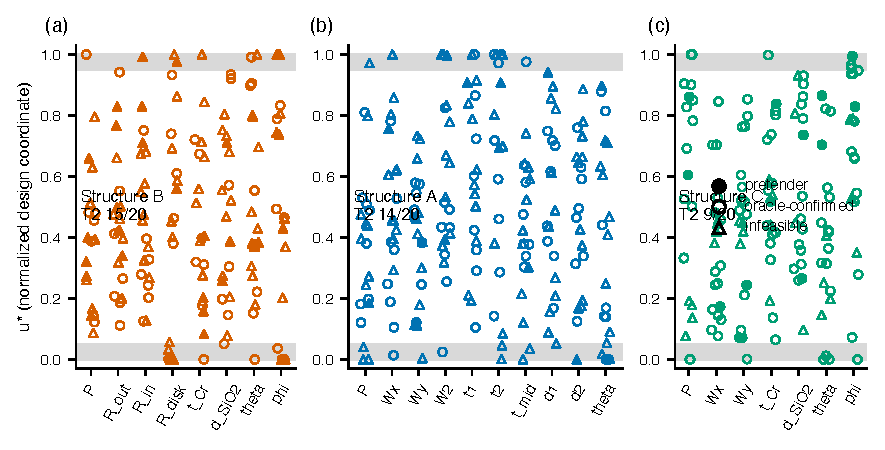
\includegraphics{figures/figS1_box_edge_geometry.pdf}
\caption{Per-parameter position of every committed geometry inside the design box (seed 42; one column per design parameter, y = the normalized coordinate u*). Grey bands mark the T2 box-edge region, within 0.05 of either bound. Filled markers are pretenders and open markers oracle-confirmed designs; triangles are geometries that violate a generator constraint. The in-band counts equal the T2 totals of Supplementary Table S1.}
\label{sfig:S1}
\end{figure}

\begin{figure}[htbp]
\centering
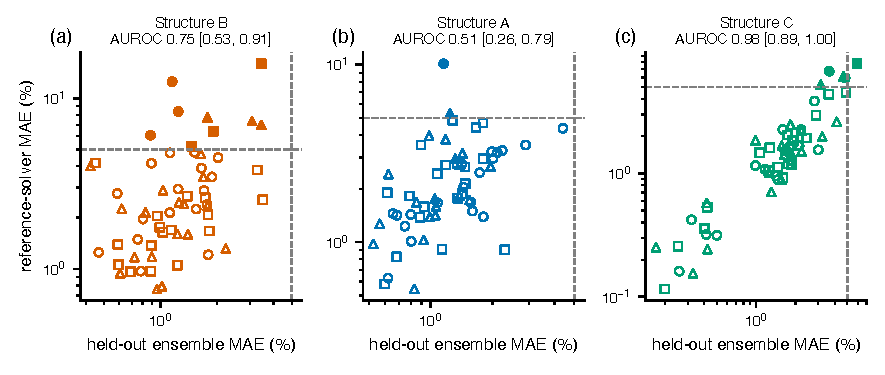
\includegraphics{figures/figS2_heldout_vs_rcwa.pdf}
\caption{Held-out ensemble error against reference-solver error for every valid committed geometry, per structure and training seed (log-log). The held-out ensemble error is the mean absolute error of the two surrogates that did \emph{not} commit the design, so it is available without any solver call. Dashed lines mark tau = 5 \%; filled markers are pretenders. Panel titles give the pooled AUROC for separating pretenders from oracle-confirmed designs, with its bootstrap 95 \% interval.}
\label{sfig:S2}
\end{figure}

\section*{S8. The as-submitted arm of Section 3.10}

The identical protocol run end to end on the release of \cite{choi20261} that the published pipeline superseded (upstream commit \texttt{920b1bd}; fixed Fourier order 5, complex128; datasets struct\_A\_vis\_500 (479 good, 380--780 nm), struct\_B\_500 (461, 400--1800 nm), struct\_C\_500 (400, 400--1800 nm); C trained on 300 samples with a {[}50, 400{]} nm normalization box and 13 physics features). Artifacts: \texttt{results\_v8/}. The tables below are the S1, S2 and S6 equivalents for that arm.

\begin{landscape}
\subsection*{S8.1. Per-run reliability accounting (as-submitted arm)}

\begingroup
\setlength{\tabcolsep}{2pt}\tiny
\captionof{table}{Per-run reliability accounting (as-submitted arm)}
\label{stab:8}
{\def\LTcaptype{none} % do not increment counter
\begin{longtable}[]{@{}lllllllllllllllll@{}}
\toprule\noalign{}
S & seed & n\_valid & surrogate-claimed {[}Wilson 95 \%{]} & oracle-confirmed {[}Wilson{]} & pretenders {[}Wilson{]} & \ensuremath{\Delta}-flagged {[}Wilson{]} & flag thr (\%) & modes & T1 & T2 & T3 & T4 & tail RSD & endpoint spread (u) & \ensuremath{\rho}(RCWA, Surr) {[}CI95{]} & p \\
\midrule\noalign{}
\endhead
\bottomrule\noalign{}
\endlastfoot
A & 42 & 20 & 20 {[}83.9, 100.0{]} & 11 {[}34.2, 74.2{]} & 9 {[}25.8, 65.8{]} & 0 {[}0.0, 16.1{]} & 9.69 & 20 & 19 & 15 & 0 & 0 & 0.0175 & 1.978 & +0.18 {[}-0.28, 0.58{]} & 0.435 \\
A & 123 & 20 & 20 {[}83.9, 100.0{]} & 11 {[}34.2, 74.2{]} & 9 {[}25.8, 65.8{]} & 1 {[}0.9, 23.6{]} & 9.68 & 18 & 19 & 16 & 3 & 0 & 0.0257 & 1.98 & +0.39 {[}-0.08, 0.72{]} & 0.086 \\
A & 777 & 20 & 20 {[}83.9, 100.0{]} & 11 {[}34.2, 74.2{]} & 9 {[}25.8, 65.8{]} & 1 {[}0.9, 23.6{]} & 9.46 & 19 & 20 & 16 & 2 & 0 & 0.0138 & 2.019 & +0.45 {[}-0.02, 0.75{]} & 0.048 \\
B & 42 & 20 & 20 {[}83.9, 100.0{]} & 11 {[}34.2, 74.2{]} & 9 {[}25.8, 65.8{]} & 6 {[}14.5, 51.9{]} & 6.37 & 17 & 16 & 14 & 5 & 0 & 0.0127 & 1.64 & -0.03 {[}-0.47, 0.42{]} & 0.890 \\
B & 123 & 20 & 20 {[}83.9, 100.0{]} & 9 {[}25.8, 65.8{]} & 11 {[}34.2, 74.2{]} & 8 {[}21.9, 61.3{]} & 6.52 & 18 & 20 & 16 & 4 & 0 & 0.0084 & 1.643 & -0.11 {[}-0.53, 0.35{]} & 0.654 \\
B & 777 & 20 & 20 {[}83.9, 100.0{]} & 10 {[}29.9, 70.1{]} & 10 {[}29.9, 70.1{]} & 6 {[}14.5, 51.9{]} & 6.56 & 15 & 18 & 14 & 7 & 0 & 0.0239 & 1.69 & +0.20 {[}-0.27, 0.60{]} & 0.391 \\
C & 42 & 20 & 20 {[}83.9, 100.0{]} & 7 {[}18.1, 56.7{]} & 13 {[}43.3, 81.9{]} & 3 {[}5.2, 36.0{]} & 7.73 & 15 & 11 & 11 & 7 & 0 & 0.0171 & 1.62 & -0.04 {[}-0.47, 0.41{]} & 0.880 \\
C & 123 & 20 & 20 {[}83.9, 100.0{]} & 8 {[}21.9, 61.3{]} & 12 {[}38.7, 78.1{]} & 2 {[}2.8, 30.1{]} & 7.66 & 13 & 11 & 12 & 10 & 0 & 0.0145 & 1.624 & +0.53 {[}0.08, 0.80{]} & 0.016 \\
C & 777 & 19 & 19 {[}83.2, 100.0{]} & 6 {[}15.4, 54.0{]} & 13 {[}46.0, 84.6{]} & 2 {[}2.9, 31.4{]} & 8.0 & 15 & 11 & 12 & 7 & 0 & 0.0021 & 1.676 & +0.28 {[}-0.21, 0.65{]} & 0.254 \\
\textbf{all} & & 179 & & & \textbf{95/179} (A 27/60, B 30/60, C 38/59) & & & & & & & & & & & \\
\end{longtable}
}
\endgroup
\end{landscape}

\begin{landscape}
\subsection*{S8.2. Commitment-rule comparison (seed 42; as-submitted arm)}

\begingroup
\setlength{\tabcolsep}{2pt}\tiny
\captionof{table}{Commitment-rule comparison (seed 42; as-submitted arm)}
\label{stab:9}
{\def\LTcaptype{none} % do not increment counter
\begin{longtable}[]{@{}lllllllll@{}}
\toprule\noalign{}
S & rule & surrogate-claimed & oracle-confirmed & pretenders (of n) & pretenders / claimed {[}Wilson{]} & mean oracle MAE (\%) & Fisher p vs best-of-8 (design-level) & Fisher p (conditional on claimed) \\
\midrule\noalign{}
\endhead
\bottomrule\noalign{}
\endlastfoot
A & gradient best-of-8 & 20 & 11 & 9/20 & 9/20 {[}25.8, 65.8{]} & 4.85 & --- & --- \\
A & random search (budget-matched) & 19 & 9 & 10/20 & 10/19 {[}31.7, 72.7{]} & 5.45 & 1.000 & 0.752 \\
A & single start (mid-box) & 20 & 12 & 8/20 & 8/20 {[}21.9, 61.3{]} & 5.49 & 1.000 & 1.000 \\
B & gradient best-of-8 & 20 & 11 & 9/20 & 9/20 {[}25.8, 65.8{]} & 6.65 & --- & --- \\
B & random search (budget-matched) & 19 & 5 & 14/20 & 14/19 {[}51.2, 88.2{]} & 10.79 & 0.200 & 0.105 \\
B & single start (mid-box) & 20 & 11 & 9/20 & 9/20 {[}25.8, 65.8{]} & 5.96 & 1.000 & 1.000 \\
C & gradient best-of-8 & 20 & 7 & 13/20 & 13/20 {[}43.3, 81.9{]} & 6.85 & --- & --- \\
C & random search (budget-matched) & 16 & 0 & 16/20 & 16/16 {[}80.6, 100.0{]} & 9.17 & 0.480 & 0.011 \\
C & single start (mid-box) & 17 & 8 & 9/20 & 9/17 {[}31.0, 73.8{]} & 7.18 & 0.341 & 0.516 \\
\end{longtable}
}
\endgroup
\end{landscape}

\subsection*{S8.3. Per-design table (as-submitted arm)}

Source: \texttt{results\_v8/} (reliability, recoverability JSONs; rcwa npz). \ensuremath{\tau} = 5 \%. status: pretender = Surr \ensuremath{\leq} \ensuremath{\tau} \& RCWA \textgreater{} \ensuremath{\tau}; confirmed = both \ensuremath{\leq} \ensuremath{\tau}; honest-failure = Surr \textgreater{} \ensuremath{\tau}; degenerate = solver failure.

\begingroup
\setlength{\tabcolsep}{2pt}\tiny
\captionof{table}{Per-design table (as-submitted arm)}
\label{stab:10}
{\def\LTcaptype{none} % do not increment counter
\begin{longtable}[]{@{}lllllllllllllllll@{}}
\toprule\noalign{}
S & seed & \# & idx & Surr MAE \% & RCWA MAE \% & \ensuremath{\Delta} pp & status & T1 & T2 & T3 & T4 & Surr@truth \% & \ensuremath{\|}u*\ensuremath{-}u\_true\ensuremath{\|} & support viol. & peak shift nm & peak \ensuremath{\Delta}A \\
\midrule\noalign{}
\endhead
\bottomrule\noalign{}
\endlastfoot
A & 42 & 1 & 190 & 0.07 & 1.74 & +1.67 & confirmed & 1 & 1 & 0 & 0 & 2.73 & 1.15 & 0 & +0 & -0.01 \\
A & 42 & 2 & 381 & 0.56 & 2.84 & +2.28 & confirmed & 1 & 1 & 0 & 0 & 4.01 & 1.15 & 0 & -12 & +0.02 \\
A & 42 & 3 & 451 & 1.22 & 2.74 & +1.52 & confirmed & 0 & 1 & 0 & 0 & 5.13 & 1.01 & 0 & +12 & -0.01 \\
A & 42 & 4 & 456 & 0.05 & 2.54 & +2.49 & confirmed & 1 & 1 & 0 & 0 & 0.66 & 1.47 & 1 & +0 & +0.00 \\
A & 42 & 5 & 482 & 0.17 & 7.56 & +7.38 & pretender & 1 & 1 & 0 & 0 & 2.72 & 1.12 & 1 & +109 & +0.11 \\
A & 42 & 6 & 24 & 0.47 & 7.42 & +6.95 & pretender & 1 & 1 & 0 & 0 & 5.83 & 0.75 & 0 & -48 & +0.18 \\
A & 42 & 7 & 16 & 0.47 & 3.26 & +2.79 & confirmed & 1 & 1 & 0 & 0 & 9.79 & 1.43 & 1 & +4 & +0.10 \\
A & 42 & 8 & 289 & 0.27 & 2.90 & +2.64 & confirmed & 1 & 0 & 0 & 0 & 2.65 & 1.24 & 0 & +4 & +0.02 \\
A & 42 & 9 & 327 & 0.21 & 5.83 & +5.62 & pretender & 1 & 1 & 0 & 0 & 6.77 & 1.41 & 1 & -28 & +0.01 \\
A & 42 & 10 & 101 & 0.63 & 6.76 & +6.13 & pretender & 1 & 1 & 0 & 0 & 4.37 & 1.66 & 0 & +323 & +0.03 \\
A & 42 & 11 & 249 & 1.24 & 4.44 & +3.19 & confirmed & 1 & 1 & 0 & 0 & 7.54 & 1.11 & 0 & -24 & -0.01 \\
A & 42 & 12 & 25 & 0.45 & 3.06 & +2.61 & confirmed & 1 & 0 & 0 & 0 & 5.14 & 0.74 & 0 & +12 & +0.08 \\
A & 42 & 13 & 37 & 1.00 & 4.26 & +3.26 & confirmed & 1 & 0 & 0 & 0 & 4.21 & 1.36 & 1 & -16 & -0.02 \\
A & 42 & 14 & 481 & 0.21 & 6.50 & +6.29 & pretender & 1 & 1 & 0 & 0 & 6.22 & 1.18 & 1 & +61 & +0.12 \\
A & 42 & 15 & 246 & 1.43 & 6.48 & +5.05 & pretender & 1 & 1 & 0 & 0 & 5.36 & 0.78 & 0 & +20 & -0.02 \\
A & 42 & 16 & 43 & 0.37 & 6.73 & +6.36 & pretender & 1 & 1 & 0 & 0 & 3.20 & 0.99 & 1 & +28 & +0.12 \\
A & 42 & 17 & 333 & 0.60 & 4.22 & +3.63 & confirmed & 1 & 0 & 0 & 0 & 5.10 & 1.08 & 0 & +20 & +0.06 \\
A & 42 & 18 & 312 & 1.46 & 7.36 & +5.90 & pretender & 1 & 0 & 0 & 0 & 6.63 & 0.74 & 1 & -16 & +0.15 \\
A & 42 & 19 & 6 & 0.20 & 5.92 & +5.72 & pretender & 1 & 1 & 0 & 0 & 4.44 & 0.92 & 1 & -4 & +0.12 \\
A & 42 & 20 & 413 & 0.08 & 4.36 & +4.28 & confirmed & 1 & 1 & 0 & 0 & 0.96 & 1.39 & 1 & +0 & +0.04 \\
A & 123 & 1 & 190 & 0.04 & 2.14 & +2.10 & confirmed & 1 & 1 & 0 & 0 & 3.85 & 0.99 & 0 & +0 & -0.01 \\
A & 123 & 2 & 381 & 0.73 & 4.04 & +3.31 & confirmed & 1 & 1 & 0 & 0 & 4.83 & 1.45 & 0 & +0 & +0.05 \\
A & 123 & 3 & 451 & 1.04 & 4.60 & +3.56 & confirmed & 1 & 1 & 0 & 0 & 5.79 & 0.73 & 1 & +12 & +0.02 \\
A & 123 & 4 & 456 & 0.06 & 10.08 & +10.02 & pretender & 1 & 1 & 0 & 0 & 0.61 & 1.33 & 1 & +77 & +0.31 \\
A & 123 & 5 & 482 & 0.10 & 4.37 & +4.27 & confirmed & 1 & 1 & 0 & 0 & 3.12 & 1.45 & 1 & +0 & -0.03 \\
A & 123 & 6 & 24 & 0.31 & 8.76 & +8.45 & pretender & 1 & 1 & 0 & 0 & 6.51 & 1.10 & 0 & -81 & +0.14 \\
A & 123 & 7 & 16 & 0.50 & 7.13 & +6.63 & pretender & 1 & 1 & 0 & 0 & 9.40 & 1.65 & 0 & -97 & -0.01 \\
A & 123 & 8 & 289 & 0.32 & 3.97 & +3.65 & confirmed & 1 & 1 & 1 & 0 & 3.49 & 1.07 & 0 & -8 & +0.03 \\
A & 123 & 9 & 327 & 0.52 & 5.81 & +5.29 & pretender & 1 & 1 & 0 & 0 & 7.09 & 1.39 & 0 & -28 & -0.08 \\
A & 123 & 10 & 101 & 0.53 & 3.98 & +3.45 & confirmed & 1 & 1 & 0 & 0 & 2.21 & 1.61 & 1 & +8 & +0.11 \\
A & 123 & 11 & 249 & 0.57 & 4.65 & +4.08 & confirmed & 1 & 0 & 0 & 0 & 5.47 & 0.56 & 0 & -8 & -0.01 \\
A & 123 & 12 & 25 & 0.39 & 9.12 & +8.73 & pretender & 1 & 0 & 1 & 0 & 4.30 & 1.17 & 0 & -20 & +0.04 \\
A & 123 & 13 & 37 & 0.75 & 7.94 & +7.19 & pretender & 1 & 0 & 0 & 0 & 4.96 & 1.38 & 1 & +12 & +0.06 \\
A & 123 & 14 & 481 & 0.25 & 3.50 & +3.25 & confirmed & 1 & 1 & 0 & 0 & 6.43 & 0.95 & 1 & -12 & +0.03 \\
A & 123 & 15 & 246 & 2.63 & 6.81 & +4.18 & pretender & 0 & 1 & 0 & 0 & 4.44 & 0.50 & 0 & +32 & +0.05 \\
A & 123 & 16 & 43 & 0.24 & 2.82 & +2.59 & confirmed & 1 & 1 & 0 & 0 & 3.34 & 0.90 & 0 & -8 & +0.03 \\
A & 123 & 17 & 333 & 0.65 & 8.08 & +7.42 & pretender & 1 & 0 & 1 & 0 & 3.18 & 0.96 & 0 & +36 & -0.02 \\
A & 123 & 18 & 312 & 2.33 & 9.62 & +7.29 & pretender & 1 & 1 & 0 & 0 & 8.95 & 0.74 & 1 & -24 & +0.13 \\
A & 123 & 19 & 6 & 0.11 & 3.17 & +3.06 & confirmed & 1 & 1 & 0 & 0 & 10.10 & 0.99 & 0 & -32 & -0.00 \\
A & 123 & 20 & 413 & 0.06 & 4.26 & +4.20 & confirmed & 1 & 1 & 0 & 0 & 0.54 & 1.52 & 0 & +0 & -0.05 \\
A & 777 & 1 & 190 & 0.10 & 1.65 & +1.55 & confirmed & 1 & 0 & 1 & 0 & 1.36 & 1.49 & 1 & +0 & -0.01 \\
A & 777 & 2 & 381 & 0.64 & 4.80 & +4.16 & confirmed & 1 & 1 & 0 & 0 & 2.92 & 1.08 & 1 & +0 & +0.02 \\
A & 777 & 3 & 451 & 0.79 & 4.04 & +3.25 & confirmed & 1 & 0 & 0 & 0 & 5.63 & 1.00 & 0 & +12 & -0.00 \\
A & 777 & 4 & 456 & 0.05 & 3.82 & +3.77 & confirmed & 1 & 1 & 0 & 0 & 1.85 & 0.83 & 0 & +0 & -0.03 \\
A & 777 & 5 & 482 & 0.12 & 4.63 & +4.51 & confirmed & 1 & 1 & 0 & 0 & 0.70 & 1.61 & 0 & +0 & -0.03 \\
A & 777 & 6 & 24 & 0.39 & 3.96 & +3.57 & confirmed & 1 & 1 & 0 & 0 & 4.57 & 0.93 & 0 & -28 & +0.08 \\
A & 777 & 7 & 16 & 0.48 & 4.73 & +4.25 & confirmed & 1 & 0 & 0 & 0 & 9.69 & 1.17 & 0 & +4 & -0.09 \\
A & 777 & 8 & 289 & 0.33 & 6.11 & +5.77 & pretender & 1 & 1 & 0 & 0 & 2.81 & 1.04 & 0 & -20 & -0.02 \\
A & 777 & 9 & 327 & 0.47 & 6.63 & +6.16 & pretender & 1 & 1 & 0 & 0 & 6.93 & 1.26 & 1 & -24 & +0.01 \\
A & 777 & 10 & 101 & 0.64 & 11.17 & +10.52 & pretender & 1 & 1 & 0 & 0 & 3.73 & 1.11 & 0 & +186 & +0.11 \\
A & 777 & 11 & 249 & 0.68 & 7.44 & +6.76 & pretender & 1 & 1 & 0 & 0 & 6.71 & 0.71 & 0 & +44 & -0.05 \\
A & 777 & 12 & 25 & 0.25 & 6.63 & +6.37 & pretender & 1 & 1 & 0 & 0 & 6.24 & 1.18 & 0 & +40 & +0.06 \\
A & 777 & 13 & 37 & 0.75 & 2.58 & +1.83 & confirmed & 1 & 1 & 0 & 0 & 4.63 & 1.41 & 0 & -4 & +0.02 \\
A & 777 & 14 & 481 & 0.14 & 1.97 & +1.83 & confirmed & 1 & 0 & 0 & 0 & 6.49 & 0.40 & 0 & -12 & -0.04 \\
A & 777 & 15 & 246 & 0.69 & 9.73 & +9.04 & pretender & 1 & 1 & 0 & 0 & 4.97 & 1.07 & 0 & -283 & -0.02 \\
A & 777 & 16 & 43 & 0.16 & 4.39 & +4.23 & confirmed & 1 & 1 & 0 & 0 & 3.93 & 1.14 & 0 & +44 & +0.02 \\
A & 777 & 17 & 333 & 0.51 & 7.36 & +6.85 & pretender & 1 & 1 & 0 & 0 & 2.69 & 1.33 & 0 & +48 & +0.07 \\
A & 777 & 18 & 312 & 1.48 & 5.32 & +3.84 & pretender & 1 & 1 & 0 & 0 & 7.92 & 1.18 & 0 & -81 & -0.10 \\
A & 777 & 19 & 6 & 0.71 & 5.21 & +4.50 & pretender & 1 & 1 & 0 & 0 & 9.07 & 1.21 & 0 & +0 & -0.00 \\
A & 777 & 20 & 413 & 0.07 & 3.36 & +3.29 & confirmed & 1 & 1 & 1 & 0 & 0.76 & 1.04 & 0 & +0 & -0.03 \\
B & 42 & 1 & 358 & 0.45 & 1.84 & +1.38 & confirmed & 1 & 0 & 1 & 0 & 3.65 & 0.63 & 0 & +28 & -0.03 \\
B & 42 & 2 & 43 & 1.14 & 2.60 & +1.46 & confirmed & 0 & 1 & 0 & 0 & 3.06 & 0.37 & 0 & +14 & +0.02 \\
B & 42 & 3 & 24 & 0.76 & 3.80 & +3.05 & confirmed & 1 & 0 & 1 & 0 & 3.14 & 0.59 & 0 & +28 & -0.02 \\
B & 42 & 4 & 428 & 0.43 & 3.76 & +3.33 & confirmed & 1 & 1 & 0 & 0 & 2.87 & 0.78 & 0 & +71 & +0.04 \\
B & 42 & 5 & 487 & 1.07 & 1.96 & +0.88 & confirmed & 0 & 0 & 0 & 0 & 1.66 & 0.21 & 0 & +0 & +0.00 \\
B & 42 & 6 & 396 & 1.10 & 1.62 & +0.52 & confirmed & 0 & 1 & 0 & 0 & 2.93 & 0.26 & 0 & +14 & -0.03 \\
B & 42 & 7 & 302 & 0.61 & 31.64 & +31.03 & pretender & 1 & 1 & 0 & 0 & 6.10 & 1.20 & 1 & +933 & +0.29 \\
B & 42 & 8 & 468 & 0.63 & 5.86 & +5.23 & pretender & 1 & 1 & 0 & 0 & 3.90 & 0.66 & 0 & -339 & -0.03 \\
B & 42 & 9 & 310 & 0.70 & 2.78 & +2.08 & confirmed & 1 & 1 & 0 & 0 & 3.09 & 0.74 & 0 & +57 & -0.01 \\
B & 42 & 10 & 38 & 1.88 & 6.82 & +4.95 & pretender & 1 & 1 & 0 & 0 & 7.98 & 0.50 & 0 & +14 & +0.10 \\
B & 42 & 11 & 16 & 1.03 & 2.51 & +1.48 & confirmed & 0 & 1 & 0 & 0 & 2.71 & 0.39 & 0 & +28 & -0.01 \\
B & 42 & 12 & 168 & 0.35 & 7.58 & +7.23 & pretender & 1 & 1 & 1 & 0 & 2.17 & 0.87 & 0 & -57 & -0.07 \\
B & 42 & 13 & 339 & 0.30 & 2.56 & +2.25 & confirmed & 1 & 0 & 0 & 0 & 3.39 & 0.60 & 0 & +42 & -0.04 \\
B & 42 & 14 & 146 & 0.30 & 7.54 & +7.24 & pretender & 1 & 0 & 0 & 0 & 1.89 & 0.46 & 0 & +28 & -0.09 \\
B & 42 & 15 & 118 & 0.31 & 1.49 & +1.18 & confirmed & 1 & 0 & 1 & 0 & 4.22 & 0.73 & 0 & -28 & +0.04 \\
B & 42 & 16 & 481 & 1.22 & 7.25 & +6.03 & pretender & 1 & 1 & 0 & 0 & 4.92 & 0.64 & 0 & +71 & +0.02 \\
B & 42 & 17 & 172 & 0.37 & 10.74 & +10.37 & pretender & 1 & 1 & 0 & 0 & 4.17 & 0.48 & 0 & +438 & +0.21 \\
B & 42 & 18 & 311 & 0.67 & 13.40 & +12.72 & pretender & 1 & 1 & 1 & 0 & 2.77 & 0.34 & 0 & -820 & -0.06 \\
B & 42 & 19 & 51 & 0.49 & 3.53 & +3.04 & confirmed & 1 & 1 & 0 & 0 & 1.81 & 0.71 & 0 & +0 & -0.08 \\
B & 42 & 20 & 255 & 1.07 & 13.68 & +12.61 & pretender & 1 & 1 & 0 & 0 & 1.59 & 1.68 & 0 & +0 & +0.18 \\
B & 123 & 1 & 358 & 0.65 & 7.31 & +6.66 & pretender & 1 & 0 & 1 & 0 & 4.04 & 0.85 & 0 & -71 & +0.00 \\
B & 123 & 2 & 43 & 0.97 & 4.53 & +3.56 & confirmed & 1 & 1 & 0 & 0 & 3.53 & 0.45 & 0 & +28 & +0.02 \\
B & 123 & 3 & 24 & 0.47 & 3.77 & +3.31 & confirmed & 1 & 0 & 1 & 0 & 2.45 & 0.45 & 0 & +42 & +0.01 \\
B & 123 & 4 & 428 & 0.56 & 3.50 & +2.94 & confirmed & 1 & 1 & 0 & 0 & 3.27 & 0.51 & 0 & -14 & +0.04 \\
B & 123 & 5 & 487 & 1.15 & 3.89 & +2.74 & confirmed & 1 & 1 & 0 & 0 & 1.36 & 0.35 & 0 & -99 & -0.00 \\
B & 123 & 6 & 396 & 0.90 & 2.91 & +2.01 & confirmed & 1 & 0 & 1 & 0 & 2.58 & 0.52 & 0 & +99 & -0.03 \\
B & 123 & 7 & 302 & 0.56 & 16.43 & +15.87 & pretender & 1 & 1 & 0 & 0 & 5.42 & 1.21 & 1 & +749 & +0.11 \\
B & 123 & 8 & 468 & 0.39 & 10.68 & +10.29 & pretender & 1 & 1 & 0 & 0 & 6.64 & 1.14 & 0 & +424 & +0.21 \\
B & 123 & 9 & 310 & 0.61 & 3.07 & +2.46 & confirmed & 1 & 1 & 0 & 0 & 2.19 & 0.88 & 0 & -14 & -0.02 \\
B & 123 & 10 & 38 & 1.36 & 5.35 & +3.99 & pretender & 1 & 1 & 0 & 0 & 10.67 & 0.83 & 0 & -57 & +0.05 \\
B & 123 & 11 & 16 & 0.90 & 6.87 & +5.97 & pretender & 1 & 1 & 0 & 0 & 2.85 & 0.43 & 0 & +0 & -0.04 \\
B & 123 & 12 & 168 & 0.59 & 25.79 & +25.20 & pretender & 1 & 1 & 0 & 0 & 2.59 & 1.24 & 0 & -156 & -0.19 \\
B & 123 & 13 & 339 & 0.32 & 3.75 & +3.43 & confirmed & 1 & 0 & 0 & 0 & 1.99 & 0.64 & 0 & +0 & -0.06 \\
B & 123 & 14 & 146 & 0.30 & 9.42 & +9.12 & pretender & 1 & 1 & 0 & 0 & 1.05 & 0.90 & 0 & +57 & -0.12 \\
B & 123 & 15 & 118 & 0.34 & 26.96 & +26.62 & pretender & 1 & 1 & 1 & 0 & 3.04 & 1.06 & 0 & -636 & -0.30 \\
B & 123 & 16 & 481 & 1.12 & 4.50 & +3.38 & confirmed & 1 & 1 & 0 & 0 & 5.59 & 0.45 & 0 & +57 & +0.08 \\
B & 123 & 17 & 172 & 0.42 & 10.17 & +9.74 & pretender & 1 & 1 & 0 & 0 & 2.45 & 0.41 & 0 & +537 & +0.13 \\
B & 123 & 18 & 311 & 1.02 & 5.51 & +4.50 & pretender & 1 & 1 & 0 & 0 & 5.03 & 1.26 & 0 & -552 & +0.13 \\
B & 123 & 19 & 51 & 0.53 & 2.01 & +1.47 & confirmed & 1 & 1 & 0 & 0 & 2.68 & 0.72 & 0 & -14 & -0.01 \\
B & 123 & 20 & 255 & 1.47 & 17.50 & +16.03 & pretender & 1 & 1 & 0 & 0 & 2.70 & 1.37 & 0 & -57 & +0.14 \\
B & 777 & 1 & 358 & 0.64 & 1.69 & +1.05 & confirmed & 0 & 0 & 1 & 0 & 3.99 & 0.75 & 0 & -14 & -0.02 \\
B & 777 & 2 & 43 & 1.00 & 2.08 & +1.07 & confirmed & 0 & 1 & 1 & 0 & 4.39 & 0.41 & 0 & +14 & -0.01 \\
B & 777 & 3 & 24 & 0.45 & 2.56 & +2.11 & confirmed & 1 & 0 & 1 & 0 & 3.07 & 0.73 & 0 & +0 & +0.01 \\
B & 777 & 4 & 428 & 0.42 & 4.07 & +3.66 & confirmed & 1 & 1 & 0 & 0 & 2.90 & 0.64 & 0 & +0 & +0.03 \\
B & 777 & 5 & 487 & 1.26 & 4.44 & +3.18 & confirmed & 1 & 0 & 1 & 0 & 2.08 & 0.27 & 0 & -113 & -0.00 \\
B & 777 & 6 & 396 & 1.00 & 3.16 & +2.16 & confirmed & 1 & 0 & 1 & 0 & 2.57 & 0.21 & 0 & +0 & +0.00 \\
B & 777 & 7 & 302 & 1.16 & 12.76 & +11.60 & pretender & 1 & 1 & 0 & 0 & 4.89 & 1.31 & 1 & +0 & +0.10 \\
B & 777 & 8 & 468 & 0.79 & 12.28 & +11.48 & pretender & 1 & 0 & 1 & 0 & 6.12 & 1.03 & 0 & -665 & -0.10 \\
B & 777 & 9 & 310 & 0.71 & 2.16 & +1.45 & confirmed & 1 & 1 & 0 & 0 & 2.22 & 0.79 & 0 & -14 & -0.02 \\
B & 777 & 10 & 38 & 1.61 & 7.03 & +5.42 & pretender & 1 & 1 & 0 & 0 & 9.30 & 0.78 & 1 & +28 & -0.02 \\
B & 777 & 11 & 16 & 0.86 & 6.27 & +5.42 & pretender & 1 & 1 & 1 & 0 & 3.27 & 0.45 & 0 & +0 & -0.07 \\
B & 777 & 12 & 168 & 0.24 & 5.52 & +5.28 & pretender & 1 & 0 & 0 & 0 & 2.63 & 0.79 & 0 & +1089 & +0.00 \\
B & 777 & 13 & 339 & 0.30 & 4.49 & +4.19 & confirmed & 1 & 1 & 0 & 0 & 1.68 & 0.53 & 0 & -14 & -0.06 \\
B & 777 & 14 & 146 & 0.25 & 5.16 & +4.91 & pretender & 1 & 1 & 0 & 0 & 1.63 & 0.50 & 0 & +99 & -0.04 \\
B & 777 & 15 & 118 & 0.51 & 33.58 & +33.07 & pretender & 1 & 1 & 0 & 0 & 4.00 & 1.22 & 0 & -42 & -0.36 \\
B & 777 & 16 & 481 & 1.13 & 4.96 & +3.82 & confirmed & 1 & 1 & 0 & 0 & 5.83 & 0.59 & 0 & +71 & +0.09 \\
B & 777 & 17 & 172 & 0.34 & 4.64 & +4.29 & confirmed & 1 & 1 & 0 & 0 & 3.21 & 0.91 & 0 & -42 & +0.06 \\
B & 777 & 18 & 311 & 1.11 & 9.27 & +8.16 & pretender & 1 & 1 & 0 & 0 & 5.04 & 1.43 & 0 & -834 & -0.06 \\
B & 777 & 19 & 51 & 0.80 & 21.24 & +20.44 & pretender & 1 & 1 & 0 & 0 & 2.43 & 0.80 & 1 & +14 & -0.32 \\
B & 777 & 20 & 255 & 1.02 & 13.14 & +12.13 & pretender & 1 & 1 & 0 & 0 & 1.82 & 1.41 & 0 & +1343 & +0.22 \\
C & 42 & 1 & 363 & 2.57 & 9.15 & +6.58 & pretender & 1 & 1 & 0 & 0 & 5.92 & 0.84 & 1 & +14/-255 & +0.54/+0.05 \\
C & 42 & 2 & 221 & 0.50 & 3.60 & +3.10 & confirmed & 1 & 0 & 1 & 0 & 2.59 & 0.76 & 0 & +127/+42 & +0.07/+0.02 \\
C & 42 & 3 & 399 & 2.16 & 3.79 & +1.63 & confirmed & 0 & 0 & 1 & 0 & 6.11 & 0.63 & 0 & -99/+0 & +0.08/+0.01 \\
C & 42 & 4 & 382 & 1.75 & 3.42 & +1.67 & confirmed & 0 & 0 & 0 & 0 & 2.61 & 0.18 & 0 & +14/+42 & -0.02/+0.00 \\
C & 42 & 5 & 121 & 1.09 & 3.37 & +2.28 & confirmed & 1 & 0 & 1 & 0 & 3.69 & 0.25 & 0 & +0/+156 & +0.04/+0.06 \\
C & 42 & 6 & 178 & 1.75 & 3.80 & +2.05 & confirmed & 0 & 0 & 0 & 0 & 2.63 & 0.46 & 0 & +0/+0 & +0.04/-0.00 \\
C & 42 & 7 & 203 & 3.88 & 5.59 & +1.71 & pretender & 0 & 0 & 1 & 0 & 9.29 & 0.42 & 0 & +382/+0 & +0.08/-0.01 \\
C & 42 & 8 & 341 & 0.42 & 5.72 & +5.30 & pretender & 1 & 0 & 1 & 0 & 1.10 & 0.11 & 0 & +113/-354 & +0.04/-0.11 \\
C & 42 & 9 & 139 & 1.36 & 6.87 & +5.51 & pretender & 1 & 1 & 0 & 0 & 2.41 & 0.28 & 1 & -113/+0 & +0.15/-0.02 \\
C & 42 & 10 & 244 & 3.29 & 6.49 & +3.20 & pretender & 0 & 1 & 0 & 0 & 5.70 & 0.69 & 0 & +127/+28 & +0.00/-0.10 \\
C & 42 & 11 & 176 & 3.88 & 11.06 & +7.18 & pretender & 0 & 1 & 0 & 0 & 2.56 & 0.94 & 0 & +42/+156 & +0.07/-0.19 \\
C & 42 & 12 & 271 & 0.83 & 5.67 & +4.84 & pretender & 1 & 0 & 1 & 0 & 3.32 & 0.50 & 0 & +1174/+0 & +0.11/+0.02 \\
C & 42 & 13 & 245 & 0.40 & 10.79 & +10.39 & pretender & 1 & 1 & 0 & 0 & 1.29 & 0.28 & 1 & +962/-410 & +0.34/-0.04 \\
C & 42 & 14 & 6 & 2.79 & 3.82 & +1.03 & confirmed & 0 & 1 & 0 & 0 & 3.93 & 0.18 & 0 & +226/-14 & -0.01/+0.01 \\
C & 42 & 15 & 208 & 0.87 & 14.54 & +13.67 & pretender & 1 & 1 & 0 & 0 & 2.14 & 0.33 & 0 & +848/-283 & +0.29/-0.12 \\
C & 42 & 16 & 129 & 2.01 & 3.99 & +1.98 & confirmed & 0 & 1 & 0 & 0 & 8.38 & 1.24 & 0 & -14/-127 & -0.02/-0.08 \\
C & 42 & 17 & 463 & 3.62 & 5.70 & +2.08 & pretender & 0 & 1 & 0 & 0 & 2.32 & 1.45 & 1 & +28/+156 & +0.00/-0.04 \\
C & 42 & 18 & 137 & 2.76 & 9.78 & +7.02 & pretender & 1 & 1 & 0 & 0 & 6.03 & 0.96 & 0 & -71/-28 & -0.07/-0.01 \\
C & 42 & 19 & 45 & 2.13 & 7.92 & +5.78 & pretender & 1 & 1 & 0 & 0 & 4.97 & 0.69 & 0 & +14/-42 & +0.03/+0.01 \\
C & 42 & 20 & 403 & 0.43 & 11.93 & +11.50 & pretender & 1 & 0 & 1 & 0 & 0.54 & 0.48 & 0 & +1400/+0 & +0.37/+0.00 \\
C & 123 & 1 & 363 & 2.40 & 9.22 & +6.82 & pretender & 1 & 1 & 1 & 0 & 4.50 & 0.73 & 1 & -14/-71 & +0.51/+0.09 \\
C & 123 & 2 & 221 & 0.47 & 3.50 & +3.02 & confirmed & 1 & 0 & 1 & 0 & 1.35 & 0.24 & 0 & -14/+85 & -0.02/+0.07 \\
C & 123 & 3 & 399 & 1.83 & 2.36 & +0.53 & confirmed & 0 & 0 & 1 & 0 & 4.87 & 0.43 & 0 & -57/+0 & +0.04/+0.05 \\
C & 123 & 4 & 382 & 1.70 & 3.66 & +1.96 & confirmed & 0 & 0 & 0 & 0 & 2.77 & 0.21 & 0 & -14/+57 & -0.02/+0.00 \\
C & 123 & 5 & 121 & 1.04 & 6.06 & +5.01 & pretender & 1 & 1 & 0 & 0 & 3.42 & 0.48 & 0 & +0/-608 & -0.03/-0.00 \\
C & 123 & 6 & 178 & 1.80 & 7.56 & +5.76 & pretender & 1 & 0 & 0 & 0 & 2.10 & 0.43 & 0 & +0/+14 & +0.07/-0.08 \\
C & 123 & 7 & 203 & 3.92 & 5.52 & +1.61 & pretender & 0 & 0 & 1 & 0 & 9.41 & 0.37 & 0 & +382/+0 & +0.14/-0.01 \\
C & 123 & 8 & 341 & 0.42 & 6.85 & +6.43 & pretender & 1 & 0 & 1 & 0 & 0.94 & 0.19 & 0 & -156/-99 & -0.08/-0.09 \\
C & 123 & 9 & 139 & 1.89 & 2.73 & +0.84 & confirmed & 0 & 1 & 0 & 0 & 2.41 & 0.79 & 0 & +42/+85 & -0.07/+0.04 \\
C & 123 & 10 & 244 & 4.06 & 8.89 & +4.84 & pretender & 0 & 1 & 0 & 0 & 6.51 & 1.10 & 0 & -834/-170 & -0.01/+0.05 \\
C & 123 & 11 & 176 & 3.13 & 8.02 & +4.89 & pretender & 0 & 1 & 1 & 0 & 2.44 & 1.22 & 0 & +368/-28 & -0.01/-0.24 \\
C & 123 & 12 & 271 & 0.73 & 4.54 & +3.81 & confirmed & 1 & 0 & 0 & 0 & 2.73 & 0.64 & 0 & +0/+1259 & +0.01/+0.03 \\
C & 123 & 13 & 245 & 0.37 & 5.56 & +5.19 & pretender & 1 & 0 & 1 & 0 & 2.20 & 1.09 & 1 & +424/-438 & +0.02/-0.06 \\
C & 123 & 14 & 6 & 3.32 & 3.67 & +0.36 & confirmed & 0 & 1 & 1 & 0 & 4.44 & 0.19 & 0 & +226/-28 & -0.00/+0.00 \\
C & 123 & 15 & 208 & 0.43 & 2.62 & +2.18 & confirmed & 1 & 1 & 1 & 0 & 2.31 & 0.39 & 0 & +42/-113 & +0.02/-0.03 \\
C & 123 & 16 & 129 & 2.72 & 7.82 & +5.10 & pretender & 0 & 1 & 0 & 0 & 7.89 & 1.25 & 0 & -71/+14 & -0.02/+0.16 \\
C & 123 & 17 & 463 & 4.20 & 14.46 & +10.26 & pretender & 1 & 1 & 0 & 0 & 3.62 & 1.52 & 1 & -339/+14 & +0.40/+0.26 \\
C & 123 & 18 & 137 & 3.60 & 6.80 & +3.20 & pretender & 0 & 1 & 0 & 0 & 5.62 & 0.86 & 0 & -28/-57 & -0.05/-0.01 \\
C & 123 & 19 & 45 & 2.49 & 11.26 & +8.77 & pretender & 1 & 1 & 0 & 0 & 5.38 & 0.74 & 0 & +71/-42 & +0.01/-0.01 \\
C & 123 & 20 & 403 & 0.42 & 2.38 & +1.96 & confirmed & 1 & 1 & 1 & 0 & 0.72 & 0.12 & 0 & +0/+0 & +0.02/+0.01 \\
C & 777 & 1 & 363 & 2.27 & 7.54 & +5.26 & pretender & 1 & 0 & 0 & 0 & 3.93 & 0.75 & 1 & -14/+0 & +0.46/+0.09 \\
C & 777 & 2 & 221 & 0.47 & 7.82 & +7.35 & pretender & 1 & 1 & 1 & 0 & 2.01 & 1.10 & 0 & +156/+170 & +0.10/+0.12 \\
C & 777 & 3 & 399 & 2.16 & 5.93 & +3.77 & pretender & 0 & 1 & 1 & 0 & 5.84 & 1.10 & 0 & -113/+0 & +0.00/-0.05 \\
C & 777 & 4 & 382 & 1.78 & 3.45 & +1.68 & confirmed & 0 & 0 & 0 & 0 & 3.09 & 0.19 & 0 & +42/+28 & +0.01/+0.00 \\
C & 777 & 5 & 121 & 1.20 & 4.52 & +3.32 & confirmed & 1 & 1 & 1 & 0 & 3.89 & 0.47 & 0 & +0/-622 & -0.03/-0.01 \\
C & 777 & 6 & 178 & 2.25 & 5.20 & +2.95 & pretender & 0 & 0 & 0 & 0 & 2.31 & 0.41 & 0 & +14/+0 & +0.02/+0.03 \\
C & 777 & 7 & 203 & 4.66 & 5.50 & +0.84 & pretender & 0 & 0 & 1 & 0 & 9.45 & 0.37 & 0 & +382/+0 & +0.10/-0.02 \\
C & 777 & 8 & 341 & 0.25 & 3.71 & +3.46 & confirmed & 1 & 0 & 1 & 0 & 0.81 & 0.05 & 0 & -156/+14 & -0.09/+0.01 \\
C & 777 & 9 & 139 & 1.53 & 5.08 & +3.55 & pretender & 1 & 1 & 0 & 0 & 2.86 & 0.62 & 0 & +14/+0 & -0.11/-0.05 \\
C & 777 & 10 & 244 & 4.07 & 5.81 & +1.73 & pretender & 0 & 0 & 0 & 0 & 6.92 & 0.72 & 0 & -566/+14 & -0.07/-0.06 \\
C & 777 & 11 & 176 & 2.69 & 5.12 & +2.42 & pretender & 0 & 1 & 0 & 0 & 1.95 & 0.91 & 0 & +42/+42 & +0.04/-0.28 \\
C & 777 & 12 & 271 & 0.84 & 3.70 & +2.86 & confirmed & 1 & 0 & 0 & 0 & 4.80 & 0.47 & 0 & +1061/+0 & +0.07/+0.01 \\
C & 777 & 13 & 245 & 0.48 & 8.85 & +8.37 & pretender & 1 & 1 & 0 & 0 & 1.73 & 0.76 & 1 & -71/-438 & +0.35/+0.05 \\
C & 777 & 14 & 6 & 2.35 & 3.84 & +1.49 & confirmed & 0 & 1 & 0 & 0 & 3.96 & 0.15 & 0 & +212/-28 & +0.01/+0.01 \\
C & 777 & 15 & 208 & 1.57 & 5.68 & +4.11 & pretender & 1 & 0 & 1 & 0 & 2.44 & 1.36 & 0 & +71/-297 & +0.17/+0.03 \\
C & 777 & 16 & 129 & 2.91 & --- & --- & degenerate & 0 & 1 & 0 & 0 & 8.84 & 1.16 & 0 & +nan/+nan & +nan/+nan \\
C & 777 & 17 & 463 & 3.47 & 5.08 & +1.61 & pretender & 0 & 1 & 1 & 0 & 2.10 & 1.42 & 0 & +42/+127 & -0.00/-0.03 \\
C & 777 & 18 & 137 & 3.13 & 10.87 & +7.75 & pretender & 1 & 1 & 0 & 0 & 5.61 & 1.36 & 1 & -71/-212 & +0.11/-0.04 \\
C & 777 & 19 & 45 & 1.90 & 11.37 & +9.46 & pretender & 1 & 1 & 0 & 0 & 4.63 & 0.76 & 0 & +57/-42 & +0.02/-0.01 \\
C & 777 & 20 & 403 & 0.43 & 2.60 & +2.16 & confirmed & 1 & 1 & 0 & 0 & 0.58 & 0.06 & 0 & +0/+0 & -0.01/+0.01 \\
\end{longtable}
}
\endgroup

Valid designs: 179; pretenders: 95.


\end{document}
